%%%%%%%%%%%%%%%%%%%%%%%%%%%%%%%%%%%%%%%%%%%%%%%%%%%%%%%%%%%%
%%% LIVECOMS ARTICLE TEMPLATE FOR BEST PRACTICES GUIDE
%%% ADAPTED FROM ELIFE ARTICLE TEMPLATE (8/10/2017)
%%%%%%%%%%%%%%%%%%%%%%%%%%%%%%%%%%%%%%%%%%%%%%%%%%%%%%%%%%%%
%%% PREAMBLE
\documentclass[9pt,tutorial]{livecoms}
% Use the 'onehalfspacing' option for 1.5 line spacing
% Use the 'doublespacing' option for 2.0 line spacing
% Use the 'lineno' option for adding line numbers.
% Use the 'pubversion' option for adding the citation and publication information to the document footer, when the DOI is assigned and the article is added to a live issue.
% The 'bestpractices' option for indicates that this is a best practices guide.
% Omit the bestpractices option to remove the marking as a LiveCoMS paper.
% Please note that these options may affect formatting.

\usepackage[T1]{fontenc}
\usepackage[utf8]{inputenc}
\usepackage{lmodern}
\usepackage{verbatim}
\usepackage{graphicx}
\usepackage{amsmath}
\usepackage{amssymb}
\usepackage{amsthm}
\usepackage{tabularx}
\usepackage{multirow}
\usepackage{multicol}
\usepackage{fancyvrb}
\usepackage{float}
\usepackage{listings}
\usepackage{xcolor}
\usepackage{array}
\usepackage{booktabs}
\usepackage{times}
\usepackage{subcaption}
\usepackage{mathtools}
\usepackage{menukeys}
\usepackage{microtype}
\usepackage{tcolorbox}
\usepackage{newverbs}
\usepackage{listings}
\usepackage[title]{appendix}

\usepackage[
    type={CC},
    modifier={by-nc-sa},
    version={4.0},
]{doclicense}

\usepackage{wrapfig}
\usepackage{geometry}

\usepackage[version=4]{mhchem}
\usepackage{siunitx}
\DeclareSIUnit\Molar{M}
\usepackage[italic]{mathastext}
\graphicspath{{figures/}}

\definecolor{mylightblue}{RGB}{68.085,183.09,194.055}
\definecolor{mystrongblue}{RGB}{2.04,74.97,121.89}
\definecolor{myorange}{RGB}{255.0,173.91,72.93}
\definecolor{graytitle}{gray}{0.5}
\definecolor{cverbbg}{gray}{0.93}

\newtcolorbox{note}{
    boxrule = 1.5pt,
    rounded corners,
    arc = 5pt   % corners roundness
}

%%%%%%%%%%%%%%%%%%%%%%%%%%%%%%%%%%%%%%%%%%%%%%%%%%%%%%%%%%%%
%%% IMPORTANT USER CONFIGURATION
%%%%%%%%%%%%%%%%%%%%%%%%%%%%%%%%%%%%%%%%%%%%%%%%%%%%%%%%%%%%

\newcommand{\versionnumber}{1.0}  % you should update the minor version number in preprints and major version number of submissions.
% Do not add a newline in the next command, no matter how long the repository name is, as it will break the link in the PDF.
\newcommand{\githubrepository}{\url{https://github.com/lammpstutorials/lammpstutorials-article}}  %this should be the main github repository for this article

\newcommand{\filepath}{https://raw.githubusercontent.com/lammpstutorials/lammpstutorials-article/main/files/}

%%%%%%%%%%%%%%%%%%%%%%%%%%%%%%%%%%%%%%%%%%%%%%%%%%%%%%%%%%%%
%%% ARTICLE SETUP
%%%%%%%%%%%%%%%%%%%%%%%%%%%%%%%%%%%%%%%%%%%%%%%%%%%%%%%%%%%%
\title{A Set of Tutorials for the LAMMPS Simulation Package [Article v\versionnumber]}

\author[1*]{Simon Gravelle}
\affil[1]{University Grenoble Alpes, CNRS, LIPhy, Grenoble, 38000, France}
\corr{simon.gravelle@cnrs.fr}{SG}
\orcid{Simon Gravelle}{0000-0003-2149-6706}

\author[2]{Jacob R.~Gissinger}
\affil[2]{Stevens Institute of Technology, Hoboken, NJ 07030, USA}
\orcid{Jacob R.~Gissinger}{0000-0003-0031-044X}

\author[3]{Axel Kohlmeyer}
\affil[3]{Institute for Computational Molecular Science, Temple University, Philadelphia, PA 19122, USA}
\orcid{Axel Kohlmeyer}{0000-0001-6204-6475}

\blurb{This LiveCoMS document is maintained online on GitHub at
  \githubrepository; to provide feedback, suggestions, or help improve
  it, please visit the GitHub repository and participate via the issue
  tracker.}

%%%%%%%%%%%%%%%%%%%%%%%%%%%%%%%%%%%%%%%%%%%%%%%%%%%%%%%%%%%%
%%% PUBLICATION INFORMATION
%%% Fill out these parameters when available
%%% These are used when the "pubversion" option is invoked
%%%%%%%%%%%%%%%%%%%%%%%%%%%%%%%%%%%%%%%%%%%%%%%%%%%%%%%%%%%%
\pubDOI{10.XXXX/YYYYYYY}
\pubvolume{<volume>}
\pubissue{<issue>}
\pubyear{<year>}
\articlenum{<number>}
\datereceived{Day Month Year}
\dateaccepted{Day Month Year}

%%%%%%%%%%%%%%%%%%%%%%%%%%%%%%%%%%%%%%%%%%%%%%%%%%%%%%%%%%%%
%%% ARTICLE START
%%%%%%%%%%%%%%%%%%%%%%%%%%%%%%%%%%%%%%%%%%%%%%%%%%%%%%%%%%%%

\begin{document}

\begin{frontmatter}
\maketitle


\begin{abstract}
  The availability of open-source molecular simulation software packages
  allows scientists and engineers to focus on running and analyzing
  simulations without having to write, parallelize, and validate their
  own simulation software.  While molecular simulations thus become
  accessible to a larger audience, the ``black box'' nature of such
  software packages and wide array of options and features can make it
  challenging to use them correctly, particularly for beginners in the
  topic of MD simulations.  LAMMPS is one such versatile molecular
  simulation code, designed for modeling particle-based systems for a
  broad range of materials science and computational chemistry
  applications, including atomistic, coarse--grained, mesoscale,
  grid-free continuum, and discrete element models.  LAMMPS is capable
  of efficiently running simulations of varying sizes from small desktop
  computers to large-scale supercomputing environments.  Its flexibility
  and extensibility make it ideal for complex and extensive simulations
  of atomic and molecular systems, and beyond.  This article introduces a
  suite of tutorials designed to make learning LAMMPS more accessible to
  new users.  The first four tutorials cover the basics of running
  molecular simulations in LAMMPS with systems of varying complexities,
  including a simple fluid and a carbon nanotube.  The last three
  tutorials address more advanced molecular simulation techniques,
  specifically, the use of a reactive force field, enhanced sampling, and
  grand canonical Monte Carlo.
  % AK: ideally, there would be an eighth tutorial showcasing both
  % fix bond/react and how to benefit from type labels in its use.
  In addition, we introduce LAMMPS--GUI, an enhanced graphical text
  editor with syntax highlighting, command completion, context help,
  plus built--in visualization and plotting facilities, and the ability
  to run LAMMPS directly on the input file while tracking its progress.
  LAMMPS--GUI is used as the primary tool in the tutorials to edit
  inputs, run LAMMPS, extract data, and visualize the simulated systems.
\end{abstract}

\end{frontmatter}

\section{Introduction}

%Here you would explain what problem you are tackling and briefly motivate your work.

%In this particular template, we have removed most of the usage examples which occur in \texttt{sample-document.tex} to provide a minimal template you can modify; however, we retain a couple of examples illustrating more unusual features of our templates/article class, such as the checklists, and information on algorithms and pseudocode.

%Keep in mind, as you prepare your manuscript, that you should plan for a representative image  which will be used to highlight your article on the journal website and publications. Usually, this would be one of your figures, but it must also be uploaded separately upon article submission. We give specific guidelines for this image on the journal website in the section on article submission (see \url{https://livecomsjournal.github.io/authors/policies/index.html#article-submission}).

%Additionally, for well-formatted manuscripts, we recommend that you let LaTeX handle figure/table placement for you as much as possible, so please avoid specifying strenuous float instructions like `[h!]` and `[H]` as much as possible.

Molecular simulations (MS) can be used to model a large variety of
atomic, coarse-grained systems, including solids, fluids, polymers, and
biomolecules, as well as complex interfaces and multi-component systems.
Various MS methods exist, molecular dynamics (MD) and Monte Carlo (MC)
being among the most commonly used.  MD is the preferred method for
obtaining the accurate dynamics of a system, as it relies on solving
Newton's equations of motion.  For systems with many degrees of freedom
or complex energy landscapes, the MC method can be a better choice than
MD because it allows for efficiently exploring a configuration space
without being confined by the accessible time scale.  MC involves
performing random changes to the system configuration that are either
accepted or rejected based on energy criteria
\cite{frenkel2023understanding, allen2017computer}.  MS allow for
measuring a broad variety of properties, including structural properties
(e.g. bond length distribution, coordination numbers, radial
distribution functions), thermodynamic properties (e.g. temperature,
pressure, volume), dynamic behaviors (e.g. diffusion coefficient,
viscosity), and mechanical responses (e.g. elastic constant, Poisson
ratio).  Some of these quantities can be directly compared with
experimental data, enabling the validation of the simulated system,
while others, available only through simulations, are often useful for
interpreting experimental data \cite{van2008molecular}.

LAMMPS (Large-scale Atomic/Molecular Massively Parallel Simulator)
\cite{lammps_home} is a highly flexible and parallel open-source MS
tool.  Over the years, a broad variety of particle interaction models
have been implemented in LAMMPS, enabling it to model -- among others --
atomic, polymeric, biological, metallic, reactive, granular, mesoscale,
grid--free continuum, and coarse-grained systems
\cite{thompson2022lammps}.  LAMMPS can be used on a single CPU core, a
multi-socket and multi-core server, an HPC cluster, or a high-end
supercomputing system.  It can handle complex and large-scale
simulations efficiently, including hybrid MPI--OpenMP parallelization
and MPI + GPU acceleration (for a subset of its functionality).

However, LAMMPS requires users to provide detailed input files that can
be challenging to write correctly, considering the overwhelming number
of features and options offered by LAMMPS.  While LAMMPS has
extensive and detailed documentation, it can be difficult for new users
to navigate since it focuses on describing \emph{all} available
features, but expects that users already know which to choose.  Many of
the advanced features are not relevant to most users and the defaults
usually adequate and thus the level of detail in the manual can become
distracting.

In addition to the intrinsic complexity of LAMMPS, performing accurate
MS involves making several complex and system-specific decisions related
to the physics to be modeled, such as selecting the thermodynamic
ensemble (e.g. micro-canonical, grand-canonical), determining the
simulation duration, and choosing the sets of parameters describing the
interactions between the atoms (the so-called force field)
\cite{van2018validation}.  These choices are independent of the chosen
simulation software, although sometimes limited by the availability of
features in a given software package.  The tutorials presented in this
article aim to flatten the learning curve, and help users perform
accurate and reliable MS using LAMMPS.

\subsection{Scope}

This set of tutorials consists of seven tutorials arranged in order of
increasing difficulty.  The novelties associated with each tutorial are
briefly described below.

In \hyperref[lennard-jones-label]{tutorial 1}, the structure of LAMMPS
input files is illustrated through the creation of a simple atomic
Lennard-Jones fluid system.  Basic LAMMPS commands are used to set up
interactions between atoms, perform an energy minimization, and finally
run a simple MD simulation in the microcanonical (NVE) and canonical (NVT)
ensembles.  This tutorial also introduces the LAMMPS graphical user
interface (LAMMPS--GUI) for writing input files, running simulations,
and visualizing results.

In \hyperref[carbon-nanotube-label]{tutorial 2}, a more complex system
is introduced where atoms are connected by bonds: a small carbon
nanotube. The use of both classical and reactive force fields (here,
AIREBO) is illustrated.  An external deformation is applied to the CNT,
and its deformation is measured.  This tutorial also illustrates the use
of an external visualization tool to visualize breaking bonds.

% AK: this is still useful stuff to be shown somewhere.  This tutorial
% also illustrates the use of LAMMPS from the command line using the
% YAML thermo format to easily import data from the \textit{log} file
% into Python.
%
% AK: when using LAMMPS-GUI, analyzing thermo data should be even easier
% since the data can be exported from the chart window to a
% gnuplot/xmgrace compatible .dat file or a .csv file that can be easily
% imported into Excel or OOCalc or by pandas into python. It would be
% straightforward to add an YAML export for consistency with processing
% the log.  LAMMPS GUI will by default not create a log file, but
% instead capture the screen output.  This can be stored to a file and
% then the YAML content extracted.  Also, this could be automated by
% adding a "export thermo data to YAML" feature to the log window of the
% GUI.

In \hyperref[all-atoms-label]{tutorial 3}, two components, liquid water
and a polymer molecule, are merged and equilibrated.  A long-range
solver is used to handle the electrostatic interactions accurately, and
the system is equilibrated in the isothermal-isobaric (NPT) ensemble. A
stretching force is then applied to the polymer.  This tutorial also
demonstrates the use of molecule files and type labels
\cite{typelabel_paper} to make molecule files more generic.

In \hyperref[sheared-confined-label]{tutorial 4}, a fluid confined by
two walls is simulated, illustrating the specifics of simulating systems
with fluid-solid interfaces.  This tutorial involves a slightly more
complex water model than \hyperref[all-atoms-label]{tutorial 3}: the
four-point TIP4P model.  In this tutorial, non-equilibrium MD is
performed through the imposed shearing of the fluid by the moving walls.

In \hyperref[reactive-silicon-dioxide-label]{tutorial 5}, the ReaxFF
reactive force field is used.  ReaxFF includes charge equilibration
(QEq) and thus this tutorial describes a situation where the partial
charges of the atoms adapt to their local environment and demonstrates
how to visualize that.

In \hyperref[gcmc-silica-label]{tutorial 6}, a Monte Carlo simulation in
the Grand Canonical ensemble is implemented to illustrate the use of
LAMMPS for simulating an open system that can exchange particles with a
reservoir.

In \hyperref[umbrella-sampling-label]{tutorial 7}, an advanced free
energy method called umbrella sampling is implemented.  Through the
calculation of an energy barrier, this tutorial describes a protocol
that can be used to deal with energy landscapes that prevent their
sampling through classical MD or MC methods.

% AK: As an additional justification for type labels, there could be an
% 8th tutorial added showcasing fix bond/react, possibly based on one of
% examples bundled with LAMMPS. Jake?

\section{Prerequisites}

% Here you would identify prerequisites/background knowledge that are assumed by your work, as well as any software/license requirements.

\subsection{Background knowledge}
% Tutorials should clearly define what concepts or abilities researchers will need to complete the tutorial (e.g., some proficiency in Python; experience with Jupyter notebooks; knowledge of classical MD; etc).

This set of tutorials assumes no prior knowledge of the LAMMPS software
itself.  Performing the tutorials requires the use of a text editor.  We
use the LAMMPS--GUI \cite{lammps_gui_docs} here, but other console or
graphical text editors like GNU nano, vi/vim, Emacs, Notepad, Gedit,
Visual Studio Code, and many more can be used for this purpose.  LAMMPS
can be executed directly from LAMMPS--GUI or from the command line,
which requires some familiarity with executing commands from a
command--line prompt.

In addition, prior knowledge of the theoretical basics of molecular
simulations and statistical physics are highly beneficial.  The user may
refer to textbooks like \textit{Understanding Molecular Simulation} by
Daan Frenkel and Berend Smit \cite{frenkel2023understanding}, as well as
\textit{Computer Simulation of Liquids} by Michael Allen and Dominic
Tildesley \cite{allen2017computer}.  Additionally, to better understand
the fundamental concepts behind soft matter systems simulated in these
tutorials, the user can refer to \textit{Basic Concepts for Simple and
  Complex Liquids} by Jean-Louis Barrat and Jean-Pierre Hansen
\cite{barrat2003basic}, as well as \textit{Theory of Simple Liquids:
  with Applications to Soft Matter} by Jean-Pierre Hansen and Ian Ranald
McDonald \cite{hansen2013theory}.

\subsection{Software/system requirements}
% AK: FIXME fill in the version dates and numbers for the next stable version

The LAMMPS release version XXXAug2024 \cite{lammps_code} and the
matching LAMMPS--GUI software version 1.6.XXX are recommended to follow
the tutorials.  For Linux (with x86\_64 CPU), macOS (BigSur or later),
and Windows (10 and 11) you can download a pre-compiled LAMMPS package
from the LAMMPS release page on GitHub
(\href{https://github.com/lammps/lammps/releases}{github.com/lammps/lammps/releases}).
Choose a package that has GUI in the file name (it will contain
LAMMPS--GUI and a LAMMPS executable for the console).  These
pre--compiled packages aim to be portable and therefore omit support for
running in parallel with MPI. \hyperref[using-lammps-gui]{Appendix A}
has instructions for using LAMMPS-GUI features that are relevant to the
tutorials.

LAMMPS versions generally have good backward compatibility (that is, old
inputs work with newer LAMMPS versions) but are not as good in forward
compatibility (i.e. newer inputs are not as likely to work with older
LAMMPS versions).  Thus, it is generally possible to follow this tutorial
with more recent releases of LAMMPS and to some degree with older
versions of LAMMPS.  This tutorial shall nevertheless be occasionally
revised to remain compatible with and take advantage of new features in
the latest stable version of LAMMPS.

It is also possible to follow the tutorials without LAMMPS--GUI by using
the console version of LAMMPS and a text editor plus some external tools
for plotting and visualization.  For advanced simulations, those
external tools may be required, anyway, since the visualization and
plotting facilities in LAMMPS--GUI have limited functionality and
flexibility.  Suitable external tools for plotting include
Python with Pandas/Matplotlib \cite{van1995python,hunter2007Matplotlib},
XmGrace, Gnuplot, Microsoft Excel, LibreOffice Calc.  Suitable external
tools for visualization include VMD
\cite{vmd_home,humphrey1996vmd} and OVITO \cite{ovito_home,ovito_paper}.
% AK: Hopefully VMD 2.0 will be released before the article is submitted
% VMD 1.9.3 is horribly outdated and missing a lot of LAMMPS support goodies

\hyperref[compiling-lammps-label]{Appendix B} has instructions for
compiling LAMMPS from source for use with this tutorial.

\hyperref[parallel-lammps-label]{Appendix C} provides instructions for running
LAMMPS in parallel using MPI when using LAMMPS executables compiled
with MPI enabled, for example on HPC clusters.

% AK: we should introduce advanced visualization/plotting when
% beneficial and then use the LAMMPS GUI only to edit the input, run
% LAMMPS and visually validate initial geometry.
%
% SG: \textcolor{blue}{(To remove/adapt if we go GUI-only: To write and
% edit the LAMMPS input files, a text editor such as VIM or Emacs is
% required. Additionally, to visualize the trajectories of the atoms,
% VMD version 1.9.3 will be used . Feel free to use an alternative
% visualization software like Ovito. Finally, a graph plotting tool is
% required. To plot the results from the simulations, Matplotlib Pyplot
% version 3.5.2 is used together with Python version 3.11.4
% \cite{van1995python, hunter2007Matplotlib}, but any plotting tool can
% be used, such as XmGrace or Gnuplot.}

\subsection{About LAMMPS--GUI}

LAMMPS--GUI is a graphical text editor enhanced for editing LAMMPS input
files and is linked to the LAMMPS library and thus capable of running
LAMMPS directly.  The text editor behaves similarly to other graphical
text editors like Notepad or Gedit, but has the following enhancements
specifically for working with LAMMPS:
\begin{itemize}
\item Line numbers
\item Syntax highlighting for LAMMPS input files
\item Auto-completion for LAMMPS commands and options
\item Syntax-aware indentation of lines
\item Context-sensitive online help through right click
\item Start and stop of simulations with a mouse click
\item Monitoring of simulation progress
\item Visualization using the renderer built into LAMMPS
\item Capture of output to text window
\item Automatic plotting of thermodynamic data during run
\item Capture of ``dump image'' outputs for animations
\item Viewer for plain text files
\item Export of thermodynamic data for plotting
\item Use of OpenMP threading or GPU acceleration
\item Customization through preferences dialog
\end{itemize}

\hyperref[using-lammps-gui]{Appendix A} contains instructions for using
LAMMPS--GUI with the tutorials presented here.  A complete description
of all LAMMPS--GUI features is in the LAMMPS manual\cite{lammps_gui_docs}.

\begin{note}
  For the sake of simplicity we will refer during the tutorials to
  keyboard shortcuts using the assignments from Linux and Windows. Users
  of macOS have to use the ``Command'' key (\cmd) instead of the
  ``Ctrl'' key.
\end{note}

\section{Content and links}

The tutorials described in this article can be accessed at
\href{https://lammpstutorials.github.io}{lammpstutorials.github.io},
where additional exercises with solutions are also provided. All files
and inputs required to follow the tutorials are available from a
dedicated GitHub account,
\href{https://github.com/lammpstutorials}{github.com/lammpstutorials}. In
the following, all the commands that must be copied and pasted into
LAMMPS input files or the terminal are written in a \verb+verbatim+
style, and the file and folder names are written in \textit{italic}.

\subsection{Tutorial 1: Lennard-Jones fluid}
\label{lennard-jones-label}

The objective of this tutorial is to perform a simple MD simulation
using LAMMPS.  The system is a Lennard-Jones fluid composed of neutral
particles with two different effective diameters, contained within a
cubic box with periodic boundary conditions (Fig.\,\ref{fig:LJ}).  In
this tutorial, the temperature of the system is maintained using a
Langevin thermostat \cite{schneider1978molecular}, and basic quantities,
including the potential and kinetic energies, are extracted from the
system.

\subsubsection{My first input}

To run a simulation using LAMMPS, you need to write an input script with
a series of commands that LAMMPS will then execute.  For clarity, the
input scripts for this tutorial will be divided into five categories,
which we will fill out step by step.  First, create a folder named
\textit{my-first-input/} to hold the files (input and outputs) for the
first part of this tutorial, then launch LAMMPS--GUI, copy-n-paste the
text below into the \textit{Editor} window, and save it to the folder as
a file called \textit{input.lmp}.
{\normalsize
\begin{verbatim}
 # PART A - ENERGY MINIMIZATION
 # 1) Initialization
 # 2) System definition
 # 3) Settings
 # 4) Visualization
 # 5) Run
\end{verbatim}
}

A line or part of a line starting with a hash symbol ($\#$) is a
comment ignored by LAMMPS.  LAMMPS--GUI will color such comments in red.
These five categories are not required in every input script and do not
necessarily need to be in that exact order.  For instance, parts 3 and 4
could be inverted, or part 4 could be omitted.  Note, however, that
LAMMPS reads input files from top to bottom and processes each command
in it \emph{immediately}.  Therefore, the \textit{Initialization} and
\textit{System definition} categories must appear at the top of the
input, and the \textit{Run} category at the bottom.  Also, the specifics
of some commands can change after global settings are changed, so the
order of commands in the input script matters for such cases.

The contents of the \textit{Editor} window can be saved by either using
the ``Save'' or ``Save As'' entry in the ``File'' menu, using the
\texttt{Ctrl--S} keyboard shortcut or by clicking on the ``Save'' icon
at the bottom left of the \textit{Editor} window status bar.  For
running LAMMPS in LAMMPS--GUI it is not required to save the buffer.
The current contents of the buffer will be passed on to LAMMPS.

\paragraph{Initialization}

In the first section of the script, called \textit{Initialization}, we
enter global setting for the simulation, such as choice of units, the
behavior at the boundaries of the box (e.g., periodic or non-periodic)
or the type of atoms (e.g., uncharged point particles or extended
spheres with a radius and angular velocities).  These commands must be
executed \emph{before} the simulation box is created, and they will
cause an error if entered later.  Similarly, many LAMMPS commands may
only be entered \emph{after} the simulation box is defined.  Only a
very small number of commands may be used in both cases.  Enter the
following lines into \textit{input.lmp}:
{\normalsize
\begin{verbatim}
 # 1) Initialization
 units lj
 dimension 3
 atom_style atomic
 boundary p p p
\end{verbatim}
}
% AK: I am moving the pair_style command away from this section
% since is the odd one out here and the others are all defaults

The first line, \textit{units lj}, indicates that we want to use
so-called ``reduced units'' in which all quantities are unitless.  This
is a popular choice for simulations investigating general statistical
mechanical principles where only relative differences between
parameters matter and that are not aimed to represent any specific
material.

The second line, \textit{dimension 3}, indicates that the
simulation is in 3D as opposed to a 2D system where atoms can only
move in the xy-plane.  The third line, \textit{atom\_style atomic},
indicates that the \textit{atomic} style will be used for particles,
therefore each particle is just a point with a mass.  This is the
minimal atom style; other atom styles allow to associate more properties
with atoms like charges, bonds, molecule IDs and much more.  The
choice of atom style is generally determined by the model being
simulated.  Using a different atom style is possible for as long
as it is a superset of the atom style with the required properties.
For example, it would be possible to use atom style ``charge'' instead
of ``atomic''.  It will not affect the simulation, only it requires
more memory to store the (otherwise unused) per-atom properties.

The last line, \textit{boundary p p p}, indicates that periodic boundary
conditions will be used along all three directions of space (the 3
\textit{p} stand for \textit{x}, \textit{y}, and \textit{z},
respectively).  Alternatives are fixed non-periodic, \textit{f},
shrink-wrapped non-periodic \textit{s}, and shrink-wrapped non-periodic
with minimum, \textit{m}.  For non-periodic boundaries, there can be a
different choice for each side, so something like \textit{boundary p p
  fm} is valid input and suitable for slab geometry systems.

Strictly speaking, neither of these three commands are required, because
all three settings are the default settings for the respective global
properties.  It is, however, good practice to make such defaults
explicit so that there is no confusion when sharing the input with other
LAMMPS users.

\begin{figure}
\centering
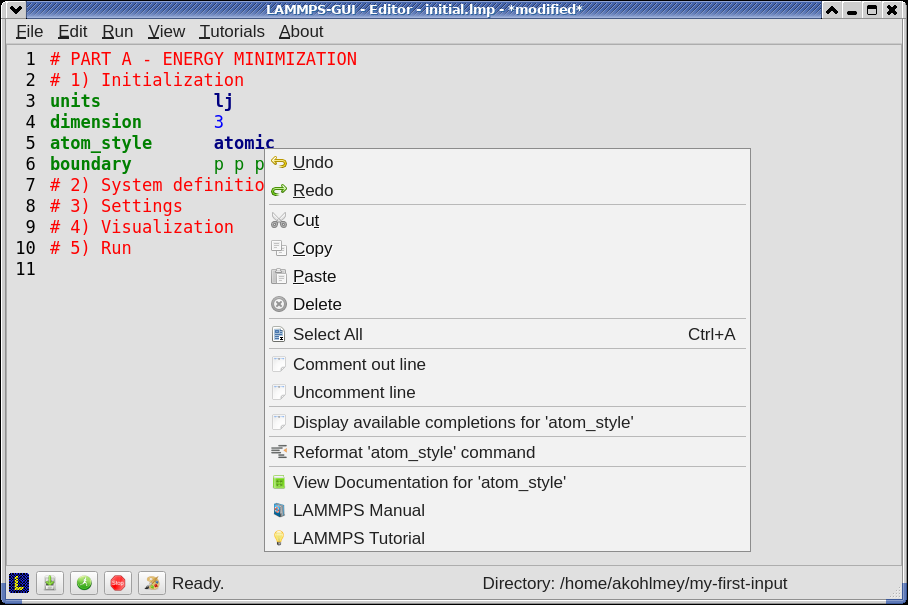
\includegraphics[width=0.75\linewidth]{GUI-1.png}
\caption{A screenshot of the LAMMPS-GUI \textit{Editor} window during
  \hyperref[lennard-jones-label]{Tutorial 1}. The coloring of the text
  is based on the syntax for LAMMPS input files.  The pop-up menu is the
  context menu for right-clicking on the ``atom\_style'' line.}
\label{fig:GUI-1}
\end{figure}

Each LAMMPS command is associated with extensive online documentation
detailing the different options for that command.  From the LAMMPS-GUI
editor buffer, the LAMMPS documentation can be accessed by
right-clicking the line with a command, such as \textit{units lj}, and
selecting \textit{View documentation for (\dots)}\,.  LAMMPS--GUI will
ask your web browser to open the corresponding URL in the online manual.
See figure \ref{fig:GUI-1} for a screenshot with such a context menu.

\paragraph{System definition}

The next step is to create the simulation box and put some atoms into it.
Modify the \textit{System definition} category of \textit{input.lmp} as follows:
{\normalsize
\begin{verbatim}
# 2) System definition
region simulation_box block &
    -20.0 20.0 -20.0 20.0 -20.0 20.0 units box
create_box 2 simulation_box
create_atoms 1 random 1500 &
    341341 simulation_box overlap 0.3
create_atoms 2 random 100 &
    127569 simulation_box overlap 0.3
\end{verbatim}
}

The first line, \textit{region simulation\_box (...)}, creates a region
named \textit{simulation\_box} that is a block (i.e. a rectangular
cuboid) that extends from -20 to 20 length units along all 3 directions
of space.  The \textit{units box} option requests that the region dimensions
are computed as multiples of the length unit and not as multiples of the
lattice spacing (\textit{units lattice}).  In this specific case there is
no difference, since we did not use the \textit{lattice} command and the
default lattice spacing is 1.0 in x-, y-, or z-direction.

The second line, \textit{create\_box 2 simulation\_box}, creates a
simulation box based on the region \textit{simulation\_box} with two
types of atoms.  From this point on, any command referencing an atom
type larger than \textit{2} will trigger an error.  You may specify more
atom types than what are necessary, but for each atom type you must set
the mass and provide force field parameters for all of them. Not doing
so will cause LAMMPS to abort with an error at the beginning of a
minimization or an MD run.

The third line, \textit{create\_atoms (\dots)}, creates 1500 atoms of type
\textit{1} at random positions within the region
\textit{simulation\_box}.  The integer \textit{341341} is a seed for the
internal random number generator that can be changed to create different
sequences of random numbers and thus different initial geometries for
the simulation.  The fourth line creates 100 atoms of type \textit{2}.
Both \textit{create\_atoms} commands use the optional argument
\textit{overlap 0.3} to add a constraint to the randomly placed atoms
that they much have at least 0.3 length units distance.  This step is to
avoid so-called ``close contacts'' between atoms which can cause
problems due to causing large forces.

\begin{figure}
\centering
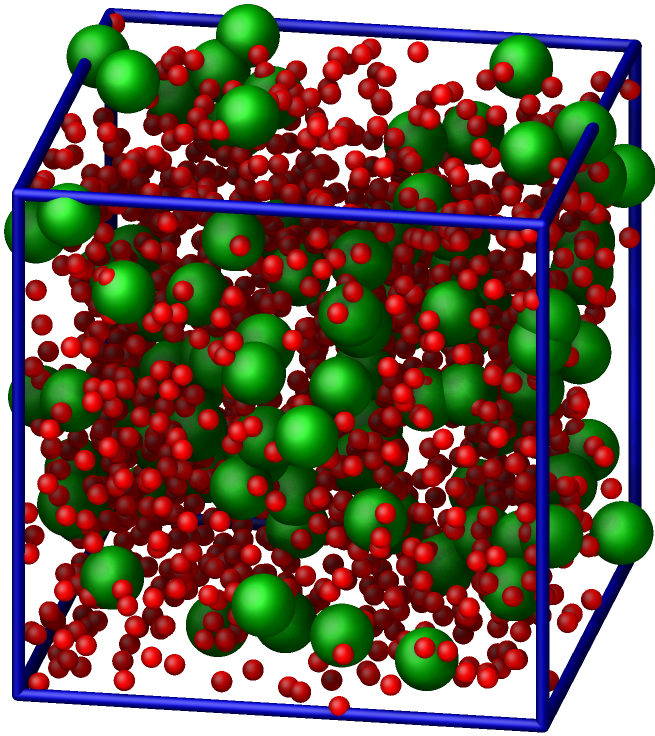
\includegraphics[width=0.55\linewidth]{LJ}
\caption{The binary mixture simulated during \hyperref[lennard-jones-label]{Tutorial 1}.
  The atoms of type 1 are represented as small red spheres, the atoms of type 2 as large
  green spheres, and the edges of the simulation box are represented a blue sticks}
\label{fig:LJ}
\end{figure}

\paragraph{Settings}
Now we provide the settings for the two types of atoms.  Modify the
\textit{Settings} category of \textit{input.lmp} as follows:
{\normalsize
\begin{verbatim}
# 3) Settings
mass 1 1.0
mass 2 1.0
pair_style lj/cut 2.5
pair_coeff 1 1 1.0 1.0
pair_coeff 2 2 0.5 3.0
\end{verbatim}
}

The two \textit{mass} commands assign a mass of 1.0 mass unit
to both atoms of type 1 and 2, respectively.  The same effect could be
achieved with a single \textit{mass * 1.0} command. The star (*) character
is a wild card representing all atom types.

The third line, \textit{pair\_style lj/cut 2.5}, requests that the atoms will
be interacting through a Lennard-Jones (LJ) potential with a cut-off equal to
$r_c = 2.5$ length units \cite{wang2020lennard,fischer2023history}:
$$E_{ij} (r) = 4 \epsilon_{ij} \left[ \left( \dfrac{\sigma_{ij}}{r} \right)^{12}
  - \left( \dfrac{\sigma_{ij}}{r} \right)^{6} \right], ~ \text{for} ~ r
< r_c,$$ where $r$ is the inter-particle distance, $\epsilon_{ij}$ is
the depth of the potential well that sets the interaction strength, and
$\sigma_{ij}$ represents the distance where the potential energy of the
LJ potential is zero.  Here, the indexes \textit{ij} refer to the
particle types \textit{i} and \textit{j}.  The minimum of the LJ
potential in this formulation is at
$\bar{\sigma} = 2^{\frac{1}{6}}\sigma$.  Sometimes people use an
alternate formulation of the LJ potential which uses $\bar{\sigma}$,
i.e. the minimum of the potential.  By substituting
$\sigma = \frac{\bar{\sigma}}{2^{\frac{1}{6}}}$ in the formulation above
we get the alternate but equivalent expression:
$$E_{ij} (r) = \epsilon_{ij} \left[ \left( \dfrac{\bar{\sigma}_{ij}}{r} \right)^{12}
  - 2\left( \dfrac{\bar{\sigma}_{ij}}{r} \right)^{6} \right], ~
\text{for} ~ r < r_c,$$ LAMMPS can run simulations for both formulations
with the same \textit{lj/cut} pair style, only the parameters for $\bar{\sigma}$
of the second formulation must be divided by $2^{\frac{1}{6}}$ to get the $\sigma$
needed for the first formulation for the LJ potential.

The fourth line, \textit{pair\_coeff 1 1 1.0 1.0}, sets the
Lennard-Jones coefficients for the interactions between pairs of atoms
of type 1, respectively the energy parameter $\epsilon_{11} = 1.0$ and
the distance parameter $\sigma_{11} = 1.0$.  Similarly, the last line
sets the Lennard-Jones coefficients for the interactions between atoms
of type 2, $\epsilon_{22} = 0.5$, and $\sigma_{22} = 3.0$.  By default,
LAMMPS calculates the cross coefficients between the different atom
types using geometric average:
$\epsilon_{ij} = \sqrt{\epsilon_{ii} \epsilon_{jj}}$,
$\sigma_{ij} = \sqrt{\sigma_{ii} \sigma_{jj}}$.  In the present case, we
thus have: $\epsilon_{12} = \sqrt{1.0 \times 0.5} = 0.707$, and
$\sigma_{12} = \sqrt{1.0 \times 3.0} = 1.732$.

\paragraph{Energy minimization}
The system is now fully parameterized and the input ready to compute
forces.  Let us fill in the two last remaining categories,
\textit{Visualization}, and \textit{Run}, by adding the following lines
into \textit{input.lmp}:
{\normalsize
\begin{verbatim}
# 4) Visualization
thermo 10
thermo_style custom step etotal press

# 5) Run
minimize 1.0e-6 1.0e-6 1000 10000
\end{verbatim}
}
The \textit{thermo} command asks LAMMPS to print thermodynamic
information to the console every given number of steps, in this
input every 10 simulation steps.  The \textit{thermo\_style custom} determines
\emph{which} output LAMMPS should print.  This selection prints the
the step number (\textit{step}), the total energy (\textit{etotal}), and the
pressure (\textit{press}).

Finally, the \textit{minimize} command tells LAMMPS to perform an energy
minimization of the system.  That is, LAMMPS will compute the forces on
all atoms and then update the positions according to a selected
algorithm so that the potential energy will decrease.  By default,
LAMMPS uses the conjugate gradient (CG) algorithm
\cite{hestenes1952methods}.  The simulation will stop as soon at the
minimizer algorithm cannot find a way to to lower the potential energy.
Except for trivial systems, minimization algorithms will find the
``next'' minimum, which may not be the global minimum.

Now you can run the simulation by selecting \textit{Run LAMMPS from Editor
  Buffer} from the \textit{Run} menu, or by using the
\texttt{Ctrl-Enter} keyboard shortcut or by clicking on the green ``Run
LAMMPS'' button (second from left) in the status bar.  The simulation
can be stopped at any time by using \textit{Stop LAMMPS} from the
\textit{Run} menu, the \texttt{Ctrl-/} keyboard shortcut or by clicking
on the red stop button in the status bar.  A new run will always
``forget'' the current system and start over from the top.

\begin{figure}
\centering
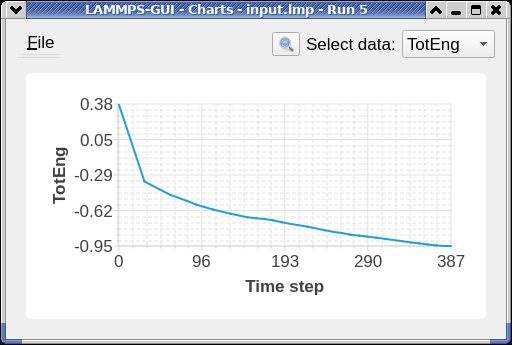
\includegraphics[width=0.45\linewidth]{chart-1}
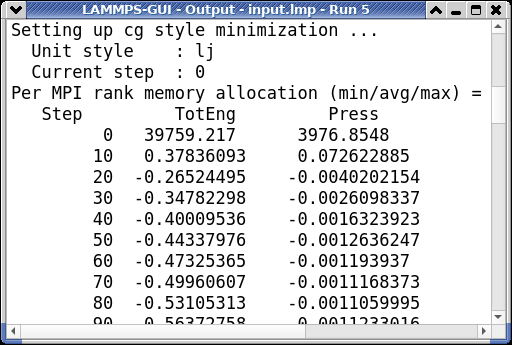
\includegraphics[width=0.45\linewidth]{output-1}
\caption{\textit{Chart} (left) and \textit{Output} (right) window of LAMMPS-GUI after performing
  the minimization simulation of \hyperref[lennard-jones-label]{Tutorial 1}.}
\label{fig:chart-log}
\end{figure}

As the simulation launches, two additional windows will show up as shown
in figure \ref{fig:chart-log}: a \textit{Charts} window showing the
evolution of the total energy and an \textit{Output} window with the
output LAMMPS writes to the console during a simulation. This includes
the thermodynamic data in text form that is plotted in the \textit{Chart} window.

If the plot in your \textit{Chart} window is missing data, your
computer is running the simulation too fast for LAMMPS--GUI to collect
all the data.  You can adjust the settings in the
\textit{Edit~$\to$~Preferences} dialog to collect data more frequently
by reducing the \textit{GUI update interval}.  At values lower
than 10\,ms, the time the GUI spends on collecting the data becomes
significant and thus such settings should only be used for fast tutorials like
this one.  You can also make your simulation slower by selecting
\textit{None} in the \textit{Accelerators} tab.

The potential energy can be seen to decrease from a positive value to a
negative value.  The initially positive value of the potential energy is
expected because the atoms have been created at random positions within
the simulation box and some of them are very close, resulting in a large
initial potential energy due to the repulsive branch of the
Lennard-Jones potential.  As the energy minimization progresses, the
energy decreases -- first rapidly -- then more slowly and plateaus at
a negative value, indicating that the atoms have been displaced to
reasonable distances from each other.

Since the \textit{thermo\_style} command also includes the output of the
pressure, it is possible to switch from plotting the total energy to
showing the pressure by choosing \textit{Press} in \textit{Select data}
drop down menu.

\paragraph{Snapshot Image}

At this point it is also possible to create a snapshot image of the
current system using the \textit{Image Viewer} window.  To open it, use
either \textit{Create Image} from the \textit{Run} menu, the
\texttt{Ctrl-I} keyboard shortcut, or by clicking on the (right) palette
button in the status bar.  The image viewer works by telling LAMMPS to
render an image of the current system using its own render library
through the \textit{dump image} command and then reading in and
displaying the created image.  The various buttons can be used to change
what is shown and how it is rendered.  The image of figure \ref{fig:LJ}
was created this way.  To see a snapshot of the system at the beginning
of the run, you can temporarily replace the \textit{minimize} command
with \textit{run 0}.  This will perform one force iteration in LAMMPS without
moving atoms to initialize the system.

\paragraph{Molecular dynamics}

After the energy minimization, any overlapping atoms have been displaced,
and the system is now ready to perform a molecular dynamics simulation
using the minimized geometry.  Since we want to start from the result of
the energy minimization step, we can append commands for the MD simulation
to the same input script, \textit{input.lmp}. After the
\textit{minimize} command, add the following lines:
{\normalsize
\begin{verbatim}
# PART B - MOLECULAR DYNAMICS
# 4) Visualization
thermo 50
thermo_style custom step temp etotal &
    pe ke press
\end{verbatim}
}

Since LAMMPS reads the input from top to bottom and acts on each line
immediately, these lines will be executed \emph{after} the energy
minimization.  There is no need to re-initialize or re-define the
system.  The \textit{thermo} command is called a second time to change
the previous value of 10 to a value of 50 as soon as \textit{PART B} of
the simulation starts.  In addition, a new \textit{thermo\_style}
command changes which thermodynamic information to be printed by LAMMPS
during \textit{PART B}.  This is done because, during molecular
dynamics, the system will have a non-zero temperature (\textit{temp})
and kinetic energy (\textit{ke}) and it is useful to monitor those.
Here, \textit{pe} is the potential energy of the system, such that
\textit{pe + ke = etotal}.

Then, let us add a second \textit{Run} category by adding the following
lines to \textit{PART B} of \textit{input.lmp}:
{\normalsize
\begin{verbatim}
# 5) Run
fix mynve all nve
timestep 0.005
run 10000
\end{verbatim}
}
The \textit{fix nve} command is used to update the positions and the
velocities of the atoms in the group \textit{all} at every step.  The
group \textit{all} is a default group that contains every atom.  The
last two lines set the value of the \textit{timestep} and the number of
steps for the \textit{run}, respectively, corresponding to a total
duration of 50 time units.

Since there are no other fix commands that change forces or velocities,
and since we have periodic boundary conditions in all directions, the MD
simulation will be performed in the microcanonical or NVE ensemble.
This means the system has no exchange of energy outside the simulation
box and the number of particles and the box volume are constant.  We can
see that there is no equilibrium between potential and kinetic energy
yet, as the former is falling while the latter is rising.  If you extend
the run for many more steps, the values for both kinetic and
potential energy will plateau (indicating equilibrium) and the total
energy should fluctuate around some constant value.  To achieve the
latter, we have to reduce errors by increasing the cutoff to 5 length
units and reducing the timestep to 0.0025 time units since the choices
of 2.5 and 0.005 are quite aggressive.

Now we change the \textit{Run} section to:
{\normalsize
\begin{verbatim}
# 5) Run
fix mynve all nve
fix mylgv all langevin 1.0 1.0 0.1 1530917
timestep 0.005
run 10000
\end{verbatim}
}

The new command adds a ``Langevin thermostat'' to the atoms in the group
\textit{all}, with a desired target temperature of 1.0 temperature units
throughout the run (the two numbers stand for the target at the beginning
and at the end of the run, which allows for a temperature ramp if
they differ) \cite{schneider1978molecular}.  A \textit{damping}
parameter of 0.1 is used.  The \textit{damping} parameter determines how
rapidly the temperature is relaxed to its desired value.  In a Langevin
thermostat the atoms are subject to friction and random noise (in the form
of randomly added velocities).  Since a constant friction term removes
more kinetic energy from fast atoms and less from slow atoms, the system
will eventually reach a dynamic equilibrium where the kinetic energy
removed and added are about the same.  The number \textit{1530917} is a
seed used to initialize the random number generator used inside of
\textit{fix langevin}, you can change it to perform statistically
independent simulations.

Run the simulation again using LAMMPS. Open the \textit{Output} window
by selecting \textit{View}, and \textit{Output}. From the information
printed in the \textit{Output} window, one can see that the temperature
\textit{Temp} starts from 0, but rapidly reaches the requested value and
stabilizes itself near $T=1$ temperature units.  One can also see that
the potential energy, $p_\text{e}$, rapidly decreases during energy
minimization (see also Fig.\,\ref{fig:evolution-energy}\,a). After
the molecular dynamics simulation starts, $p_\text{e}$ increases until
it reaches a plateau value of about -0.25. The kinetic energy,
$k_\text{e}$, is equal to zero during energy minimization and then
increases during molecular dynamics until it reaches a plateau value of
about 1.5 (Fig.\,\ref{fig:evolution-energy}\,b).

\begin{figure}
\centering
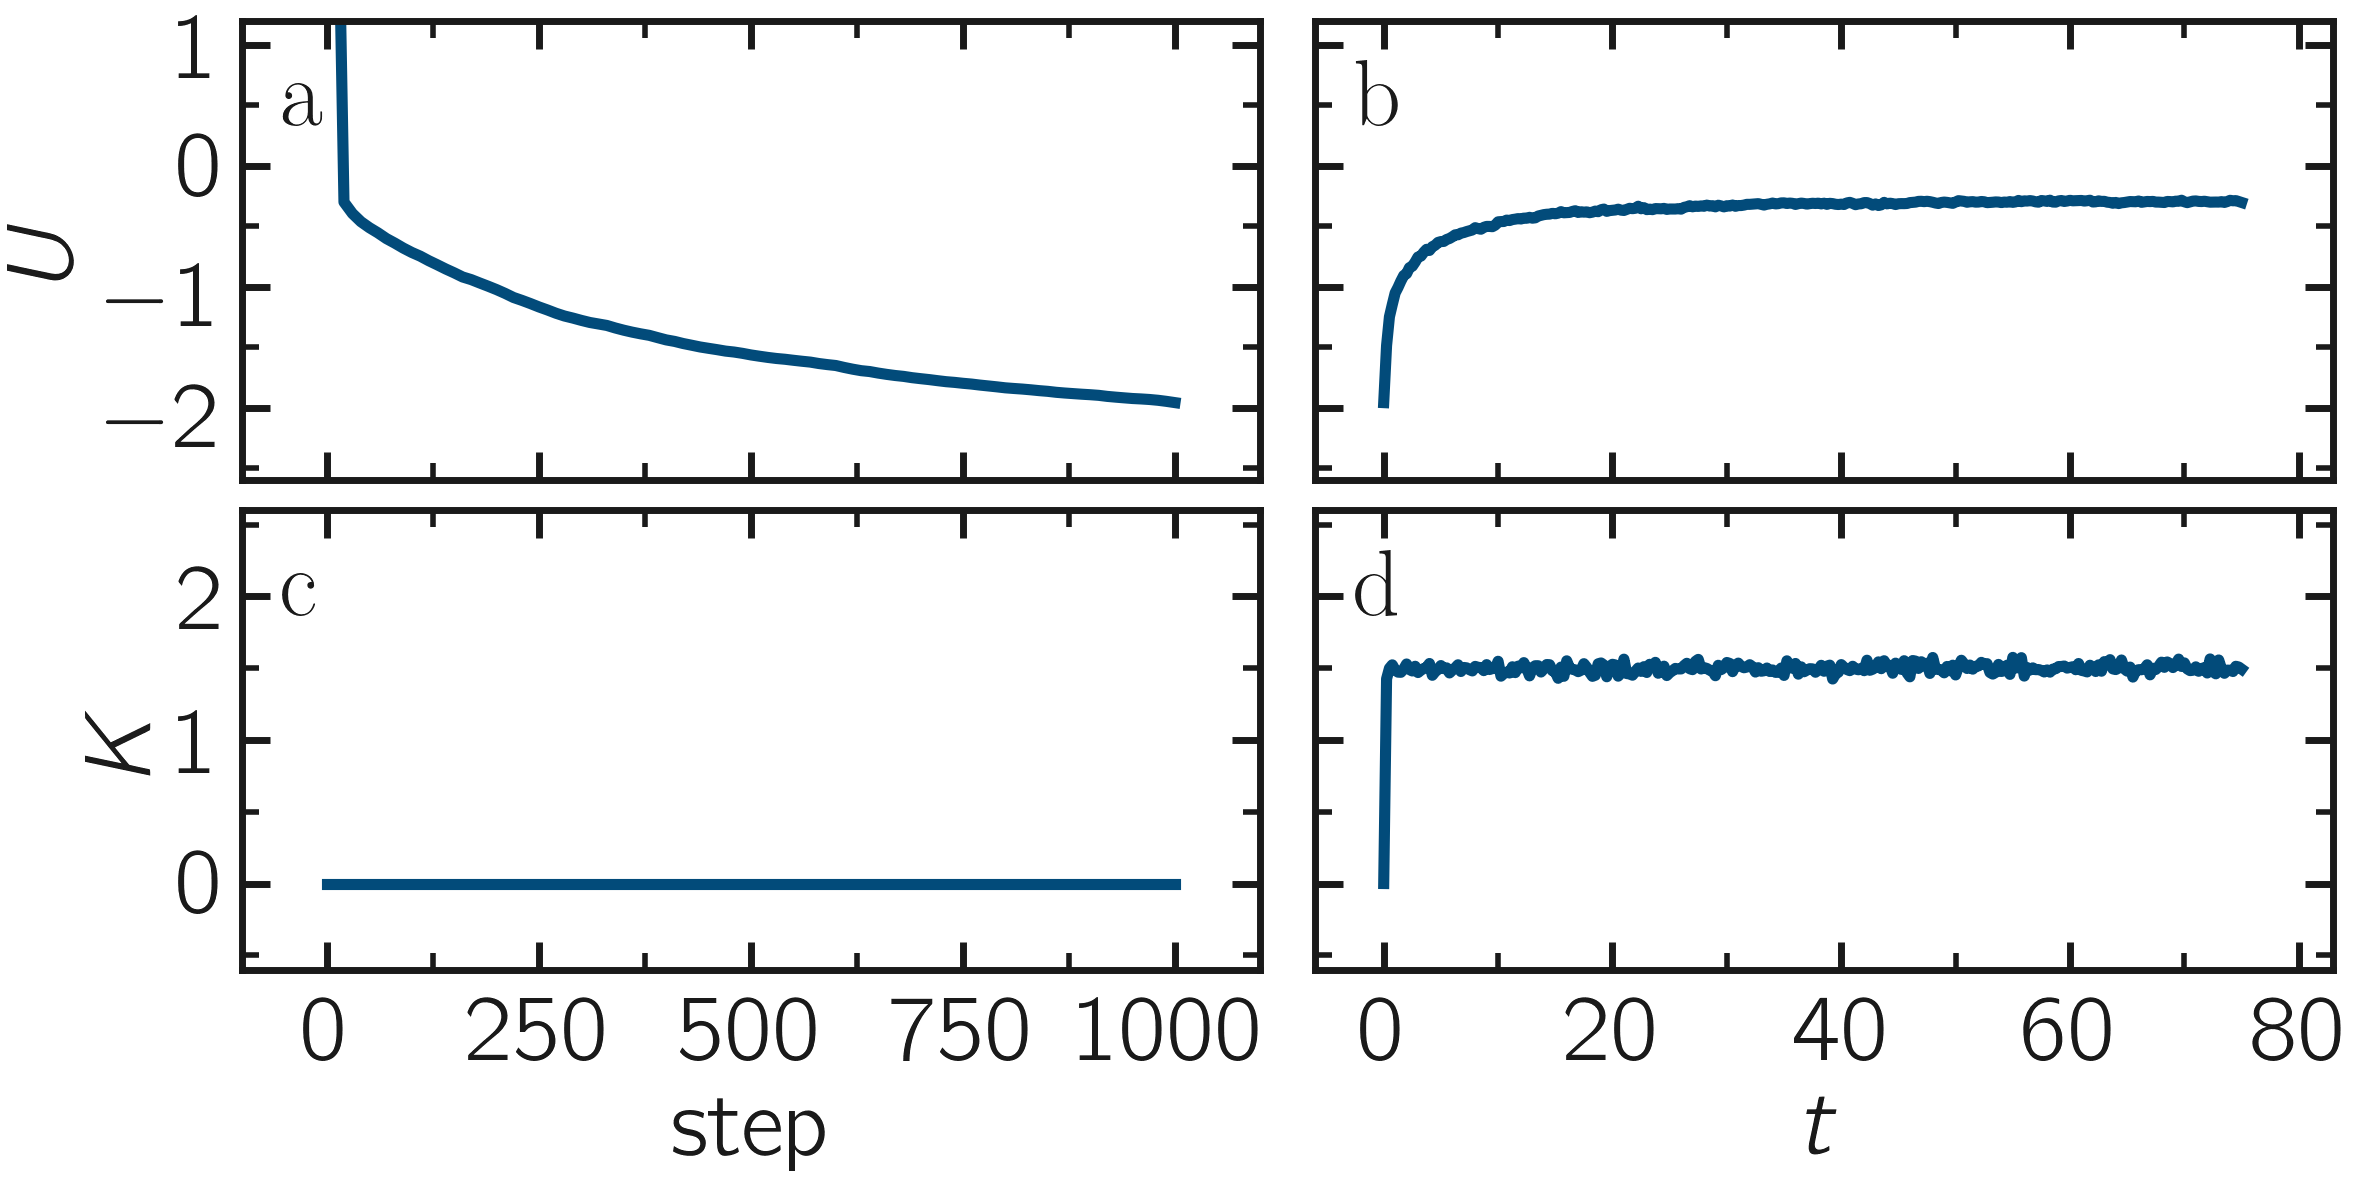
\includegraphics[width=\linewidth]{LJ-energy}
\caption{a) Potential energy ($p_\text{e}$) of the binary mixture as a function
of the time $t$. b) Kinetic energy ($k_\text{e}$) as a function of $t$.}
\label{fig:evolution-energy}
\end{figure}

\paragraph{Trajectory visualization}

So far, the simulation was monitored only from the thermodynamic
information.  To better follow the evolution of the system and visualize
the trajectories of the atoms, we use the \textit{dump image} command to
create snapshot images during the simulation.  We have already explored
the \textit{Image Viewer} window.  Open it (again) and adjust the
visualization to your liking using the various buttons.  Now you can
copy the command line used to create this visualization to the clipboard
by either using the \texttt{Ctrl-D} keyboard shortcut or select
\textit{Copy dump image command} from the \textit{File} menu.  This text
can be pasted into the into the \textit{Visualization} section of
\textit{PART B:} of the \textit{input.lmp} file.

This may look like the following:
{\normalsize
\begin{verbatim}
dump viz all image 100 myimage-*.ppm type type size 800 800 &
    zoom 1.452 shiny 0.5  fsaa yes view 80 10 box yes 0.025 &
    axes no 0.0 0.0 center s 0.483725 0.510373 0.510373
dump_modify viz pad 9 boxcolor darkblue backcolor white &
    adiam 1 1.6 adiam 2 4.8
\end{verbatim}
}
This command tells LAMMPS to generate NetPBM format images every 100
steps. The two \textit{type} keywords are for \textit{color} and
\textit{diameter}, respectively.  Run the \textit{input.lmp} using
LAMMPS again, and a new window named \textit{Slide Show} will pop up.
It will show each image created by the \textit {dump image} as it is
created and after the simulation is finished (or stopped), the slide
show viewer allows to animate the trajectory by cycling through the
images.  The window also allows to export the animation to a movie
(provided the FFMpeg program is installed) and to bulk delete those
image files.

The rendering of the system can be further adjusted using the many
options of the \textit{dump image} command.  The value for the
\textit{shiny} keyword is used to adjust the shininess of the atoms, the
\textit{box} keyword adds or removes a representation of the box, and
the \textit{view} and \textit{zoom} keywords adjust the camera and so
on.

\subsubsection{Improving the script}

Let us improve the input script and perform slightly more advanced operations,
such as imposing specific initial positions on the atoms and restarting the
simulation from a previously saved configuration.

\paragraph{Control the initial atom positions}
Create a new folder next to \textit{my-first-input/} and call it
\textit{improved-input/}. Then, create a new input file within
\textit{improved-input/} and call it \textit{input.min.lmp}. Similarly to what
has been done previously, copy the following lines into \textit{input.min.lmp}:
{\normalsize
\begin{verbatim}
# 1) Initialization
units lj
dimension 3
atom_style atomic
pair_style lj/cut 2.5
boundary p p p
\end{verbatim}
}
To create the atoms of types 1 and 2 in two separate regions, let us create
three separate regions: a cubic region for the simulation box and two additional
regions for placing the atoms:
{\normalsize \begin{verbatim}
# 2) System definition
region simulation_box block &
    -20 20 -20 20 -20 20
create_box 2 simulation_box
region cylinder_in cylinder z 0 0 10 &
    INF INF side in
region cylinder_out cylinder z 0 0 10 &
    INF INF side out
create_atoms 1 random 1000 341341 cylinder_out
create_atoms 2 random 150 127569 cylinder_in
\end{verbatim}}
The \textit{side in} and \textit{side out} keywords are used to define regions
that are respectively inside and outside of the cylinder of radius 10. Then,
copy similar lines as previously into \textit{input.min.lmp}:
{\normalsize \begin{verbatim}
# 3) Settings
mass 1 1
mass 2 1
pair_coeff 1 1 1.0 1.0
pair_coeff 2 2 0.5 3.0

# 4) Visualization
thermo 10
thermo_style custom step etotal press
dump mydmp all image 100 dump.min.*.jpg &
    type type shiny 0.1 box no 0.01 &
    view 0 0 zoom 1.8
dump_modify mydmp acolor 1 darkturquoise &
    acolor 2 darkblue adiam 1 1 adiam 2 3 &
    backcolor white

# 5) Run
minimize 1.0e-4 1.0e-6 1000 10000
write_data minimized_coordinate.data
\end{verbatim}}
The main novelty, compared to the previous input script, is the \textit{write\_data}
command. This command is used to print the final state of the simulation in a file
called \textit{minimized\_coordinate.data}. Note that the \textit{write\_data}
command is placed after the \textit{minimize} command. This \textit{.data} file
will be used later to restart the simulation from the final state of the energy
minimization step.

Run the \textit{input.min.lmp} script using LAMMPS. At the end of the simulation,
a file called \textit{minimized\_coordinate.data} is created by LAMMPS. If you
open \textit{minimized\_coordinate.data} with a text editor, you can see that
it contains all the information necessary to restart the simulation, such as the
number of atoms, the box size, the \textit{masses}, and the \textit{pair\_coeffs}.
The \textit{minimized\_coordinate.data} file also contains the final positions
of the atoms within the \textit{Atoms} section. The first five columns of the
\textit{Atoms} section correspond (from left to right) to the atom indexes (from
1 to the total number of atoms, 1150), the atom types (1 or 2 here), and the
positions of the atoms $x$, $y$, $z$. The last three columns are image flags
that keep track of which atoms crossed the periodic boundary.

\paragraph{Restarting from a saved configuration}

Let us create a new input file and start a molecular dynamics simulation
directly from the previously saved configuration. Within \textit{improved-input/},
create a new file called \textit{input.md.lmp} and copy the same lines as previously:
{\normalsize \begin{verbatim}
# 1) Initialization
units lj
dimension 3
atom_style atomic
pair_style lj/cut 2.5
boundary p p p
\end{verbatim}}
Here, instead of creating a new region and adding atoms to it, we can simply
import the previously saved configuration by adding the following command to
\textit{input.md.lmp}:
{\normalsize \begin{verbatim}
# 2) System definition
read_data minimized_coordinate.data
\end{verbatim}}
By visualizing the system using the generated JPG images, you may have noticed
that some atoms have moved from one region to the other during minimization.
To start the simulation from a clean slate, with only atoms of type 2 within the
cylinder and atoms of type 1 outside the cylinder, let us delete the misplaced
atoms by adding the following commands to \textit{input.md.lmp}:
{\normalsize \begin{verbatim}
region cylinder_in cylinder z 0 0 10 &
    INF INF side in
region cylinder_out cylinder z 0 0 10 &
    INF INF side out
group group_type_1 type 1
group group_type_2 type 2
group group_region_in region cylinder_in
group group_region_out region cylinder_out
group group_type_1_in &
    intersect group_type_1 group_region_in
group group_type_2_out &
    intersect group_type_2 group_region_out
delete_atoms group group_type_1_in
delete_atoms group group_type_2_out
\end{verbatim}}
The two first \textit{region} commands recreate the previously defined regions,
which is necessary since regions are not saved by the \textit{write\_data}
command. The first two \textit{group} commands are used to create groups containing
all the atoms of type 1 and all the atoms of type 2, respectively. The next two
\textit{group} commands create atom groups based on their positions at the beginning
of the simulation, i.e. when the commands are being read by LAMMPS. The last two
\textit{group} commands create atom groups based on the intersection between the
previously defined groups. Finally, the two \textit{delete\_atoms} commands delete
the atoms of type 1 that are located within the cylinder and the atoms of type 2
that are located outside the cylinder, respectively.

Let us measure the number of atoms of each type inside the cylinder as a function
of time, by creating the following variables:
{\normalsize \begin{verbatim}
variable n1_in &
    equal count(group_type_1,cylinder_in)
variable n2_in &
    equal count(group_type_2,cylinder_in)
\end{verbatim}}
The two \textit{variables} are used to count the number of atoms of a specific
group in the \textit{cylinder\_in} region.

In addition to counting the atoms in each region, let us also extract the
coordination number per atom between atoms of types 1 and 2. The coordination
number is a measure of the average number of type 2 atoms in the vicinity of
type 1 atoms, which serves as a good indicator of the degree of mixing in a
binary mixture. Add the following lines into \textit{input.md.lmp}:
{\normalsize \begin{verbatim}
compute coor12 group_type_1 coord/atom &
    cutoff 2.0 group group_type_2
compute sumcoor12 all reduce ave c_coor12
\end{verbatim}}
The \textit{compute ave} is used to average the per atom coordination number
that is calculated by the \textit{coord/atom} compute.

Add the following lines into \textit{input.md.lmp}. Note the absence of
\textit{Settings} section, because the settings are taken from the \textit{.data} file.
{\normalsize \begin{verbatim}
# 4) Visualization
thermo 1000
thermo_style custom step temp pe ke etotal &
    press v_n1_in v_n2_in c_sumcoor12

dump mydmp all image 100 dump.md.*.jpg &
    type type shiny 0.1 box no 0.01 &
    view 0 0 zoom 1.8
dump_modify mydmp acolor 1 darkturquoise &
    acolor 2 darkblue adiam 1 1 adiam 2 3 &
    backcolor white
\end{verbatim}}
The two variables, \textit{n1\_in}, \textit{n2\_in}, and the
compute \textit{sumcoor12}, were added to the list of information printed during
the simulation.

\begin{figure}
\centering
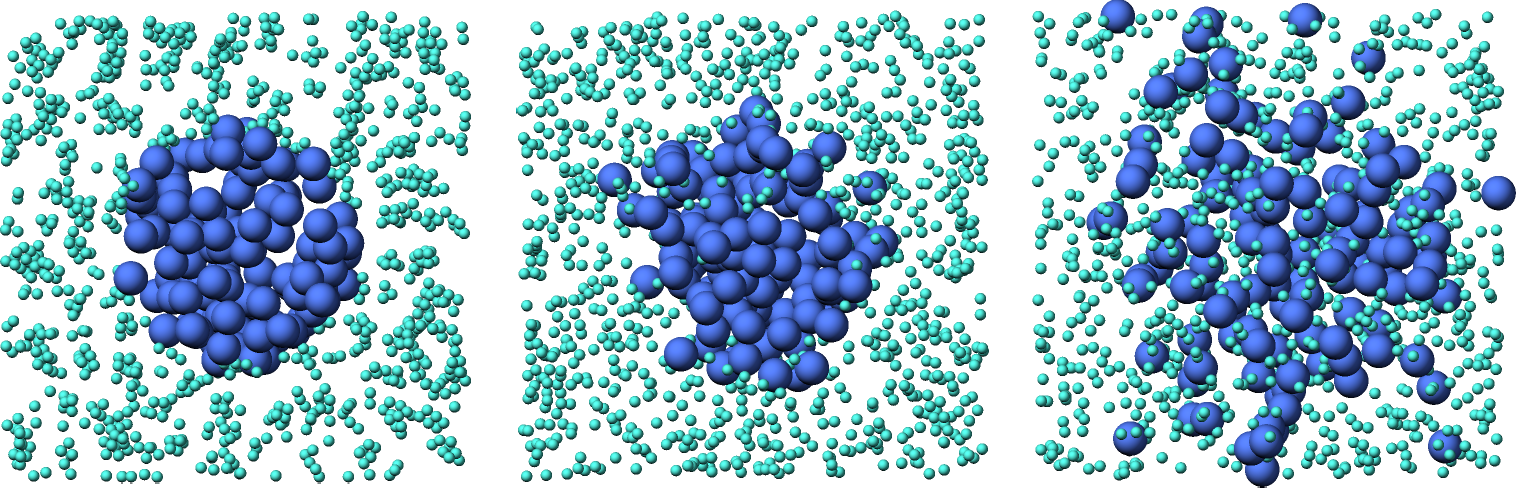
\includegraphics[width=\linewidth]{LJ-evolution}
\caption{Evolution of the system during mixing. The three snapshots show
respectively the system at $t=0$ (left panel), $t=75$ (middle panel), and $t=1500$
(right panel).}
\label{fig:evolution-population}
\end{figure}

Finally, let us complete the script by adding the following lines into \textit{input.md.lmp}:
{\normalsize \begin{verbatim}
# 5) Run
velocity all create 1.0 4928459 &
    mom yes rot yes dist gaussian
fix mynve all nve
fix mylgv all langevin 1.0 1.0 0.1 &
    1530917 zero yes
timestep 0.005
run 300000
\end{verbatim}}
There are a few differences from the previous simulation. First, the
\textit{velocity create} command attributes an initial velocity to each atom.
The initial velocity is chosen so that the average initial temperature is equal
to 1 (unitless). The additional keywords ensure that no linear momentum
(\textit{mom yes}) and no angular momentum (\textit{rot yes}) are given to the
system and that the generated velocities are distributed as a Gaussian. Another
improvement is the \textit{zero yes} keyword in the Langevin thermostat, which
ensures that the total random force applied to the atoms is equal to zero.

Run \textit{input.md.lmp} using LAMMPS, and observe the mixing of the two
populations over time (see also Fig.\,\ref{fig:evolution-population}). From the
variables \textit{n1\_in} and \textit{n2\_in}, one can follow the number of
atoms in each region as a function of time (Fig.\,\ref{fig:mixing}\,a). In addition,
as the mixing progresses, the coordination number between atoms of types 1 and 2 increases
from about $0.01$ to $0.35$ (Fig.\,\ref{fig:mixing}\,b). This indicates that,
over time, more and more particles of type 1 come into contact with
particles of type 2, as expected during mixing.

\begin{figure}
\centering
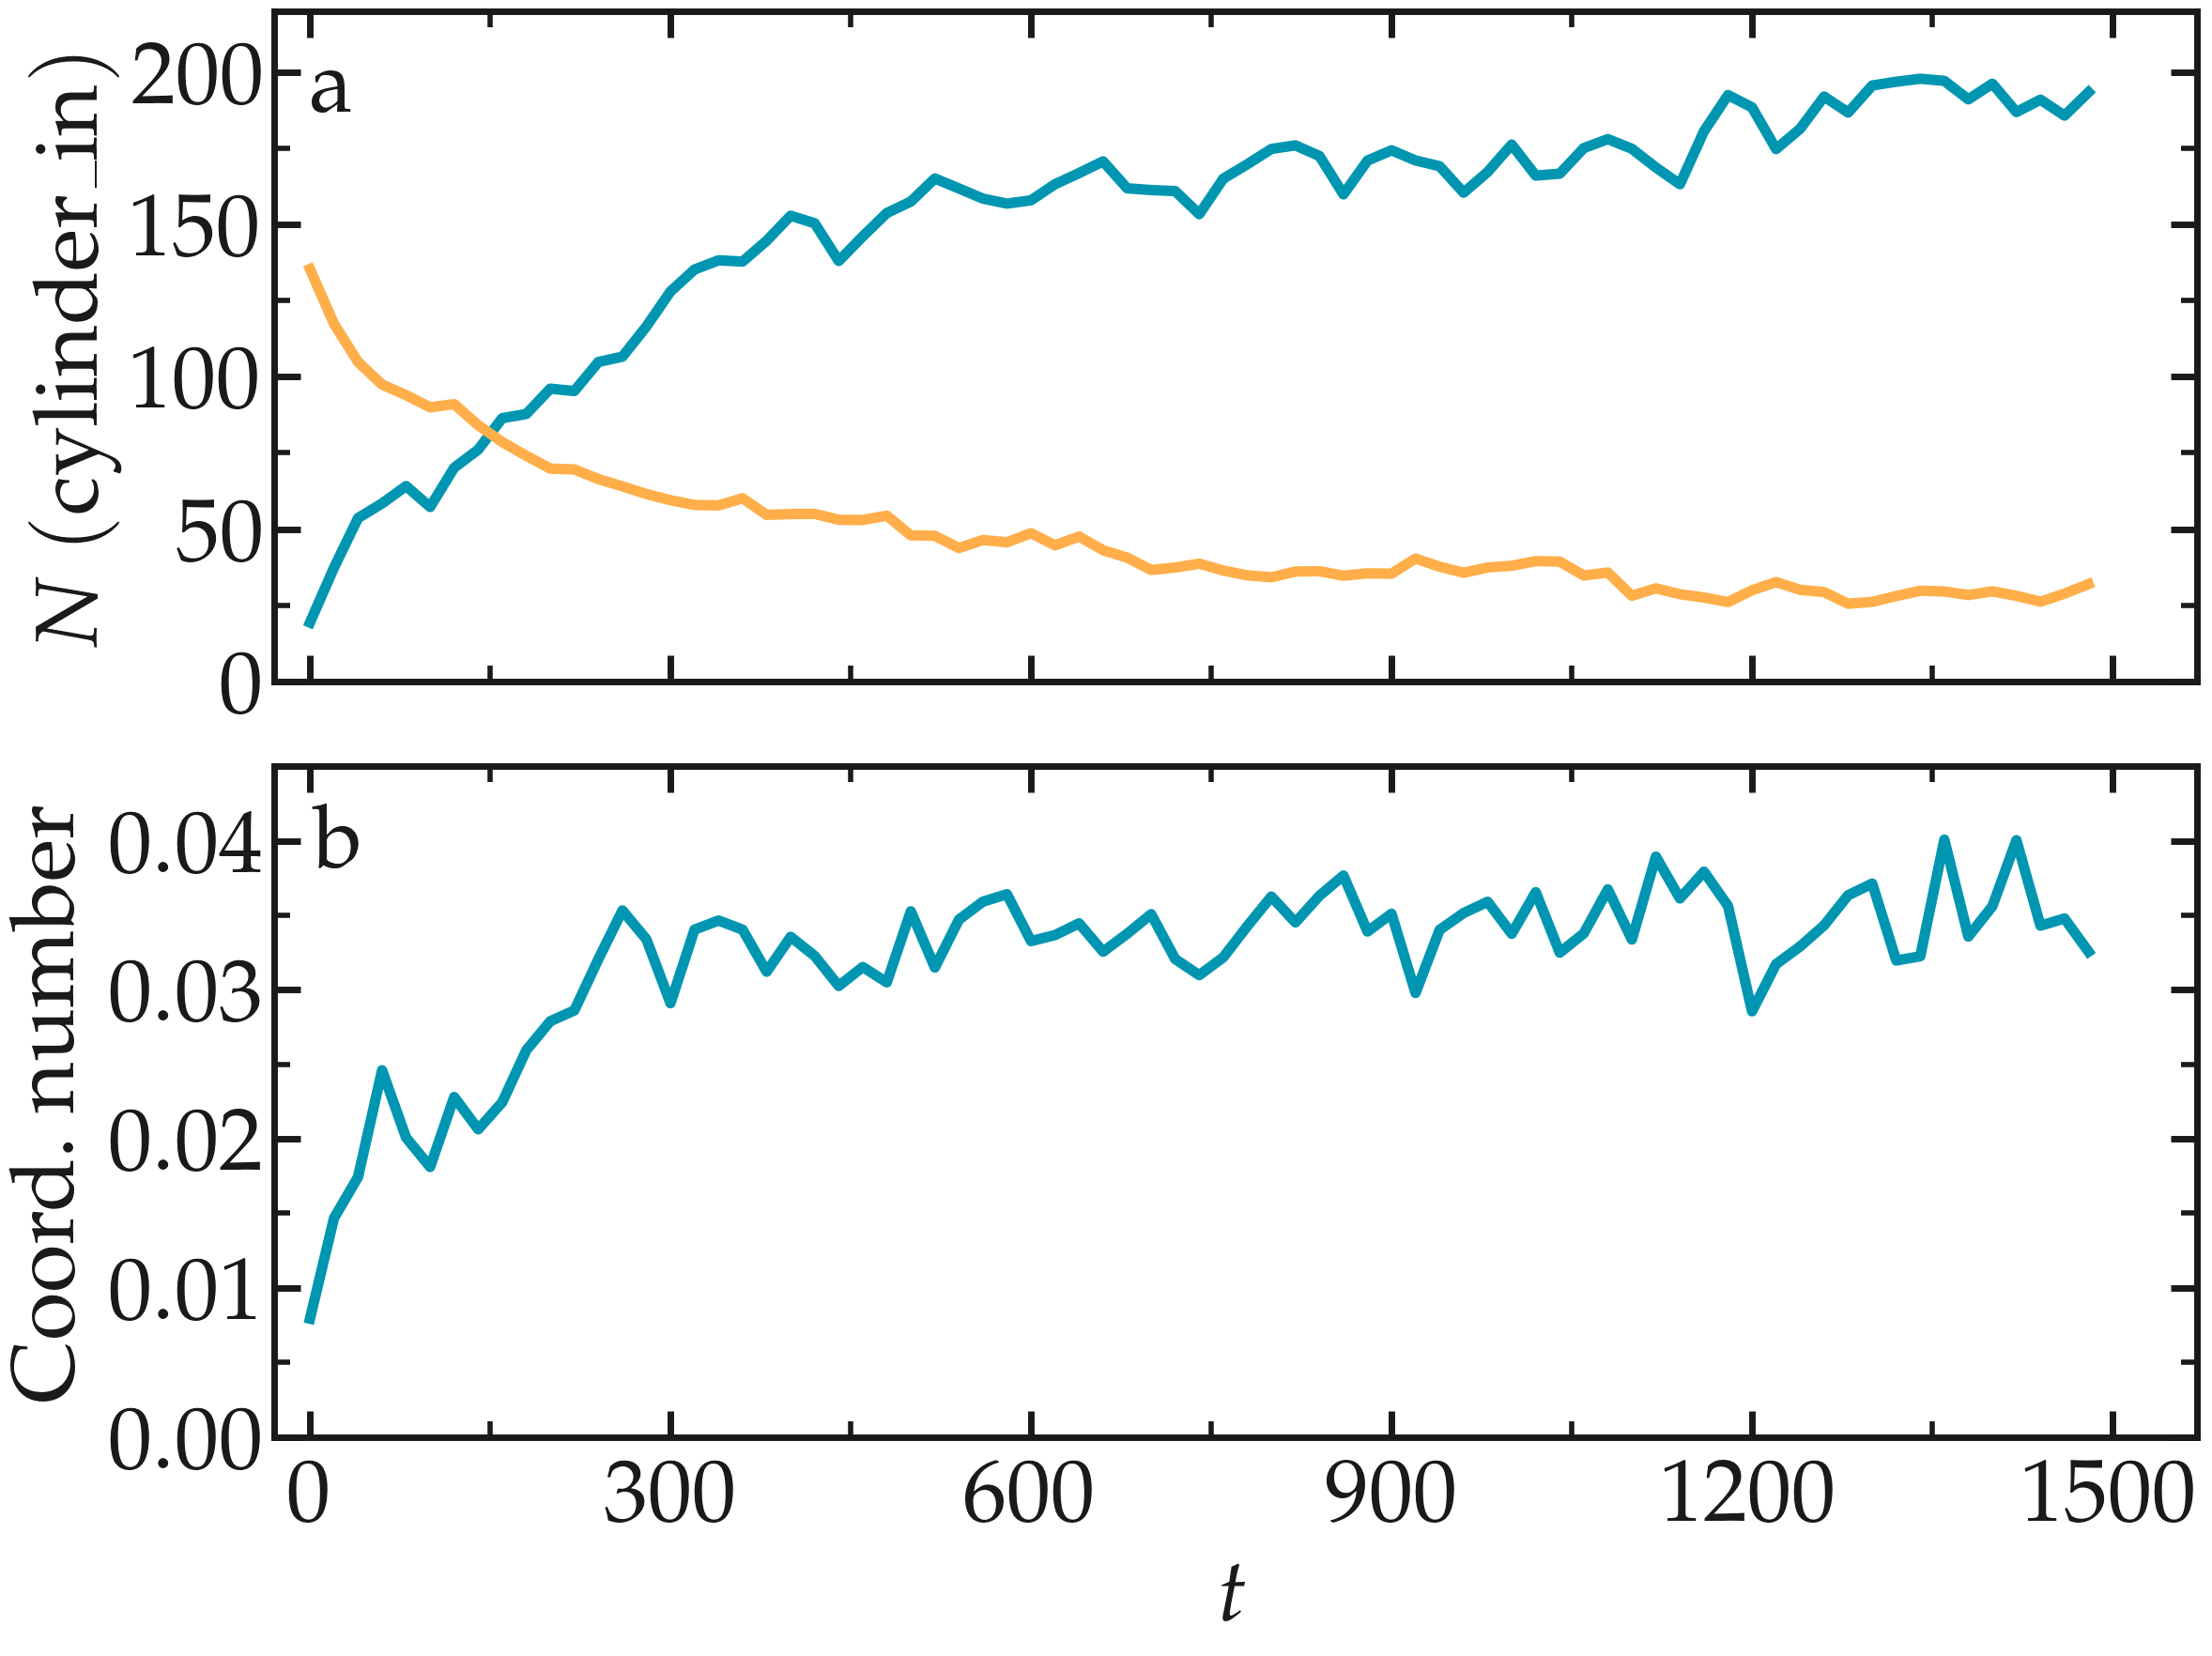
\includegraphics[width=\linewidth]{LJ-mixing}
\caption{a) Evolution of the number $N_\text{in}$ of atoms within the
\textit{cylinder\_in} region as a function of the time $t$. b) Evolution of
the coordination number $C_{1-2}$ between atoms of types 1 and 2.}
\label{fig:mixing}
\end{figure}

\subsection{Tutorial 2: Pulling on a carbon nanotube}
\label{carbon-nanotube-label}

In this tutorial, the system of interest is a small carbon nanotube
(CNT) in an empty box (Fig.\,\ref{fig:CNT}). An external force is imposed on
the CNT, and its deformation is measured over time. To illustrate the
difference between classical and reactive force fields, this tutorial is
divided into two parts. Within the first part, a classical force field is
used and the bonds between the atoms of the CNT are unbreakable. Within the
second part, a reactive force field (named AIREBO \cite{stuart2000reactive})
is used, allowing for the breaking of chemical bonds when the CNT undergoes
strong deformation.

\begin{figure}
\centering
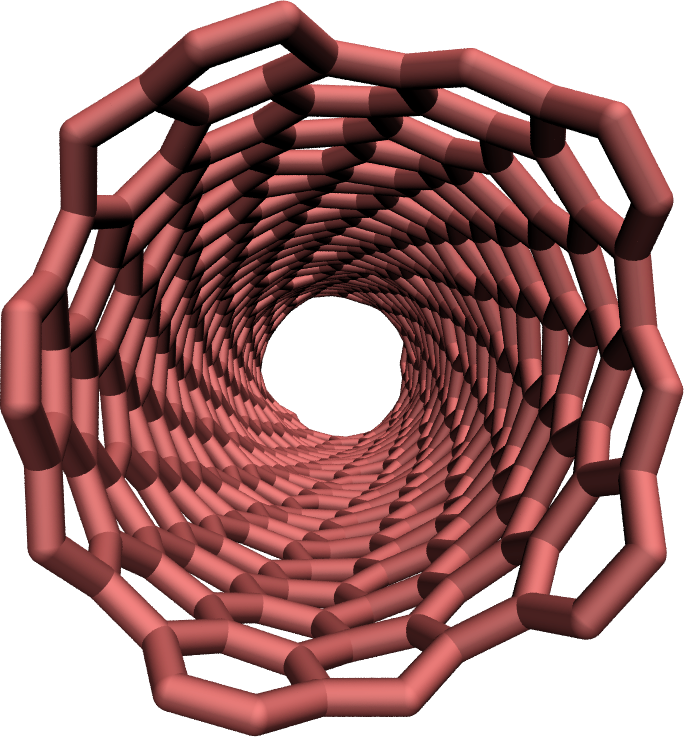
\includegraphics[width=0.55\linewidth]{CNT}
\caption{The carbon nanotube (CNT) simulated during
\hyperref[carbon-nanotube-label]{Tutorial 2}.}
\label{fig:CNT}
\end{figure}

\subsubsection{Unbreakable bonds}
With most classical molecular dynamics force fields, the chemical
bonds between the atoms are set at the start of the simulation. Regardless
of the forces applied to the atoms, the bonds remain unchanged during the
simulation. The bonds between neighbor atoms typically consist of springs
with given equilibrium distances $r_0$ and a constant
$k_\text{b}$: $U_\text{b} = k_\text{b} \left( r - r_0 \right)^2$. Additionally, angular and dihedral
constraints are usually applied to maintain the relative orientations of
neighboring atoms.

First, download the CNT topology
\href{\filepath tutorial2/unbreakable-bonds/cnt_molecular.data}{\textit{cnt\_molecular.data}}.
It was created using VMD and TopoTools \cite{kohlmeyer2017topotools}, and contains
information about the positions of the carbon atoms, as well as the identity of
the atoms that are linked by \textit{bonds}, \textit{angles}, \textit{dihedrals},
and \textit{impropers} constraints. Save the \textit{cnt\_molecular.data} file
in a folder called \textit{unbreakable-bonds/}.

\paragraph{The LAMMPS input}
Create a new text file within \textit{unbreakable-bonds/} and name
it \textit{input.lmp}. Open \textit{input.lmp} using the LAMMPS-GUI, and copy
the following lines into it:
{\normalsize \begin{verbatim}
variable T equal 300

units real
atom_style molecular
boundary f f f
pair_style lj/cut 14

bond_style harmonic
angle_style harmonic
dihedral_style opls
improper_style harmonic

special_bonds lj 0.0 0.0 0.5

read_data cnt_molecular.data
\end{verbatim}}
The chosen unit system is \textit{real} (therefore distances are in Ångstrom
and time in femtosecond), the \textit{atom\_style} is molecular (therefore
atoms are dots that can be bonded with each other), and the boundary conditions
are fixed. The boundary conditions do not matter here, as the box boundaries
were placed far from the CNT. Just like in the previous tutorial,
\hyperref[lennard-jones-label]{Lennard-Jones fluid}, the pair style
is \textit{lj/cut} (i.e. a Lennard-Jones potential with a short-range cutoff)
with parameter 14, which means that only the atoms closer than 14 Ångstroms
from each other interact through a Lennard-Jones potential.
The \textit{bond\_style}, \textit{angle\_style}, \textit{dihedral\_style},
and \textit{improper\_style} commands specify the different potentials used
to restrain the relative positions of the atoms. The \textit{special\_bonds}
command sets the weighting factors for the Lennard-Jones interaction between
atoms directly connected by one bond, two bonds, and three bonds, respectively.
The last command, \textit{read\_data}, imports the
\textit{cnt\_molecular.data} file which contains information about the box
size, atom positions, etc.

We need to specify the parameters of both bonded and non-bonded potentials.
Here, the parameters are taken from the OPLS-AA (Optimised Potentials for
Liquid Simulations-All-Atom) force field \cite{jorgensenDevelopmentTestingOPLS1996}.
Create a new text file in the \textit{unbreakable-bonds/} folder and name
it \textit{parm.lmp}. Copy the following lines into it:
{\normalsize \begin{verbatim}
pair_coeff 1 1 0.066 3.4
bond_coeff 1 469 1.4
angle_coeff 1 63 120
dihedral_coeff 1 0 7.25 0 0
improper_coeff 1 5 180
\end{verbatim}}
The \textit{pair\_coeff} command sets the parameters for the non-bonded
Lennard-Jones interaction $\epsilon_{11} = 0.066 \, \text{kcal/mol}$ and
$\sigma_{11} = 3.4 \, \text{\AA{}}$ for the only type of atom of the simulation;
the carbon atom of type 1.  The \textit{bond\_coeff} provides the equilibrium
distance $r_0= 1.4 \, \text{\AA{}}$ as well as the spring constant
$k_\text{b} = 469 \, \text{kcal/mol/\AA{}}^2$ for the harmonic potential imposed
between two neighboring carbon atoms, where the potential is
$U_\text{b} = k_\text{b} ( r - r_0)^2$. The
\textit{angle\_coeff} gives the equilibrium angle $\theta_0$ and constant for
the potential between three neighbor atoms :
$U_\theta = k_\theta ( \theta - \theta_0)^2$. The \textit{dihedral\_coeff}
and \textit{improper\_coeff} give the potential for the constraints between 4
atoms.

Let us include the file \textit{parm.lmp} in the simulation by adding
the following line into the \textit{input.lmp} file:
{\normalsize \begin{verbatim}
include parm.lmp
\end{verbatim}}

\paragraph{Prepare the initial state}

In this tutorial, a deformation will be applied to the CNT by displacing
the atoms located at its edges. To achieve this, we will first isolate the
atoms at the two edges and place them into groups named \textit{rtop} and
\textit{rbot}, respectively. Add the following lines to \textit{input.lmp}:
{\normalsize \begin{verbatim}
group carbon_atoms type 1
variable xmax equal &
    bound(carbon_atoms,xmax)-0.5
variable xmin equal &
    bound(carbon_atoms,xmin)+0.5
region rtop block ${xmax} INF INF INF INF INF
region rbot block INF ${xmin} INF INF INF INF
region rmid block &
    ${xmin} ${xmax} INF INF INF INF
\end{verbatim}}
The first command includes all the atoms of type 1 (i.e. all the atoms here)
in a group named \textit{carbon\_atoms}.
The variable $x_\text{max}$ corresponds to the coordinate of the
last atoms along $x$ minus 0.5 Ångstroms, and $x_\text{min}$ to the coordinate
of the first atoms along $x$ plus 0.5 Ångstroms. Then, three regions are defined
and correspond respectively to: $x < x_\text{min}$, (\textit{rbot}, for region
bottom), $x_\text{min} > x > x_\text{max}$ (\textit{rmid}, for region middle),
and $x > x_\text{max}$ (\textit{rtop}, for region top).

Finally, let us define 3 groups of atoms corresponding to the atoms located
in each of the 3 regions, respectively, by adding to \textit{input.lmp}:
{\normalsize \begin{verbatim}
group carbon_top region rtop
group carbon_bot region rbot
group carbon_mid region rmid
\end{verbatim}}

\begin{figure}
\centering
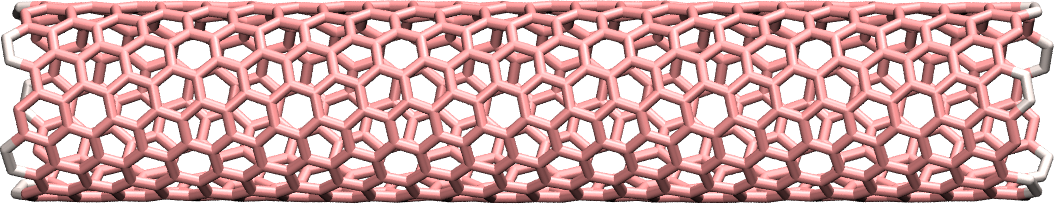
\includegraphics[width=\linewidth]{CNT-underformed}
\caption{CNT with the atoms from the \textit{carbon\_mid} group in pink,
and the atoms from the \textit{carbon\_top} and the \textit{carbon\_bot}
groups in white.}
\label{fig:CNT-underformed}
\end{figure}

Run the simulation using LAMMPS. The number of atoms in each group is given in
the \textit{Output} window. Always make sure that the number
of atoms in each group corresponds to what is expected, just like here:
{\normalsize \begin{verbatim}
10 atoms in group carbon_top
10 atoms in group carbon_bot
680 atoms in group carbon_mid
\end{verbatim}}
The atoms from the \textit{carbon\_top} and \textit{carbon\_bot} groups are
represented in white in Fig.\,\ref{fig:CNT-underformed}, and the atoms from
the \textit{carbon\_mid} group in pink.

Finally, to start from a less ideal state and create a system with some defects,
let us randomly delete a small fraction of the carbon atoms. To avoid deleting
atoms that are too close to the edges, let us define a new region name \textit{rdel}
that starts $2\,\text{\AA{}}$ from the CNT edges.
{\normalsize \begin{verbatim}
variable xmax_del equal ${xmax}-2
variable xmin_del equal ${xmin}+2
region rdel block ${xmin_del} ${xmax_del} &
    INF INF INF INF
group rdel region rdel
delete_atoms random fraction 0.02 no rdel &
    NULL 482793 bond yes
\end{verbatim}}
The \textit{delete\_atoms} command randomly deletes $2\,\%$ of the atoms from
the \textit{rdel} group (i.e. about 10 atoms) (Fig.\,\ref{fig:CNT-underformed-deleted}).

\begin{figure}
\centering
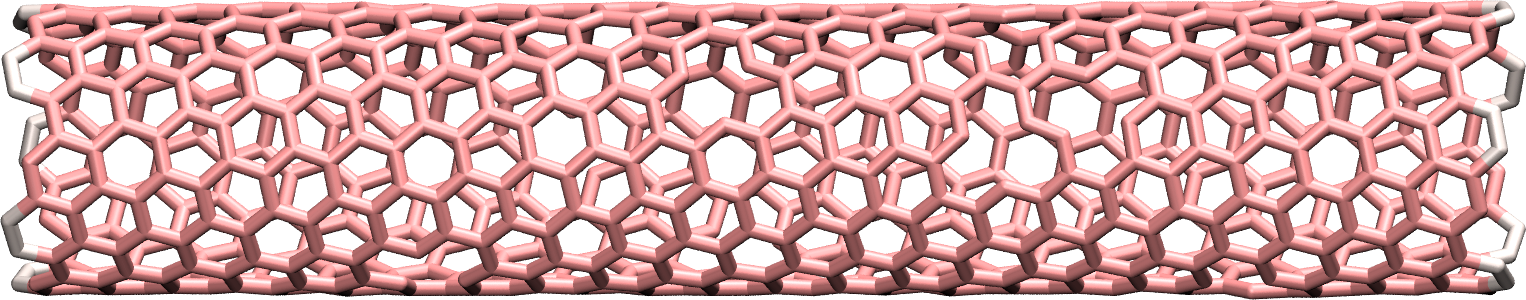
\includegraphics[width=\linewidth]{CNT-underformed-deleted}
\caption{Same CNT as in Fig.\,\ref{fig:CNT-underformed}, but with 10 deleted atoms.
The 10 deleted atoms were chosen randomly from the central part of the CNT.}
\label{fig:CNT-underformed-deleted}
\end{figure}

\paragraph{The molecular dynamics}

Let us give an initial temperature to the atoms of \textit{carbon\_mid}:
{\normalsize \begin{verbatim}
reset_atoms id sort yes
velocity carbon_mid create ${T} 48455 &
    mom yes rot yes
\end{verbatim}}
Re-setting the atom IDs is necessary before using the \textit{velocity} command
when atoms were deleted, which is done here with the \textit{reset\_atoms} command.
The \textit{velocity} command gives initial velocities to the atoms of the middle
group \textit{carbon\_mid}, ensuring an initial temperature of $300\,\text{K}$
for these atoms.

Let us specify the thermalization and the dynamics of the system. Add the following
lines into \textit{input.lmp}:
{\normalsize \begin{verbatim}
fix mynve all nve
compute Tmid carbon_mid temp
fix myber carbon_mid temp/berendsen &
    ${T} ${T} 100
fix_modify myber temp Tmid
\end{verbatim}}
 The \textit{fix nve}
is applied to all atoms so that all atom positions are recalculated at every step,
and a \textit{Berendsen} thermostat is applied to the atoms of the group
\textit{carbon\_mid} only \cite{berendsen1984molecular}. The
\textit{fix\_modify myber} ensures that the \textit{fix Berendsen} uses the
temperature of the group \textit{carbon\_mid} as an input, instead of the
temperature of the whole system. This is necessary to make sure that the frozen
edges won't bias the temperature. Note that the atoms of the edges do not need
a thermostat because their motion will be restrained, see below.

To restrain the motion of the atoms at the edges, let us add the following
commands to \textit{input.lmp}:
{\normalsize \begin{verbatim}
fix mysf1 carbon_top setforce 0 0 0
fix mysf2 carbon_bot setforce 0 0 0
velocity carbon_top set 0 0 0
velocity carbon_bot set 0 0 0
\end{verbatim}}
The two \textit{setforce} commands cancel the forces applied on the atoms of the
two edges, respectively. The cancellation of the forces is done at every step,
and along all 3 directions of space, $x$, $y$, and $z$, due to the use of
\textit{0 0 0}. The two \textit{velocity} commands set the initial velocities
along $x$, $y$, and $z$ to 0 for the atoms of \textit{carbon\_top} and
\textit{carbon\_bot}, respectively. As a consequence of these last four commands,
the atoms of the edges will remain immobile during the simulation (or at least
they would if no other command was applied to them).

On a side note, the \textit{velocity set}
commands impose the velocity of a group of atoms at the start of a run but do
not enforce the velocity during the entire simulation. When \textit{velocity set}
is used in combination with \textit{setforce 0 0 0}, as is the case here, the
atoms won't feel any force during the entire simulation. According to the Newton
equation, no force means no acceleration, meaning that the initial velocity
will persist during the entire simulation, thus producing a constant velocity motion.

\paragraph{Outputs}
Next, to measure the strain and stress applied to the CNT, let us create a
variable for the distance $L$ between the two edges, as well as  a variable $F$
for the force applied on the edges:
{\normalsize \begin{verbatim}
variable L equal &
    xcm(carbon_top,x)-xcm(carbon_bot,x)
variable F equal f_mysf1[1]-f_mysf2[1]
\end{verbatim}}
Here, the force is extracted from the fixes \textit{mysf1} and \textit{mysf2}
using \textit{f\_}, similarly to the use of \textit{v\_} to call a variable,
and \textit{c\_} to call a compute, as seen in \hyperref[lennard-jones-label]{Tutorial 1}.

Let us also add a \textit{dump image} command to visualize the system
every 500 steps:
{\normalsize \begin{verbatim}
dump mydmp all image 500 dump.*.jpg type type &
    shiny 0.1 box no 0.01 view 0 90 zoom 1.8
dump_modify mydmp acolor 1 pink &
    adiam 1 1 backcolor white
\end{verbatim}}
Let us run a small equilibration step to bring the system to the required
temperature before applying any deformation:
{\normalsize \begin{verbatim}
thermo 100
thermo_style custom step temp etotal v_L v_F
thermo_modify temp Tmid line yaml

timestep 1.0
run 5000
\end{verbatim}}
With the \textit{thermo\_modify} command, we specify to LAMMPS that the
temperature $T_\mathrm{mid}$ must be outputted, instead of the
temperature of the entire system. This choice is motivated by the presence of
frozen parts with an effective temperature of 0\,K, which makes the average
temperature of the entire system less relevant. The \textit{thermo\_modify}
command also imposes the use of the YAML format that can easily be read by
Python (see below).

Let us impose a constant velocity deformation on the CNT
by combining the \textit{velocity set} command with previously defined
\textit{fix setforce}. Add the following lines in the \textit{input.lmp} file,
right after the last \textit{run 5000} command:
{\normalsize \begin{verbatim}
velocity carbon_top set 0.0005 0 0
velocity carbon_bot set -0.0005 0 0
run 10000
\end{verbatim}}
The chosen velocity for the deformation is $100\,\text{m/s}$, or
$0.001\,\text{\AA{}/fs}$.

\begin{figure}
\centering
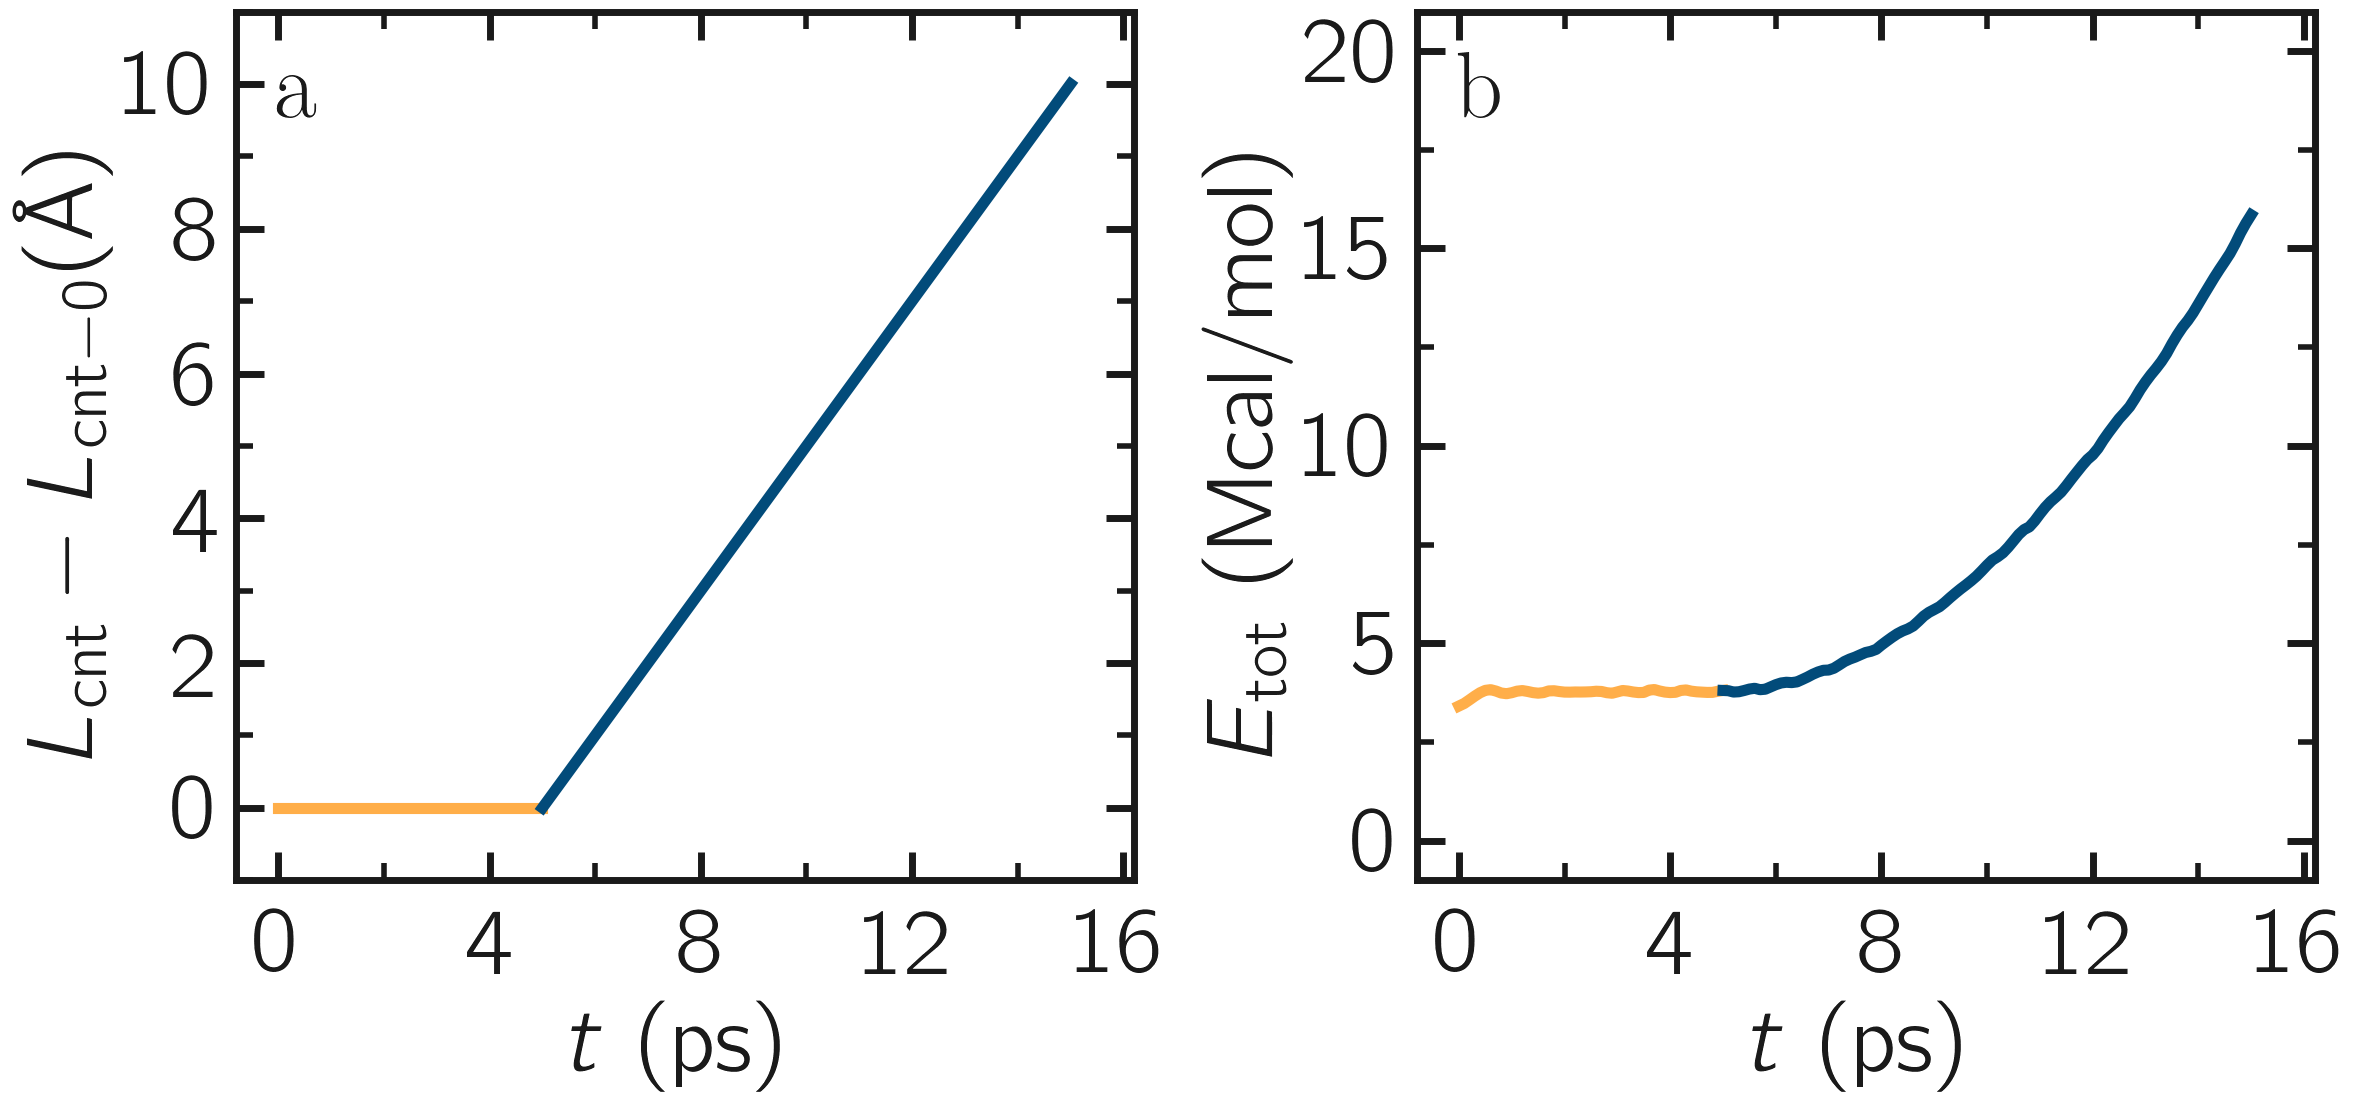
\includegraphics[width=\linewidth]{CNT-lenght-unbreakable}
\caption{Evolution of the length $L$ of the CNT with time. The CNT starts
deforming at $t = 5\,\text{ps}$.}
\label{fig:CNT-unbreakable-lenght}
\end{figure}

Run the simulation using LAMMPS. As can be seen from the variable $L$, the length
of the CNT increases linearly over time for $t > 5\,\text{ps}$ (Fig.\,\ref{fig:CNT-unbreakable-lenght}),
as expected from the imposed constant velocity. What you observe in the \textit{Slide Show}
windows should resembles Fig.\,\ref{fig:CNT-deformed-unbreakable}. The total energy of the system
shows a non-linear increase with $t$ once the deformation starts, which is expected
from the typical dependency of bond energy with bond distance,
$U_\text{b} = k_\text{b} \left( r - r_0 \right)^2$ (Fig.\,\ref{fig:CNT-unbreakable-energy}).

\begin{figure}
\centering
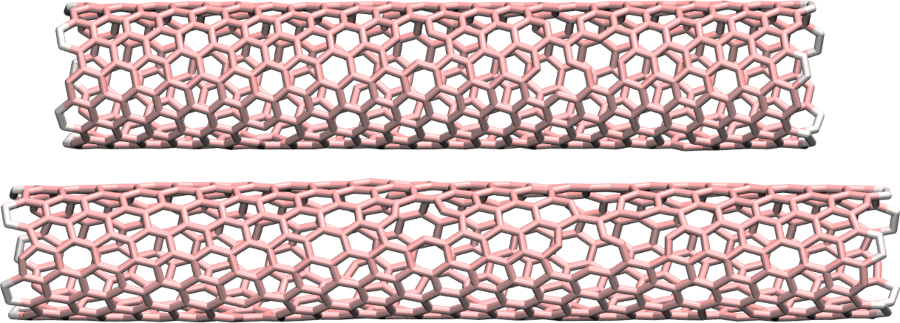
\includegraphics[width=\linewidth]{CNT-deformed-unbreakable}
\caption{CNT before (top) and after (bottom) deformation.}
\label{fig:CNT-deformed-unbreakable}
\end{figure}

\begin{figure}
\centering
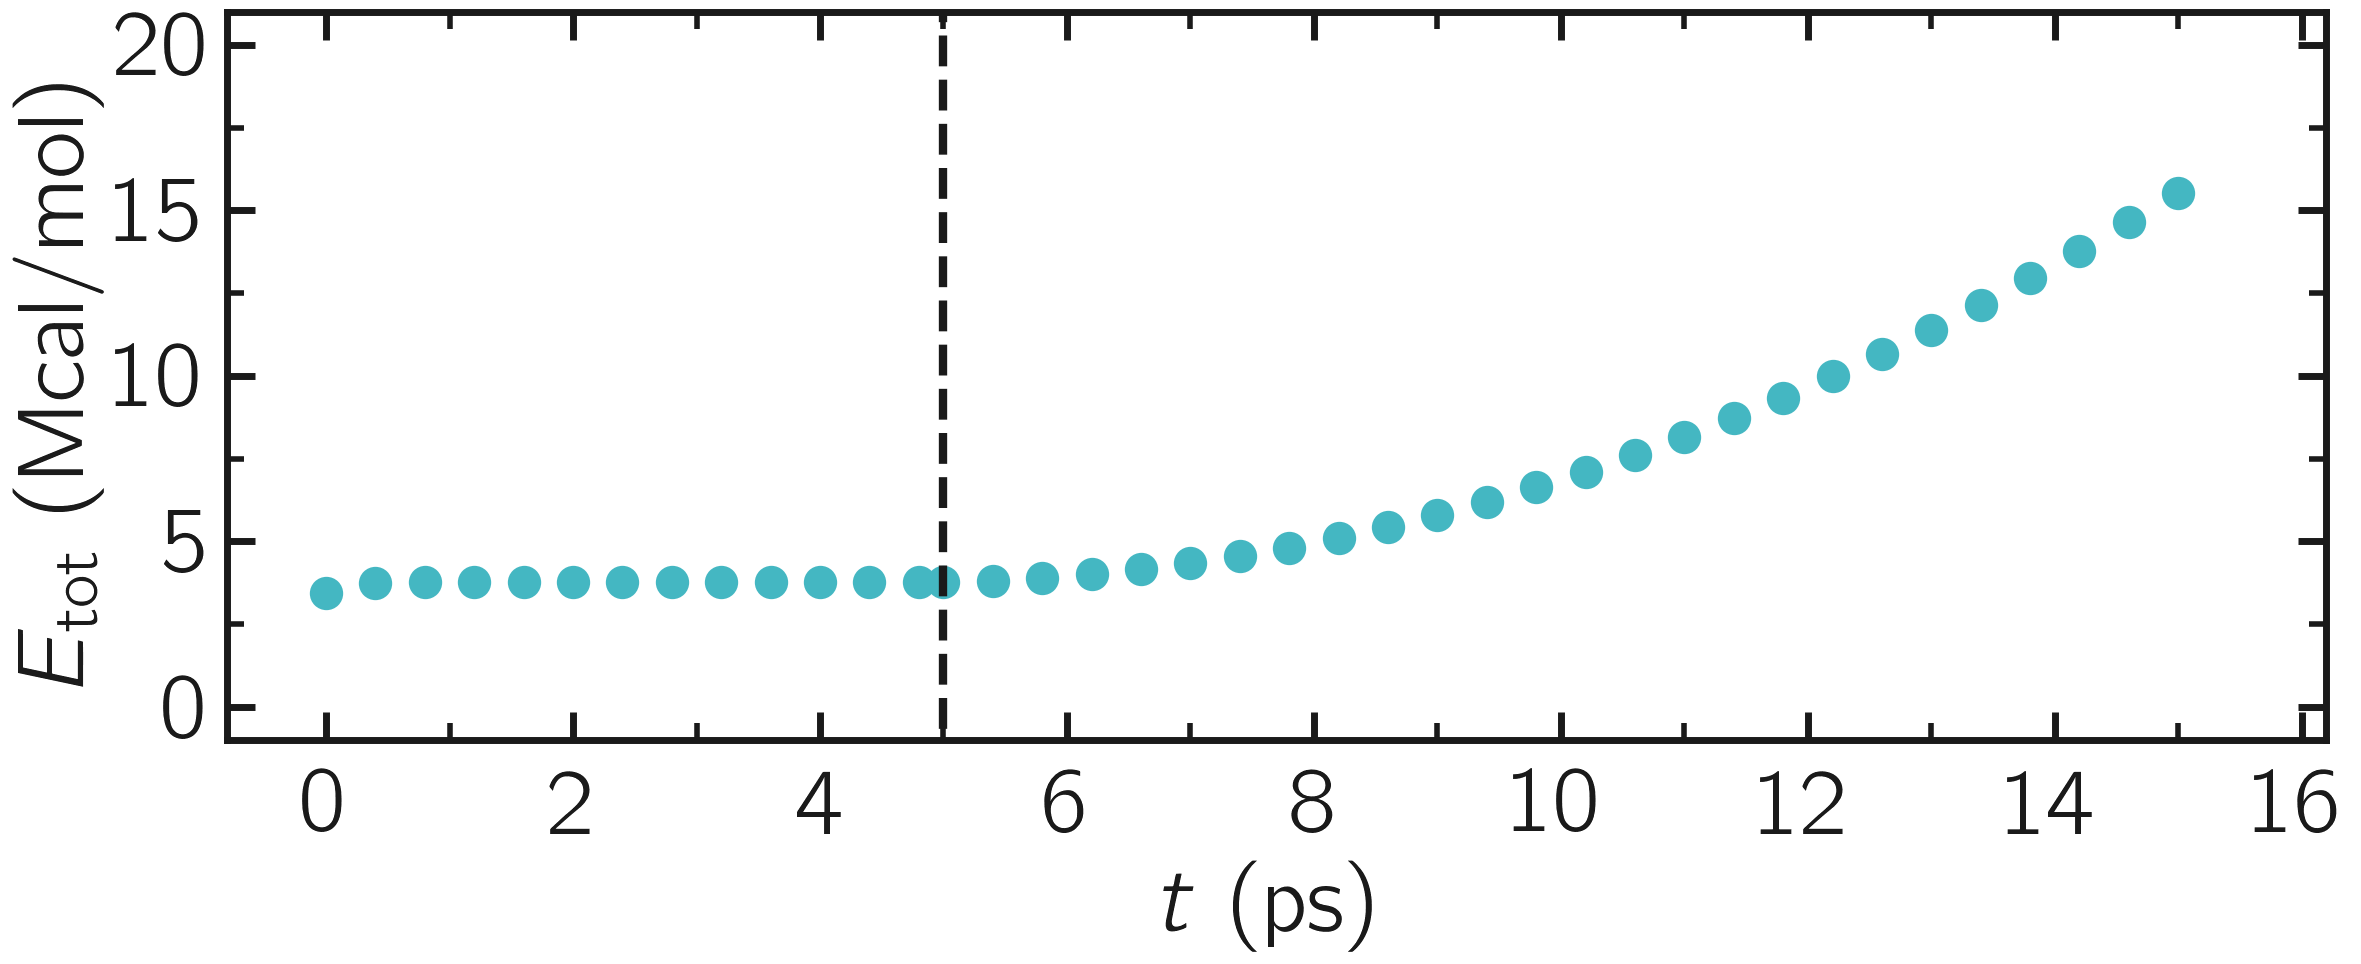
\includegraphics[width=\linewidth]{CNT-energy-unbreakable}
\caption{Evolution of the total energy $E_\text{tot}$ of the system with time $t$.
The CNT starts deforming at $t = 5\,\text{ps}$. The potential is OPLS-AA.}
\label{fig:CNT-unbreakable-energy}
\end{figure}

\paragraph{Importing YAML log file into Python}

Let us import the simulation data into Python, and generate the stress-strain curve.
Here, the stress is defined as $F/A$, where $A = \pi r^2$ is the surface area of the
CNT, and $r=5.2$\,\AA{} the CNT radius. The strain is defined as $(L-L_0)/L_0$,
where $L_0$ is the initial CNT length.

Right-click inside the \textit{Output} window, and select
\textit{Export YAML data to file}. Call the output \textit{log.yaml}, and save
it within \textit{unbreakable-bonds}. Download this script
\href{\filepath tutorial2/unbreakable-bonds/yaml-reader.py}{\textit{yaml-reader.py}} as well, and save it
within \textit{unbreakable-bonds/}. The \textit{yaml-reader.py} first imports
the \textit{log.yaml} file. Then, a certain pattern is
identified and stored as a string character named \textit{docs}. The string is
then converted into a list, and $F$ and $L$ are extracted. The stress and strain
are then calculated, and the result is saved in a data file using the
NumPy \textit{savetxt} function. \textit{thermo[0]} can be used to access the
information from the first minimization run, and \textit{thermo[1]} from
the second MD run. The data extracted from the \textit{log.yaml} file can
then be used to plot the stress-strain curve, see
Fig.\,\ref{fig:CNT-stress-strain-unbreakable}.

\begin{figure}
\centering
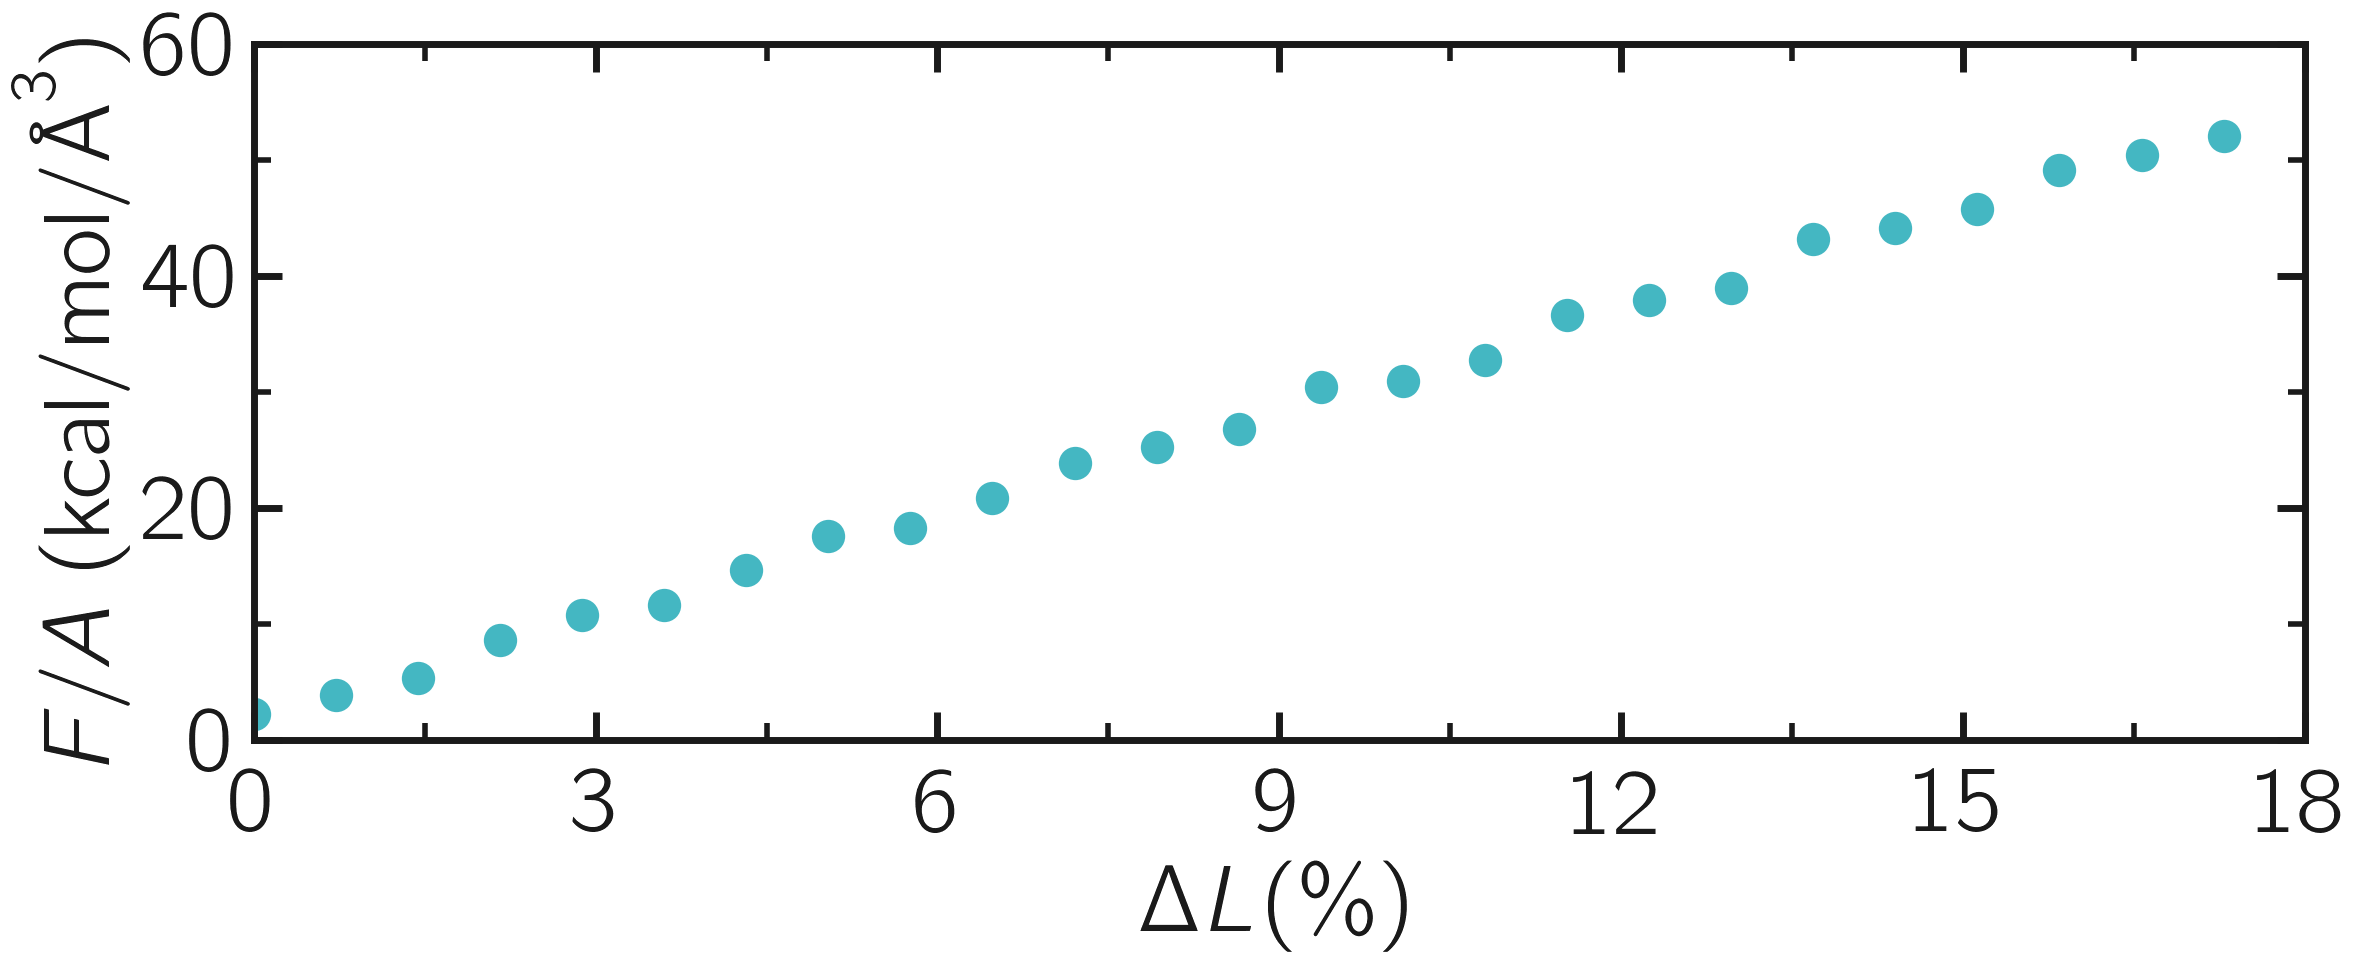
\includegraphics[width=\linewidth]{CNT-stress-strain-unbreakable}
\caption{Stress applied on the CNT during deformation $F/A$, where $F$ is the force
and $A$ the CNT surface area, as a function of the strain $(L-L_0/L_0)$, where
$L$ is the CNT length and $L_0$ the CNT initial length. The potential is OPLS-AA.}
\label{fig:CNT-stress-strain-unbreakable}
\end{figure}

\subsubsection{Breakable bonds}

When using a classical force field, as we just did, the bonds between the atoms
are non-breakable. Let us perform a similar simulation and deform a small
CNT again, but this time using a reactive force field that allows for the bonds
to break if the applied deformation is large enough.

\paragraph{Input file initialization}
Create a second folder called \textit{breakable-bonds/} next to
\textit{unbreakable-bonds/}, and create a new input file in it called
\textit{input.lmp}. Type into \textit{input.lmp}:
{\normalsize \begin{verbatim}
# Initialisation
variable T equal 300

units metal
atom_style atomic
boundary p p p
pair_style airebo 2.5 1 1
\end{verbatim}}
The first difference with the previous part is the unit system, here
\textit{metal} instead of \textit{real}, a choice that is imposed by the
AIREBO force field. A second difference is the use of the
\textit{atom\_style atomic} instead of \textit{molecular}, since no explicit
bond information is required with AIREBO.

\paragraph{Adapt the topology file}

Since \textit{bond}, \textit{angle}, and \textit{dihedral} do not need to be
explicitly set when using AIREBO, some simplification must be made to the
\textit{.data} file. Download the new \textit{.data}
file named \href{\filepath tutorial2/breakable-bonds/cnt_atom.data}{\textit{cnt\_atom.data}},
and place it within \textit{breakable-bonds/}. Just like \textit{cnt\_molecular.data},
the \textit{cnt\_atom.data} contains the information
required for placing the atoms in the box, but no bond/angle/dihedral information.
Another difference between \textit{cnt\_molecular.data} and \textit{cnt\_atom.data}
is that, here, a larger distance of 120 Ångstroms was used for the box size along
the \textit{x} axis, to allow for larger deformation.

\paragraph{Use of AIREBO potential}

Then, let us import the LAMMPS data file, and set the pair coefficients by adding
the following lines into \textit{input.lmp}:
{\normalsize \begin{verbatim}
# System definition
read_data cnt_atom.data
pair_coeff * * CH.airebo C
\end{verbatim}}
Here, there is one atom type, which we impose to be `carbon' by using
the letter \textit{C}. Download the \href{\filepath tutorial2/breakable-bonds/CH.airebo}{\textit{CH.airebo}}
file and place it within the \textit{breakable-bonds/} folder. The rest of the
\textit{input.lmp} is very similar to the previous one:

{\normalsize \begin{verbatim}
group carbon_atoms type 1

variable xmax equal &
    bound(carbon_atoms,xmax)-0.5
variable xmin equal &
    bound(carbon_atoms,xmin)+0.5
region rtop block ${xmax} INF INF INF INF INF
region rbot block INF ${xmin} INF INF INF INF
region rmid block &
    ${xmin} ${xmax} INF INF INF INF

group carbon_top region rtop
group carbon_bot region rbot
group carbon_mid region rmid

variable xmax_del equal ${xmax}-2
variable xmin_del equal ${xmin}+2
region rdel block ${xmin_del} ${xmax_del}&
    INF INF INF INF

group rdel region rdel
delete_atoms random fraction 0.02 no rdel &
    NULL 482793

reset_atoms id sort yes
velocity carbon_mid create ${T} 48455 &
    mom yes rot yes
fix mynve all nve
compute Tmid carbon_mid temp
fix myber carbon_mid temp/berendsen &
    ${T} ${T} 0.1
fix_modify myber temp Tmid
\end{verbatim}}

\paragraph{Start the simulation}
Here, let us impose a constant velocity deformation using the atoms of one
edge while maintaining the other edge fixed (note that for the unbreakable CNT,
the motion was imposed on the 2 edges). As an equilibration step, let us set the
velocity to 0 for the atoms of both edges. Add the following lines into
the \textit{input.lmp} file:
{\normalsize \begin{verbatim}
fix mysf1 carbon_bot setforce 0 0 0
fix mysf2 carbon_top setforce 0 0 0
velocity carbon_bot set 0 0 0
velocity carbon_top set 0 0 0

variable L equal &
    xcm(carbon_top,x)-xcm(carbon_bot,x)
variable F equal f_mysf1[1]-f_mysf2[1]

dump mydmp all image 5000 dump.*.jpg type type &
    shiny 0.1 box no 0.01 view 0 90 zoom 1.8
dump_modify mydmp acolor 1 pink &
    adiam 1 1 backcolor white

thermo 100
thermo_style custom step temp etotal v_L v_F
thermo_modify temp Tmid line yaml

timestep 0.0005
run 5000
\end{verbatim}}
Note the relatively small timestep of $0.0005\,\text{ps}$ used. A reactive force
field usually requires a smaller timestep than a classical one. When running
\textit{input.lmp} with LAMMPS, you can see that the temperature deviates
from the target temperature of $300\,\text{K}$ at the start of the equilibration,
but that after a few steps, it reaches the target value.

\paragraph{Launch the deformation}
After equilibration, let us set the velocity of one of the edges equal to
$15~\text{m/s}$ and run for a longer duration than previously. Add the following
lines into \textit{input.lmp}:
{\normalsize \begin{verbatim}
velocity carbon_top set 0.15 0 0
run 280000
\end{verbatim}}
Run the simulation. Some bonds are expected to break at approximately
two-thirds of the simulation (Fig.\,\ref{fig:CNT-deformed-breakable}).

\begin{figure}
\centering
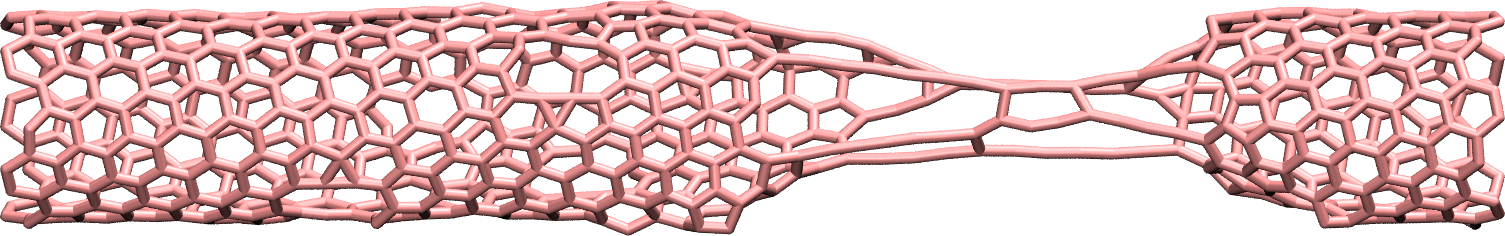
\includegraphics[width=\linewidth]{CNT-deformed-breakable}
\caption{CNT with broken bonds. Here, the \textit{DynamicBonds} representation
of VMD is used to properly visualize the bond breaking.}
\label{fig:CNT-deformed-breakable}
\end{figure}

Looking at the evolution of the energy, one can see that it is initially
increasing with the deformation. When bonds break, the energy relaxes abruptly,
as can be seen near $t=110~\text{ps}$ and again near $t=130~\text{ps}$ in
Fig.\,\ref{fig:CNT-breakable-energy}. Using the same script as previously to
import the data into Python, the stress-strain
curve can be generated, see Fig.\,\ref{fig:CNT-stress-strain-breakable}.

\begin{figure}
\centering
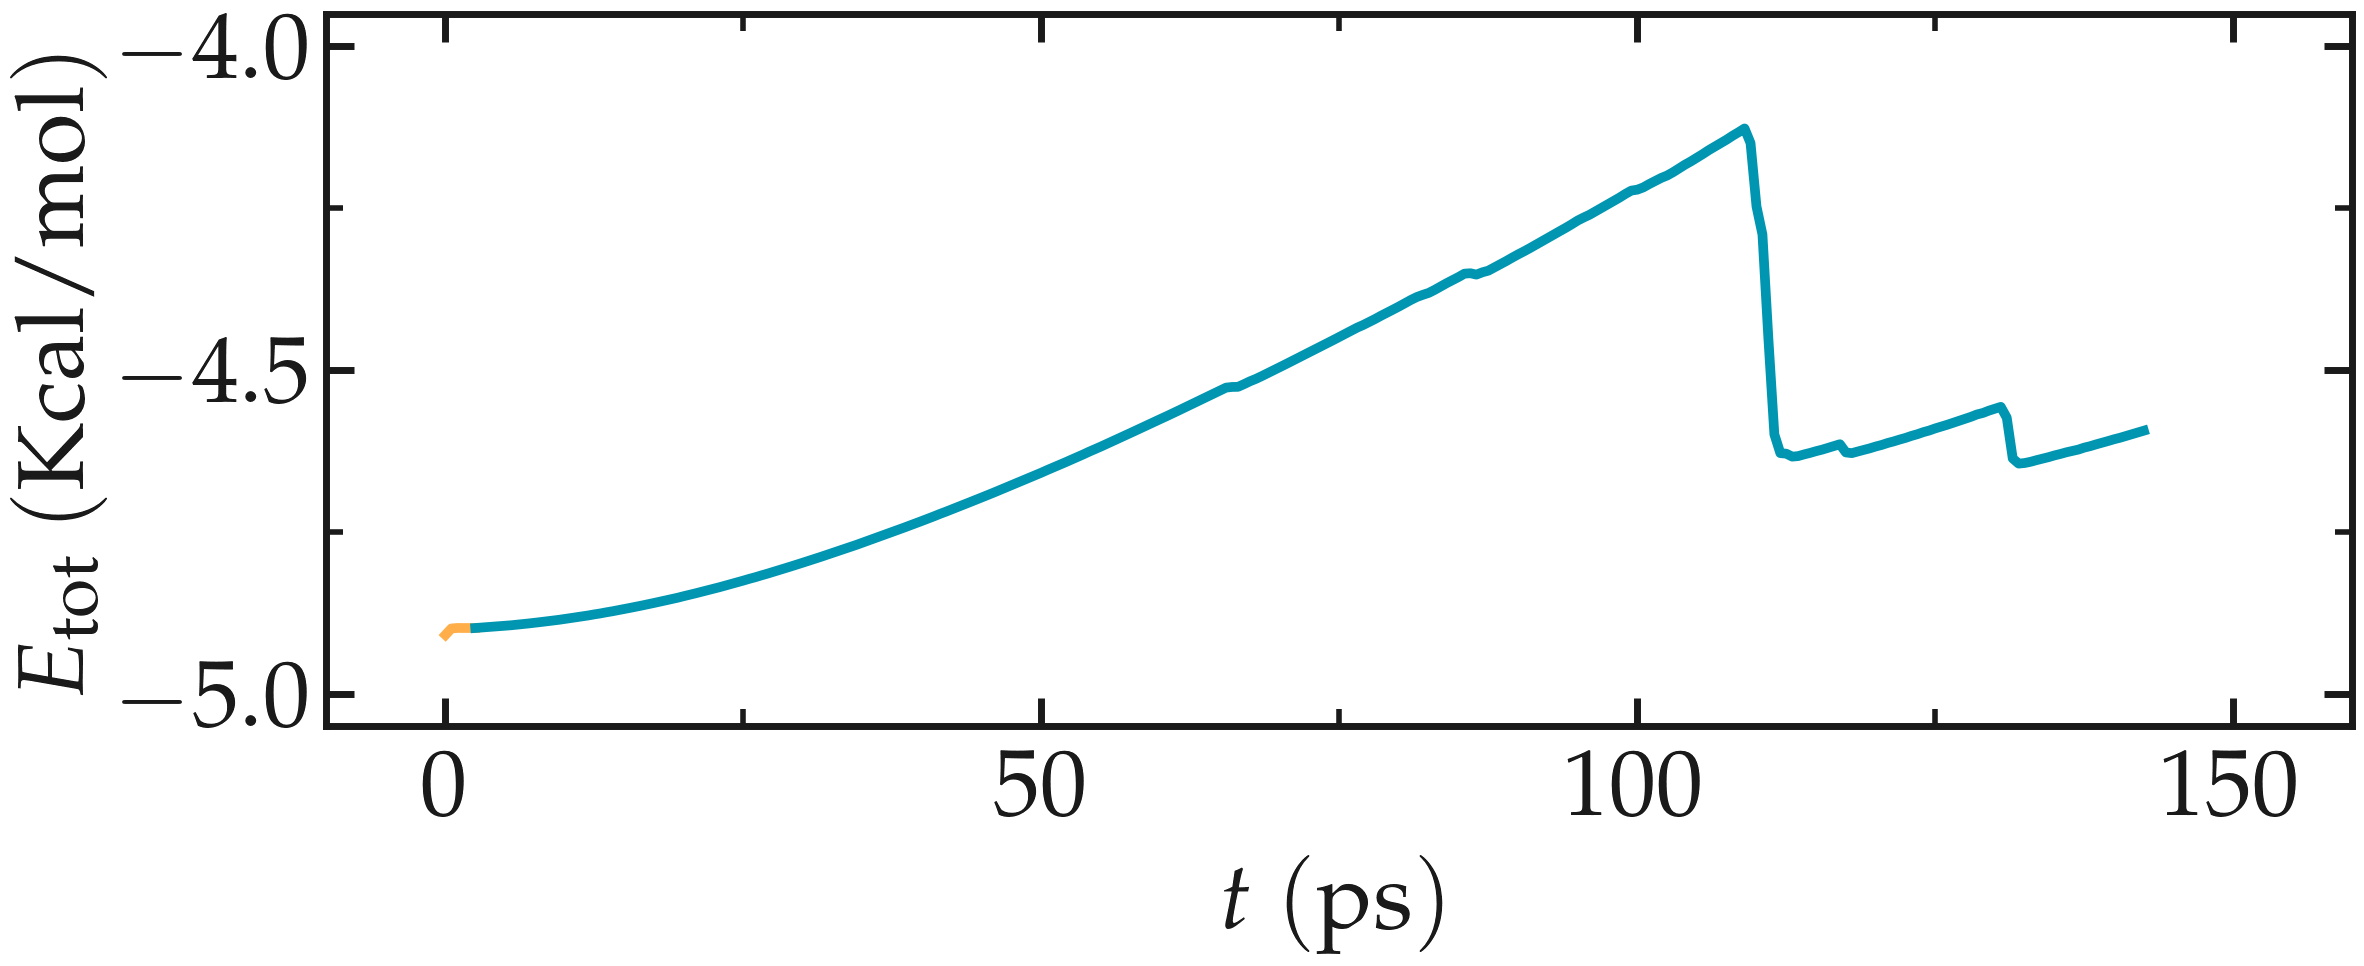
\includegraphics[width=\linewidth]{CNT-energy-breakable}
\caption{Evolution of the total energy $E_\text{tot}$ of the CNT with time $t$.
The potential is AIREBO.}
\label{fig:CNT-breakable-energy}
\end{figure}

\begin{figure}
    \centering
    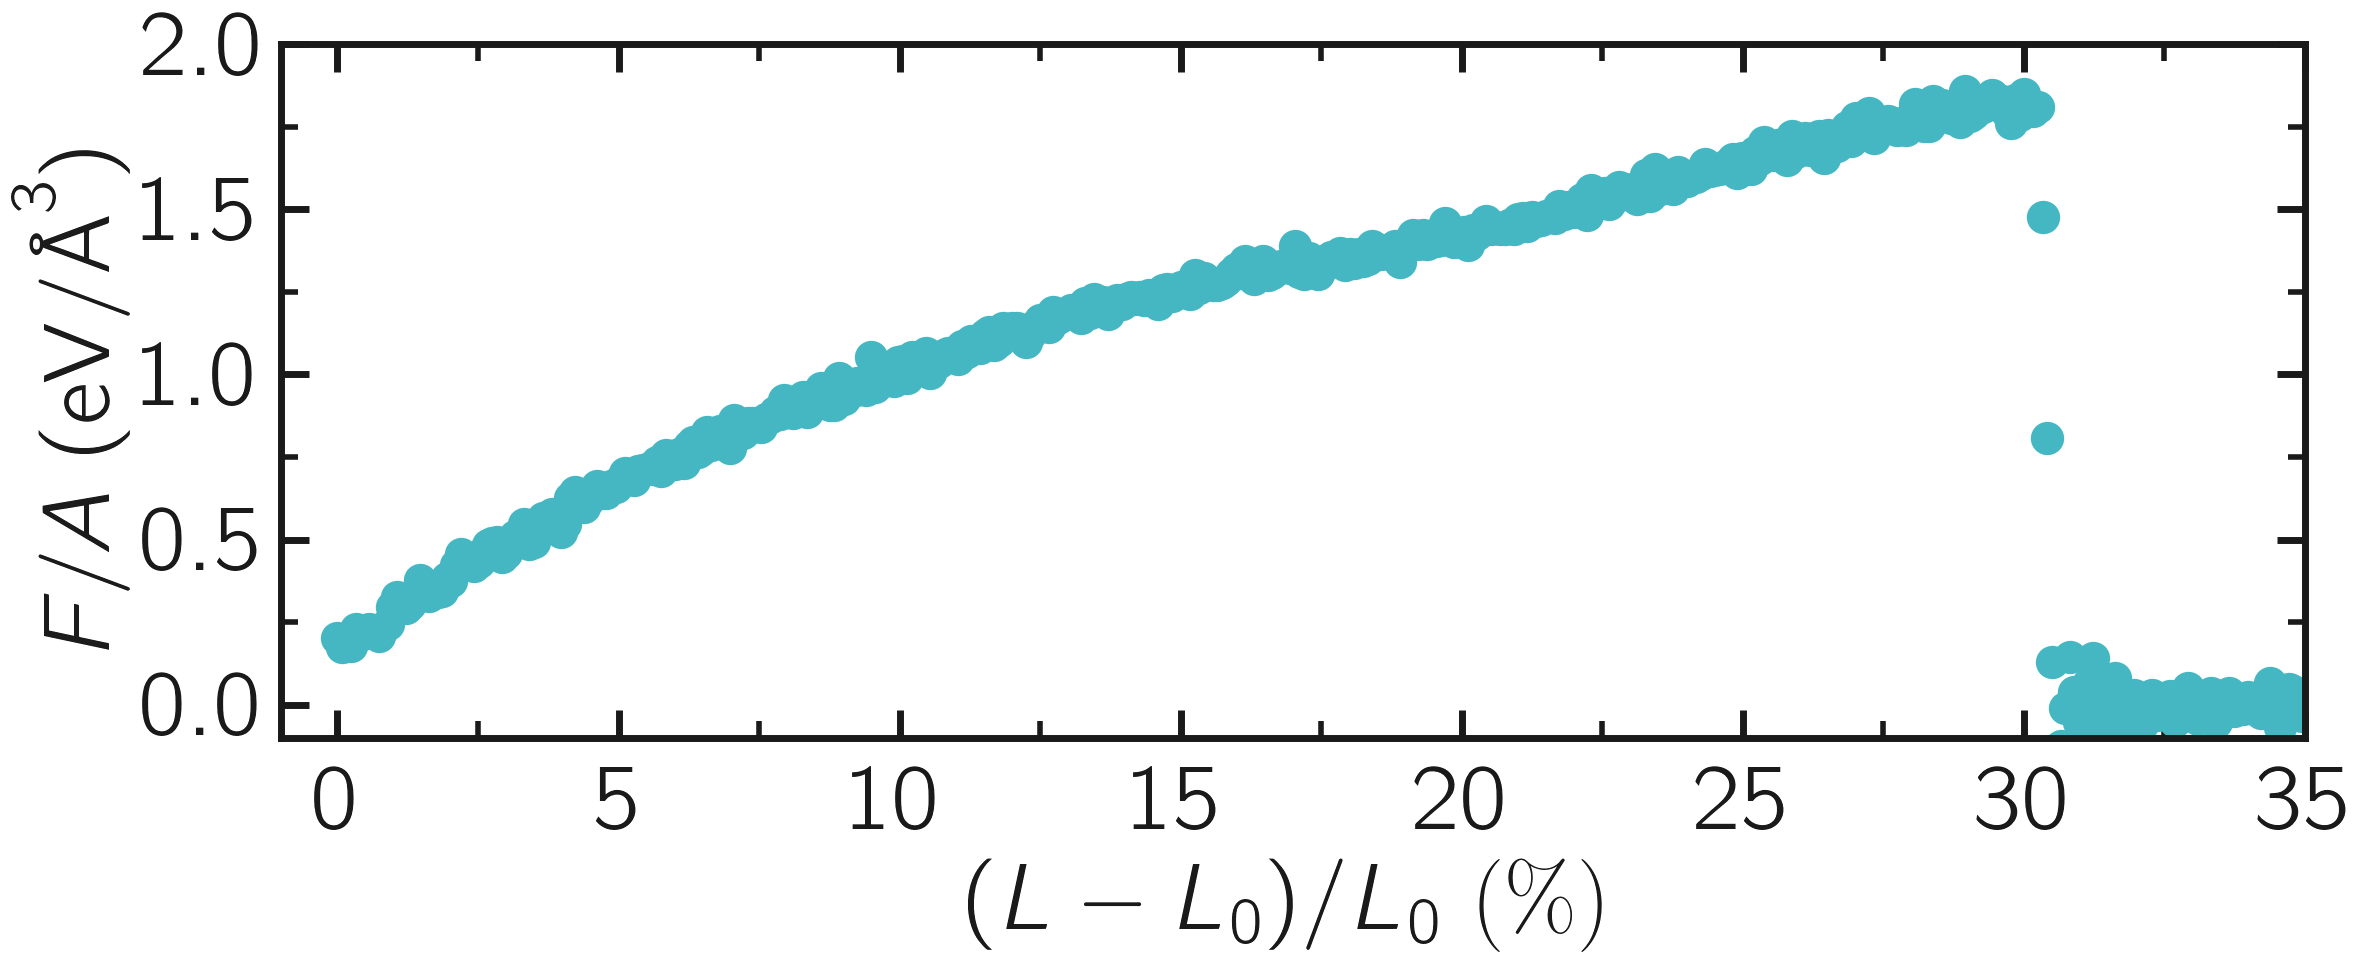
\includegraphics[width=\linewidth]{CNT-stress-strain-breakable}
    \caption{Stress applied on the CNT during deformation $F/A$, where $F$ is the force
    and $A$ the CNT surface area, as a function of the strain $(L-L_0/L_0)$, where
    $L$ is the CNT length and $L_0$ the CNT initial length. The potential is AIREBO.}
    \label{fig:CNT-stress-strain-breakable}
    \end{figure}

\subsection{Tutorial 3: Polymer in water}
\label{all-atoms-label}

\begin{figure}
\centering
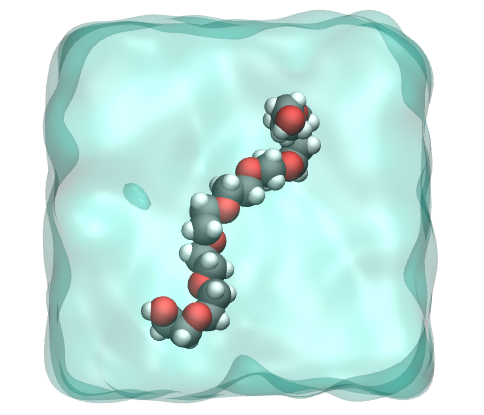
\includegraphics[width=0.55\linewidth]{PEG}
\caption{The polymer molecule (PEG - PolyEthylene Glycol) solvated in water as
simulated during \hyperref[all-atoms-label]{Tutorial 3}. Water molecules are
represented as a transparent continuum field for clarity.}
\label{fig:PEG}
\end{figure}

\noindent The goal of this tutorial is to use LAMMPS to solvate a small hydrophilic
polymer (PEG - PolyEthylene Glycol) in a reservoir of water (Fig.\,\ref{fig:PEG}).
Once the water reservoir is properly equilibrated at the desired temperature and
pressure, the polymer molecule is added and a constant stretching force is applied
to both ends of the polymer. The evolution of the polymer length is measured as
a function of time. The GROMOS 54A7 force field \cite{schmid2011definition} is used
for the PEG, the SPC/Fw model \cite{wu2006flexible} is used for the water, and the
long-range Coulomb interactions are solved using the PPPM solver \cite{luty1996calculating}.
This tutorial was inspired by a publication by Liese and coworkers, in which molecular
dynamics simulations are compared with force spectroscopy experiments \cite{liese2017hydration}.

\subsubsection{Preparing the water reservoir}

In this tutorial, the water reservoir is first prepared in the absence of the polymer.
A rectangular box of water is created and equilibrated at ambient temperature and
ambient pressure. The SPC/Fw water model is used \cite{wu2006flexible}, which is
a flexible variant of the rigid SPC (simple point charge) model \cite{berendsen1981interaction}.
Create a folder called \textit{pureH2O/}. Inside this folder, create an empty text
file called \textit{input.lmp}. Copy the following lines into it:
{\normalsize \begin{verbatim}
units real
atom_style full
bond_style harmonic
angle_style harmonic
dihedral_style harmonic
pair_style lj/cut/coul/long 10
kspace_style pppm 1e-5
special_bonds lj 0.0 0.0 0.5 &
    coul 0.0 0.0 1.0 angle yes
\end{verbatim}}
With the unit style \textit{real}, masses are in grams per mole, distances in
Ångstroms, time in femtoseconds, and energies in kcal/mole. With the \textit{atom\_style full}, each atom is a dot with a mass and a charge that can be linked by bonds, angles, dihedrals, and/or impropers. The \textit{bond\_style},
\textit{angle\_style}, and \textit{dihedral\_style} commands define the potentials
for the bonds, angles, and dihedrals used in the simulation, here \textit{harmonic}.
Finally, the \textit{special\_bonds} command, which was already seen in
\hyperref[carbon-nanotube-label]{tutorial 2}, sets the LJ and Coulomb weighting
factors for the interaction between neighboring atoms. With the \textit{pair\_style}
named \textit{lj/cut/coul/long}, atoms interact through both a Lennard-Jones (LJ)
potential and Coulomb interactions. The value of $10\,\text{\AA{}}$ is the cutoff.
Finally, the \textit{kspace} command defines the long-range solver for the Coulomb
interactions. The \textit{pppm} style refers to particle-particle particle-mesh \cite{luty1996calculating}.

Then, let us create a 3D simulation box of dimensions $9 \times 3 \times 3 \; \text{nm}^3$,
and make space for 8 atom types (2 for the water, 6 for the polymer), 7 bond types
(1 for the water, 6 for the polymer), 8 angle types (1 for the water, 7 for the polymer),
and 4 dihedral types (only for the polymer). Copy the following lines into \textit{input.lmp}:
{\normalsize \begin{verbatim}
region box block -45 45 -15 15 -15 15
create_box 8 box &
bond/types 7 &
angle/types 8 &
dihedral/types 4 &
extra/bond/per/atom 3 &
extra/angle/per/atom 6 &
extra/dihedral/per/atom 10 &
extra/special/per/atom 14
\end{verbatim}}
The \textit{extra/x/per/atom} commands are here for
memory allocation. We will use a file named \textit{PARM.lmp} that contains
all the parameters (masses, interaction energies, bond equilibrium
distances, etc). In \textit{input.lmp}, add the following line:
{\normalsize \begin{verbatim}
include ../PARM.lmp
\end{verbatim}}

Download and save the
\href{https://raw.githubusercontent.com/lammpstutorials/lammpstutorials-article/main/files/tutorial3/PARM.lmp}{\textit{PARM.lmp}}
file next to the \textit{pureH2O/} folder. This example uses type labels, which
are strings that map to each of the numeric atom types, bond types, angles types,
etc. in the simulation. Type labels can be any string defined by the user, and we
will use the atom types from the GROMOS 54A7 force field. In this example, the atom
types are defined in \textit{PARM.lmp}, within which the \textit{mass}
and \textit{pair\_coeff} of atoms of types OW and HW are for water and the remaining
atom types are for the polymer molecule. Similarly, the \textit{bond\_coeff HW-OW}
and \textit{angle\_coeff HW-OW-HW} are for water, while all the other parameters
are for the polymer.

Let us create water molecules. To do so, let us import a molecule template called
\textit{H2O-SPCFw.mol} and then randomly create 1050 molecules. Add the following
lines into \textit{input.lmp}:
{\normalsize \begin{verbatim}
molecule h2omol H2O-SPCFw.mol
create_atoms 0 random 1050 87910 NULL mol &
    h2omol 454756 overlap 1.0 maxtry 50
\end{verbatim}}
The \textit{overlap 1} option of the \textit{create\_atoms} command ensures
that no atoms are placed exactly in the same position, as this would cause the
simulation to crash. The \textit{maxtry 50} asks LAMMPS to try at most 50 times
to insert the molecules, which is useful in case some insertion attempts are
rejected due to overlap. In some cases, depending on the system and the values
of \textit{overlap} and \textit{maxtry}, LAMMPS may not create the desired number
of molecules. Always check the number of created atoms in the \textit{log} file
after starting the simulation:
{\normalsize \begin{verbatim}
Created 3150 atoms
\end{verbatim}}
When LAMMPS fails to create the desired number of molecules, a WARNING appears
in the \textit{log} file. The molecule template called
\href{https://raw.githubusercontent.com/lammpstutorials/lammpstutorials-article/main/files/tutorial3/H2O-SPCFw.mol}{\textit{H2O-SPCFw.mol}}
must be downloaded and saved in the \textit{pureH2O/} folder. This template contains
the necessary structural information of a water molecule, such as the number of
atoms, or the IDs of the atoms that are connected by bonds, angles, etc.

Then, let us organize the atoms of types OW and HW of the water molecules in a
group named \textit{H2O} and perform a small energy minimization. The energy
minimization is mandatory here given the small \textit{overlap} value of 1 Ångstrom
chosen in the \textit{create\_atoms} command. Add the following lines into \textit{input.lmp}:
{\normalsize \begin{verbatim}
group H2O type OW HW
minimize 1.0e-4 1.0e-6 100 1000
reset_timestep 0
\end{verbatim}}
In general, resetting the step of the simulation to 0 using the
\textit{reset\_timestep} command is optional.
It is used here because the number of iterations performed by the \textit{minimize}
command is usually not a round number (since the minimization stops when one of
four criteria is reached). Let us use the \textit{fix npt} to control the temperature
of the molecules with a Nosé-Hoover thermostat and the pressure of the system with
a Nosé-Hoover barostat \cite{nose1984unified, hoover1985canonical, martyna1994constant},
by adding the following line into \textit{input.lmp}:
{\normalsize \begin{verbatim}
fix mynpt all npt temp 300 300 100 &
    iso 1 1 1000
\end{verbatim}}
The \textit{fix npt} allows us to impose both a temperature of $300\,\text{K}$
(with a damping constant of $100\,\text{fs}$), and a pressure of 1 atmosphere
(with a damping constant of $1000\,\text{fs}$). With the \textit{iso} keyword,
the three dimensions of the box will be re-scaled simultaneously.

Let us print the atom positions in a \textit{.lammpstrj} file every 1000 steps
(i.e. 1 ps), print the temperature volume, and density every 100 steps in 3
separate data files, and print the information in the terminal every 1000 steps:
{\normalsize \begin{verbatim}
dump mydmp all atom 1000 dump.lammpstrj
variable mytemp equal temp
variable myvol equal vol
fix myat1 all ave/time 10 10 100 v_mytemp &
    file temperature.dat
fix myat2 all ave/time 10 10 100 v_myvol &
    file volume.dat
variable myoxy equal count(H2O)/3
variable mydensity equal ${myoxy}/v_myvol
fix myat3 all ave/time 10 10 100 v_mydensity &
    file density.dat
thermo 1000
\end{verbatim}}
The variable \textit{myoxy} corresponds to the number of atoms divided by 3, i.e.
the number of molecules.

Finally, let us set the timestep to 1.0 fs, and run the simulation for 20 ps by
adding the following lines into \textit{input.lmp}:
{\normalsize \begin{verbatim}
timestep 1.0
run 20000

write_data H2O.data
\end{verbatim}}
The final state is written into \textit{H2O.data}. If you open the \textit{dump.lammpstrj}
file using VMD, you should see the system quickly reaching its equilibrium volume
and density (see a snapshot of the equilibrated system in Fig.\,\ref{fig:PEG-water}).
You can also open the \textit{density.dat} file to ensure that the system converged
toward the density of liquid water during the 20 ps of simulation (Fig.\,\ref{fig:PEG-density}).

\begin{figure}
\centering
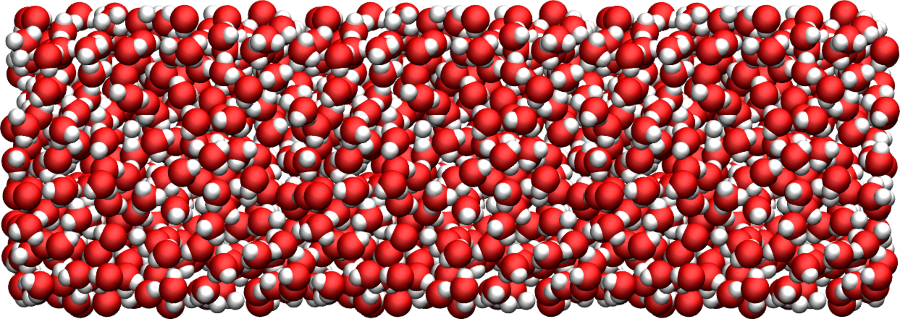
\includegraphics[width=\linewidth]{PEG-water}
\caption{Water reservoir after equilibration. Oxygen atoms are in red, and hydrogen
atoms are in white.}
\label{fig:PEG-water}
\end{figure}

\begin{figure}
\centering
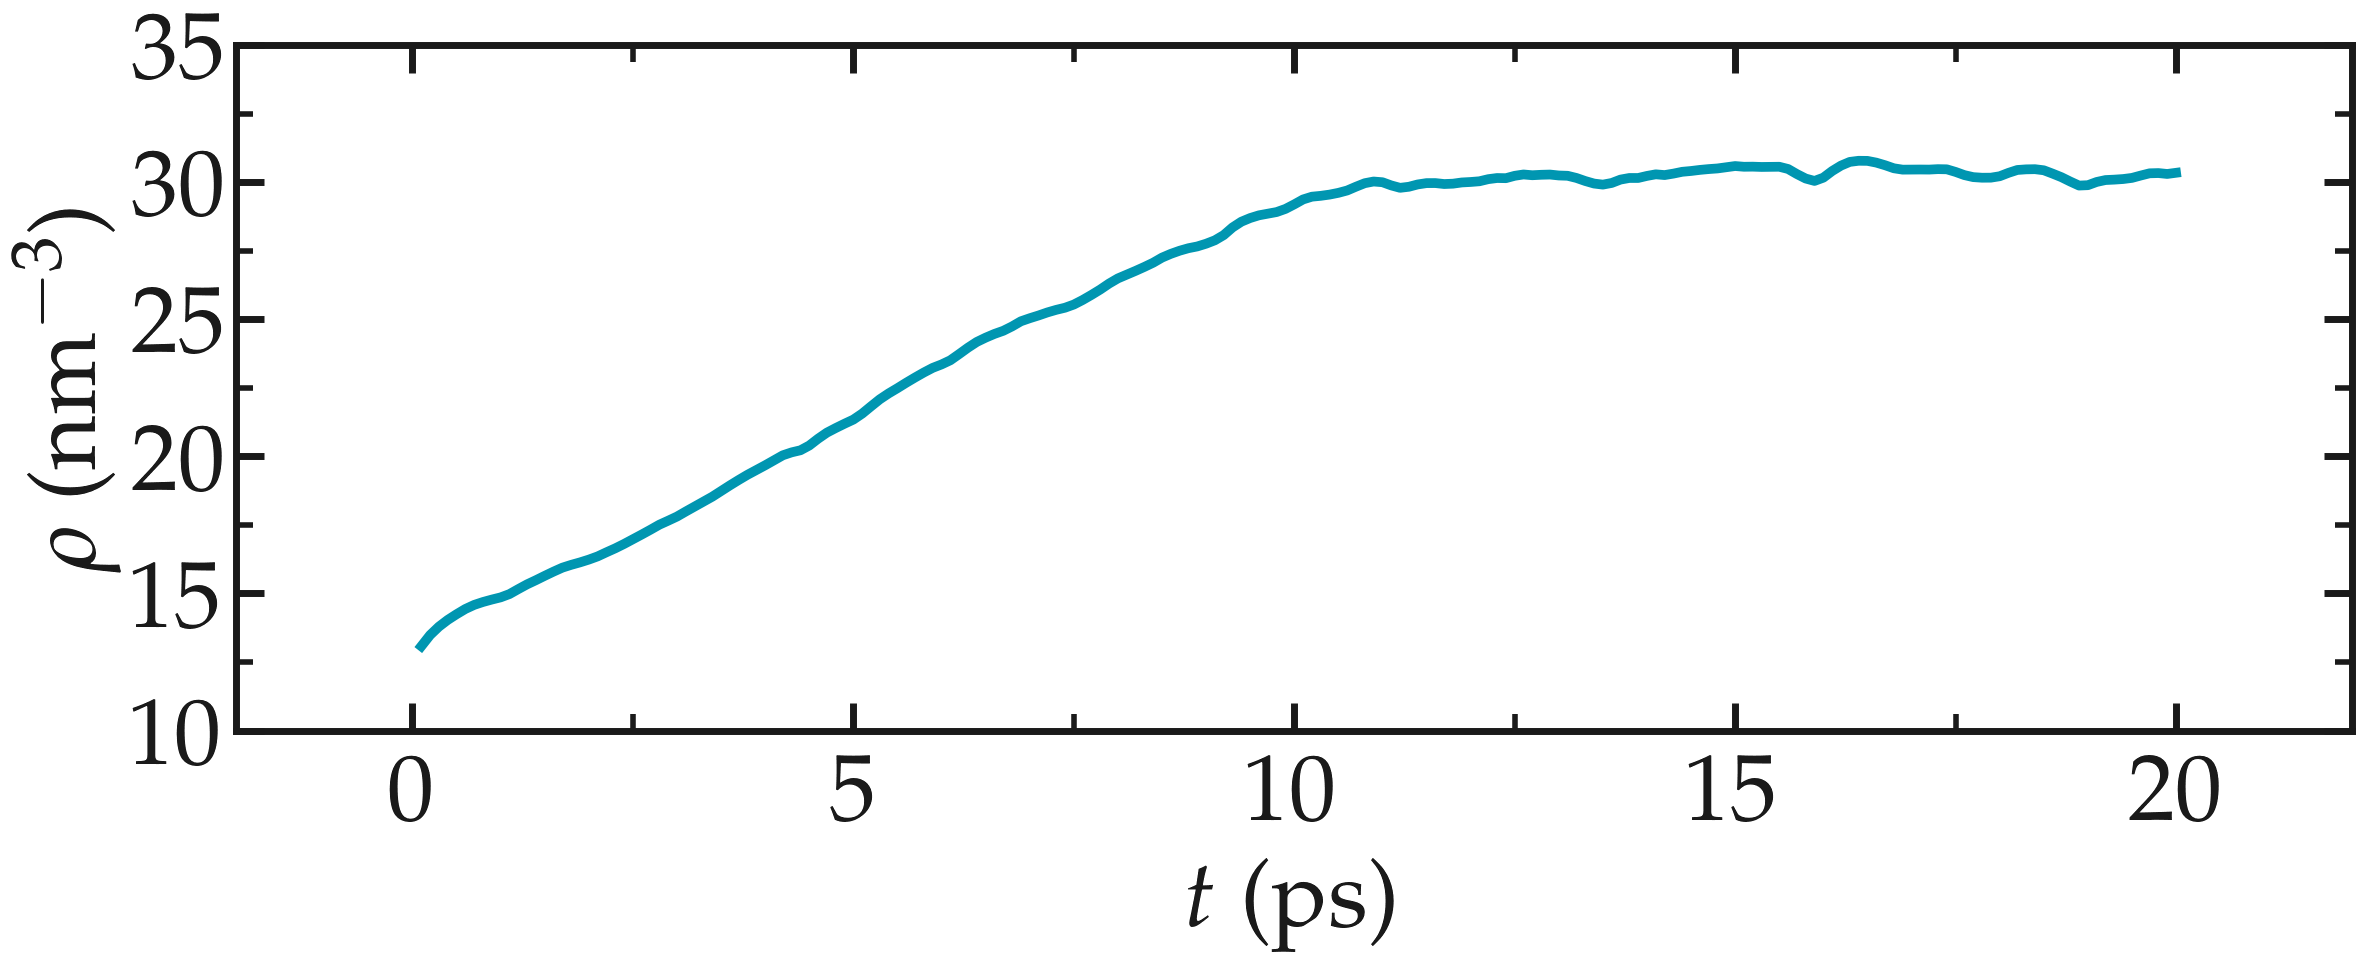
\includegraphics[width=\linewidth]{PEG-density}
\caption{Evolution of the density $\rho$ of water with time $t$. The density $\rho$
reaches a plateau after $t \approx 10\,\text{ps}$.}
\label{fig:PEG-density}
\end{figure}

\subsubsection{Solvating the PEG in water}
Now that the water reservoir is equilibrated, we can safely include the PEG polymer
in the water. The PEG molecule topology was downloaded from the ATB repository
\cite{malde2011automated, oostenbrink2004biomolecular}. It has a formula
$\text{C}_{28}\text{H}_{58}\text{O}_{15}$, and the parameters are taken from
the GROMOS 54A7 force field \cite{schmid2011definition}.

\begin{figure}
\centering
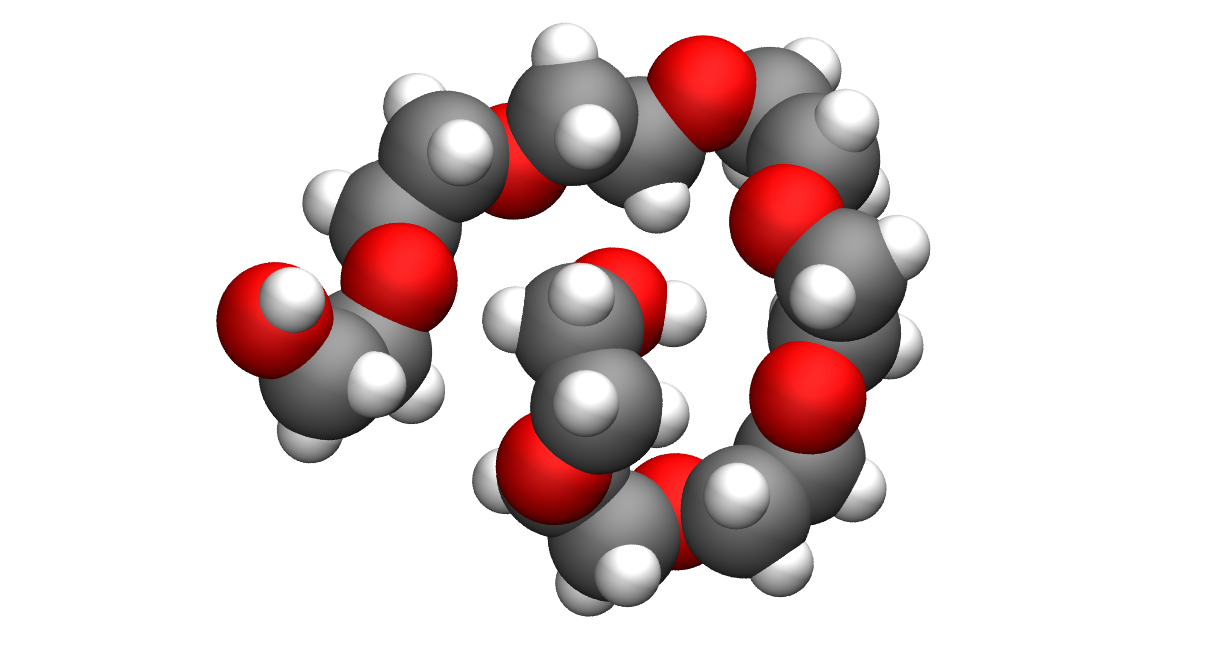
\includegraphics[width=\linewidth]{PEG-in-vacuum}
\caption{The PEG molecule in vacuum. The carbon atoms are in gray, the oxygen
atoms in red, and the hydrogen atoms in white.}
\label{fig:PEG-in-vacuum}
\end{figure}

Create a second folder alongside \textit{pureH2O/} and call it \textit{mergePEGH2O/}.
Create a new blank file in it, call it \textit{input.lmp}. Within \textit{input.lmp},
copy the same first lines as previously:
{\normalsize \begin{verbatim}
units real
atom_style full
bond_style harmonic
angle_style harmonic
dihedral_style harmonic
pair_style lj/cut/coul/long 10
kspace_style pppm 1e-5
special_bonds lj 0.0 0.0 0.5 coul 0.0 0.0 1.0 &
    angle yes dihedral yes
\end{verbatim}}
Then, import the previously generated data file \textit{H2O.data} as well as the \textit{PARM.lmp} file:
{\normalsize \begin{verbatim}
read_data ../pureH2O/H2O.data &
    extra/bond/per/atom 3 &
    extra/angle/per/atom 6 &
    extra/dihedral/per/atom 10 &
    extra/special/per/atom 14
include ../PARM.lmp
\end{verbatim}}
Download the template called
\href{https://raw.githubusercontent.com/lammpstutorials/lammpstutorials-article/main/files/tutorial3/PEG-GROMOS.mol}{\textit{PEG-GROMOS.mol}}
for the PEG molecule, and then create a single molecule in the middle of the box:
{\normalsize \begin{verbatim}
molecule pegmol PEG-GROMOS.mol
create_atoms 0 single 0 0 0 mol pegmol 454756
\end{verbatim}}
Let us create 2 groups to differentiate the PEG from the H2O, by adding the following
lines into \textit{input.lmp}:
{\normalsize \begin{verbatim}
group H2O type OW HW
group PEG type C CPos H HC OAlc OE
\end{verbatim}}
Water molecules that are overlapping with the PEG must be deleted to avoid future crashing.
Add the following line into \textit{input.lmp}:
{\normalsize \begin{verbatim}
delete_atoms overlap 2.0 H2O PEG mol yes
\end{verbatim}}
Here the value of 2 Ångstroms for the overlap cutoff was fixed arbitrarily and can
be chosen through trial and error. If the cutoff is too small, the simulation will
crash. If the cutoff is too large, too many water molecules will unnecessarily be
deleted. Finally, let us use the \textit{fix npt} to control the temperature, as
well as the pressure by allowing the box size to be rescaled along the \textit{x} axis:
{\normalsize \begin{verbatim}
fix mynpt all npt temp 300 300 100 x 1 1 1000
timestep 1.0
\end{verbatim}}
Once more, let us dump the atom positions as well as the system temperature and volume:
{\normalsize \begin{verbatim}
dump mydmp all atom 100 dump.lammpstrj
thermo 100
variable mytemp equal temp
variable myvol equal vol
fix myat1 all ave/time 10 10 100 &
    v_mytemp file temperature.dat
fix myat2 all ave/time 10 10 100 &
    v_myvol file volume.dat
\end{verbatim}}
Let us also print the total enthalpy:
{\normalsize \begin{verbatim}
variable myenthalpy equal enthalpy
fix myat3 all ave/time 10 10 100 &
    v_myenthalpy file enthalpy.dat
\end{verbatim}}
Finally, let us perform a short equilibration and print the
final state in a data file. Add the following lines to the data file:
{\normalsize \begin{verbatim}
run 30000
write_data mix.data
\end{verbatim}}
If you open the \textit{dump.lammpstrj} file using VMD or have a look at the
evolution of the volume in \textit{volume.dat}, you should see that the box
dimensions slightly evolve along \textit{x} to accommodate the new configuration.
In addition, the temperature remains close to the target value of $300~\text{K}$
throughout the entire simulation, and the enthalpy is almost constant, suggesting
that the system was close to equilibrium from the start.

\begin{figure}
\centering
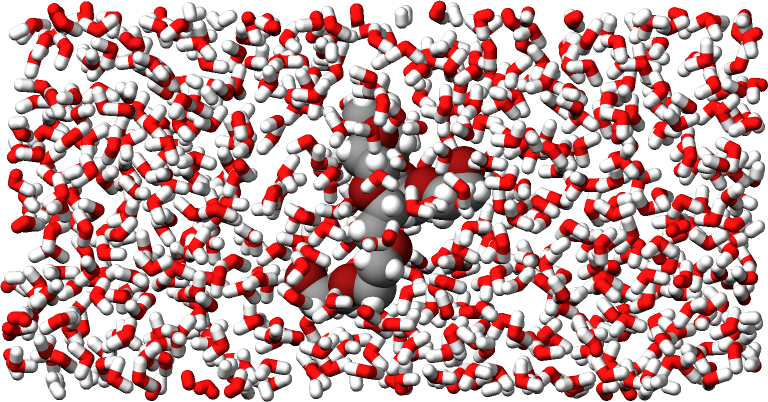
\includegraphics[width=\linewidth]{PEG-solvated}
\caption{A single PEG molecule in water. Water molecules are represented as a
transparent continuum field for clarity.}
\label{fig:PEG-solvated}
\end{figure}

\subsubsection{Stretching the PEG molecule}
Here, a constant forcing is applied to the two ends of the PEG molecule until it
stretches. Create a new folder next to the previously created folders, call it
\textit{pullonPEG/}, and create a new input file in it called \textit{input.lmp}.
First, let us create a variable \textit{f0} corresponding to the magnitude of the
force we are going to apply. Copy the following line into the \textit{input.lmp} file:
{\normalsize \begin{verbatim}
variable f0 equal 5
\end{verbatim}}
The force magnitude of $1\,\text{kcal/mol/\AA{}}$ corresponds to $67.2\,\text{pN}$
and was chosen to be large enough to overcome the thermal agitation and the entropic
contribution from both water and PEG molecules (it was chosen by trial and error).
Then, copy the same lines as previously:
{\normalsize \begin{verbatim}
units real
atom_style full
bond_style harmonic
angle_style harmonic
dihedral_style harmonic
pair_style lj/cut/coul/long 10
kspace_style pppm 1e-5
special_bonds lj 0.0 0.0 0.5 &
    coul 0.0 0.0 1.0 &
    angle yes dihedral yes
\end{verbatim}}
Start the simulation from the equilibrated PEG-water system and include again the
parameter file by adding the following lines to the \textit{input.lmp}:
{\normalsize \begin{verbatim}
read_data ../mergePEGH2O/mix.data
include ../PARM.lmp
\end{verbatim}}
Next, let us create some useful atom groups, including H2O and PEG (as previously),
as well as 2 groups containing a single atom each, the oxygen atoms at the ends
of the chain. Atoms of types OAlc correspond to the hydroxy (alcohol) group oxygen
atoms located at the ends of the PEG molecule, which we are going to use to pull
on the PEG molecule. Add the following lines to the \textit{input.lmp}:
{\normalsize \begin{verbatim}
group H2O type OW HW
group PEG type C CPos H HC OAlc OE
group ends type OAlc
variable xcm equal xcm(ends,x)
variable oxies atom type==label2type(atom,OAlc)
variable end1 atom v_oxies*(x>v_xcm)
variable end2 atom v_oxies*(x<v_xcm)
group topull1 variable end1
group topull2 variable end2
\end{verbatim}}
Add the following \textit{dump} command to the input to print the atom positions
every 1000 steps:
{\normalsize \begin{verbatim}
dump mydmp all atom 1000 dump.lammpstrj
\end{verbatim}}
Let us use a single Nosé-Hoover thermostat applied to all the atoms by adding the
following lines to \textit{input.lmp}:
{\normalsize \begin{verbatim}
timestep 1.0
fix mynvt all nvt temp 300 300 100
\end{verbatim}}
Let us also print the end-to-end distance of the PEG,
here defined as the distance between the groups \textit{topull1}
and \textit{topull2}, as well as the temperature of the system and the gyration
radius of the molecule \cite{fixmanRadiusGyrationPolymer1962a}
by adding the following lines to \textit{input.lmp}:
% S.G.: should we keep the data file, or just use thermo custom as its better for LAMMPS-GUI?
{\normalsize \begin{verbatim}
variable mytemp equal temp
fix myat1 all ave/time 10 10 100 &
    v_mytemp file temperature.dat
variable x1 equal xcm(topull1,x)
variable x2 equal xcm(topull2,x)
variable y1 equal xcm(topull1,y)
variable y2 equal xcm(topull2,y)
variable z1 equal xcm(topull1,z)
variable z2 equal xcm(topull2,z)
variable delta_r equal &
    sqrt((v_x1-v_x2)^2+(v_y1-v_y2)^2 &
    +(v_z1-v_z2)^2)
fix myat2 all ave/time 10 10 100 v_delta_r &
    file end-to-end-distance.dat
compute rgyr PEG gyration
fix myat3 all ave/time 10 10 100 c_rgyr &
    file gyration-radius.dat
thermo 1000
\end{verbatim}}
Finally, let us simulate 30 picoseconds without any external forcing:
{\normalsize \begin{verbatim}
run 30000
\end{verbatim}}
This first run will serve as a benchmark to quantify later the changes induced
by the forcing. Then, let us apply a forcing on the 2 oxygen atoms using two
\textit{add\_force} commands, and run for an extra 30 ps:
{\normalsize \begin{verbatim}
fix myaf1 topull1 addforce ${f0} 0 0
fix myaf2 topull2 addforce -${f0} 0 0
run 30000
\end{verbatim}}
Run the \textit{input.lmp} file using LAMMPS. If you open the \textit{dump.lammpstrj}
file using \textit{VMD}, you should see that the PEG molecule eventually aligns
in the direction of the force (as seen in Fig.\,\ref{fig:PEG-in-water}).
The evolutions of the end-to-end distance and of the gyration radius over
time show that the PEG is adjusting to the external forcing in less than
$10~\text{ps}$ (Fig.\,\ref{fig:PEG-distance}).

\begin{figure}
\centering
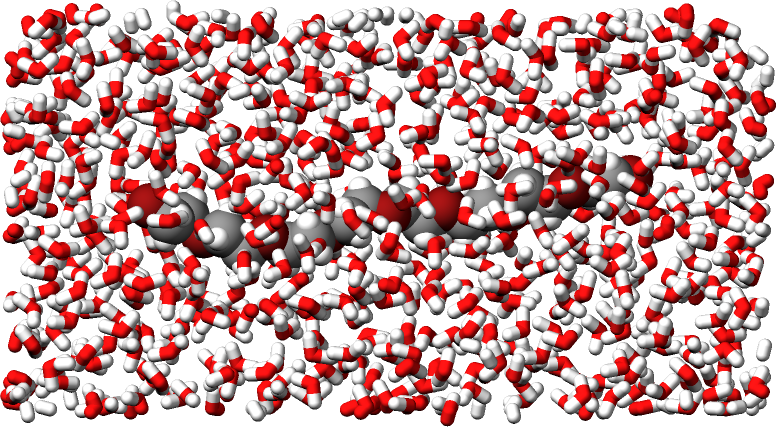
\includegraphics[width=\linewidth]{PEG-in-water}
\caption{PEG molecule stretched along the $x$ direction in water. Water molecules
are represented as a transparent continuum field for clarity.}
\label{fig:PEG-in-water}
\end{figure}

\begin{figure}
\centering
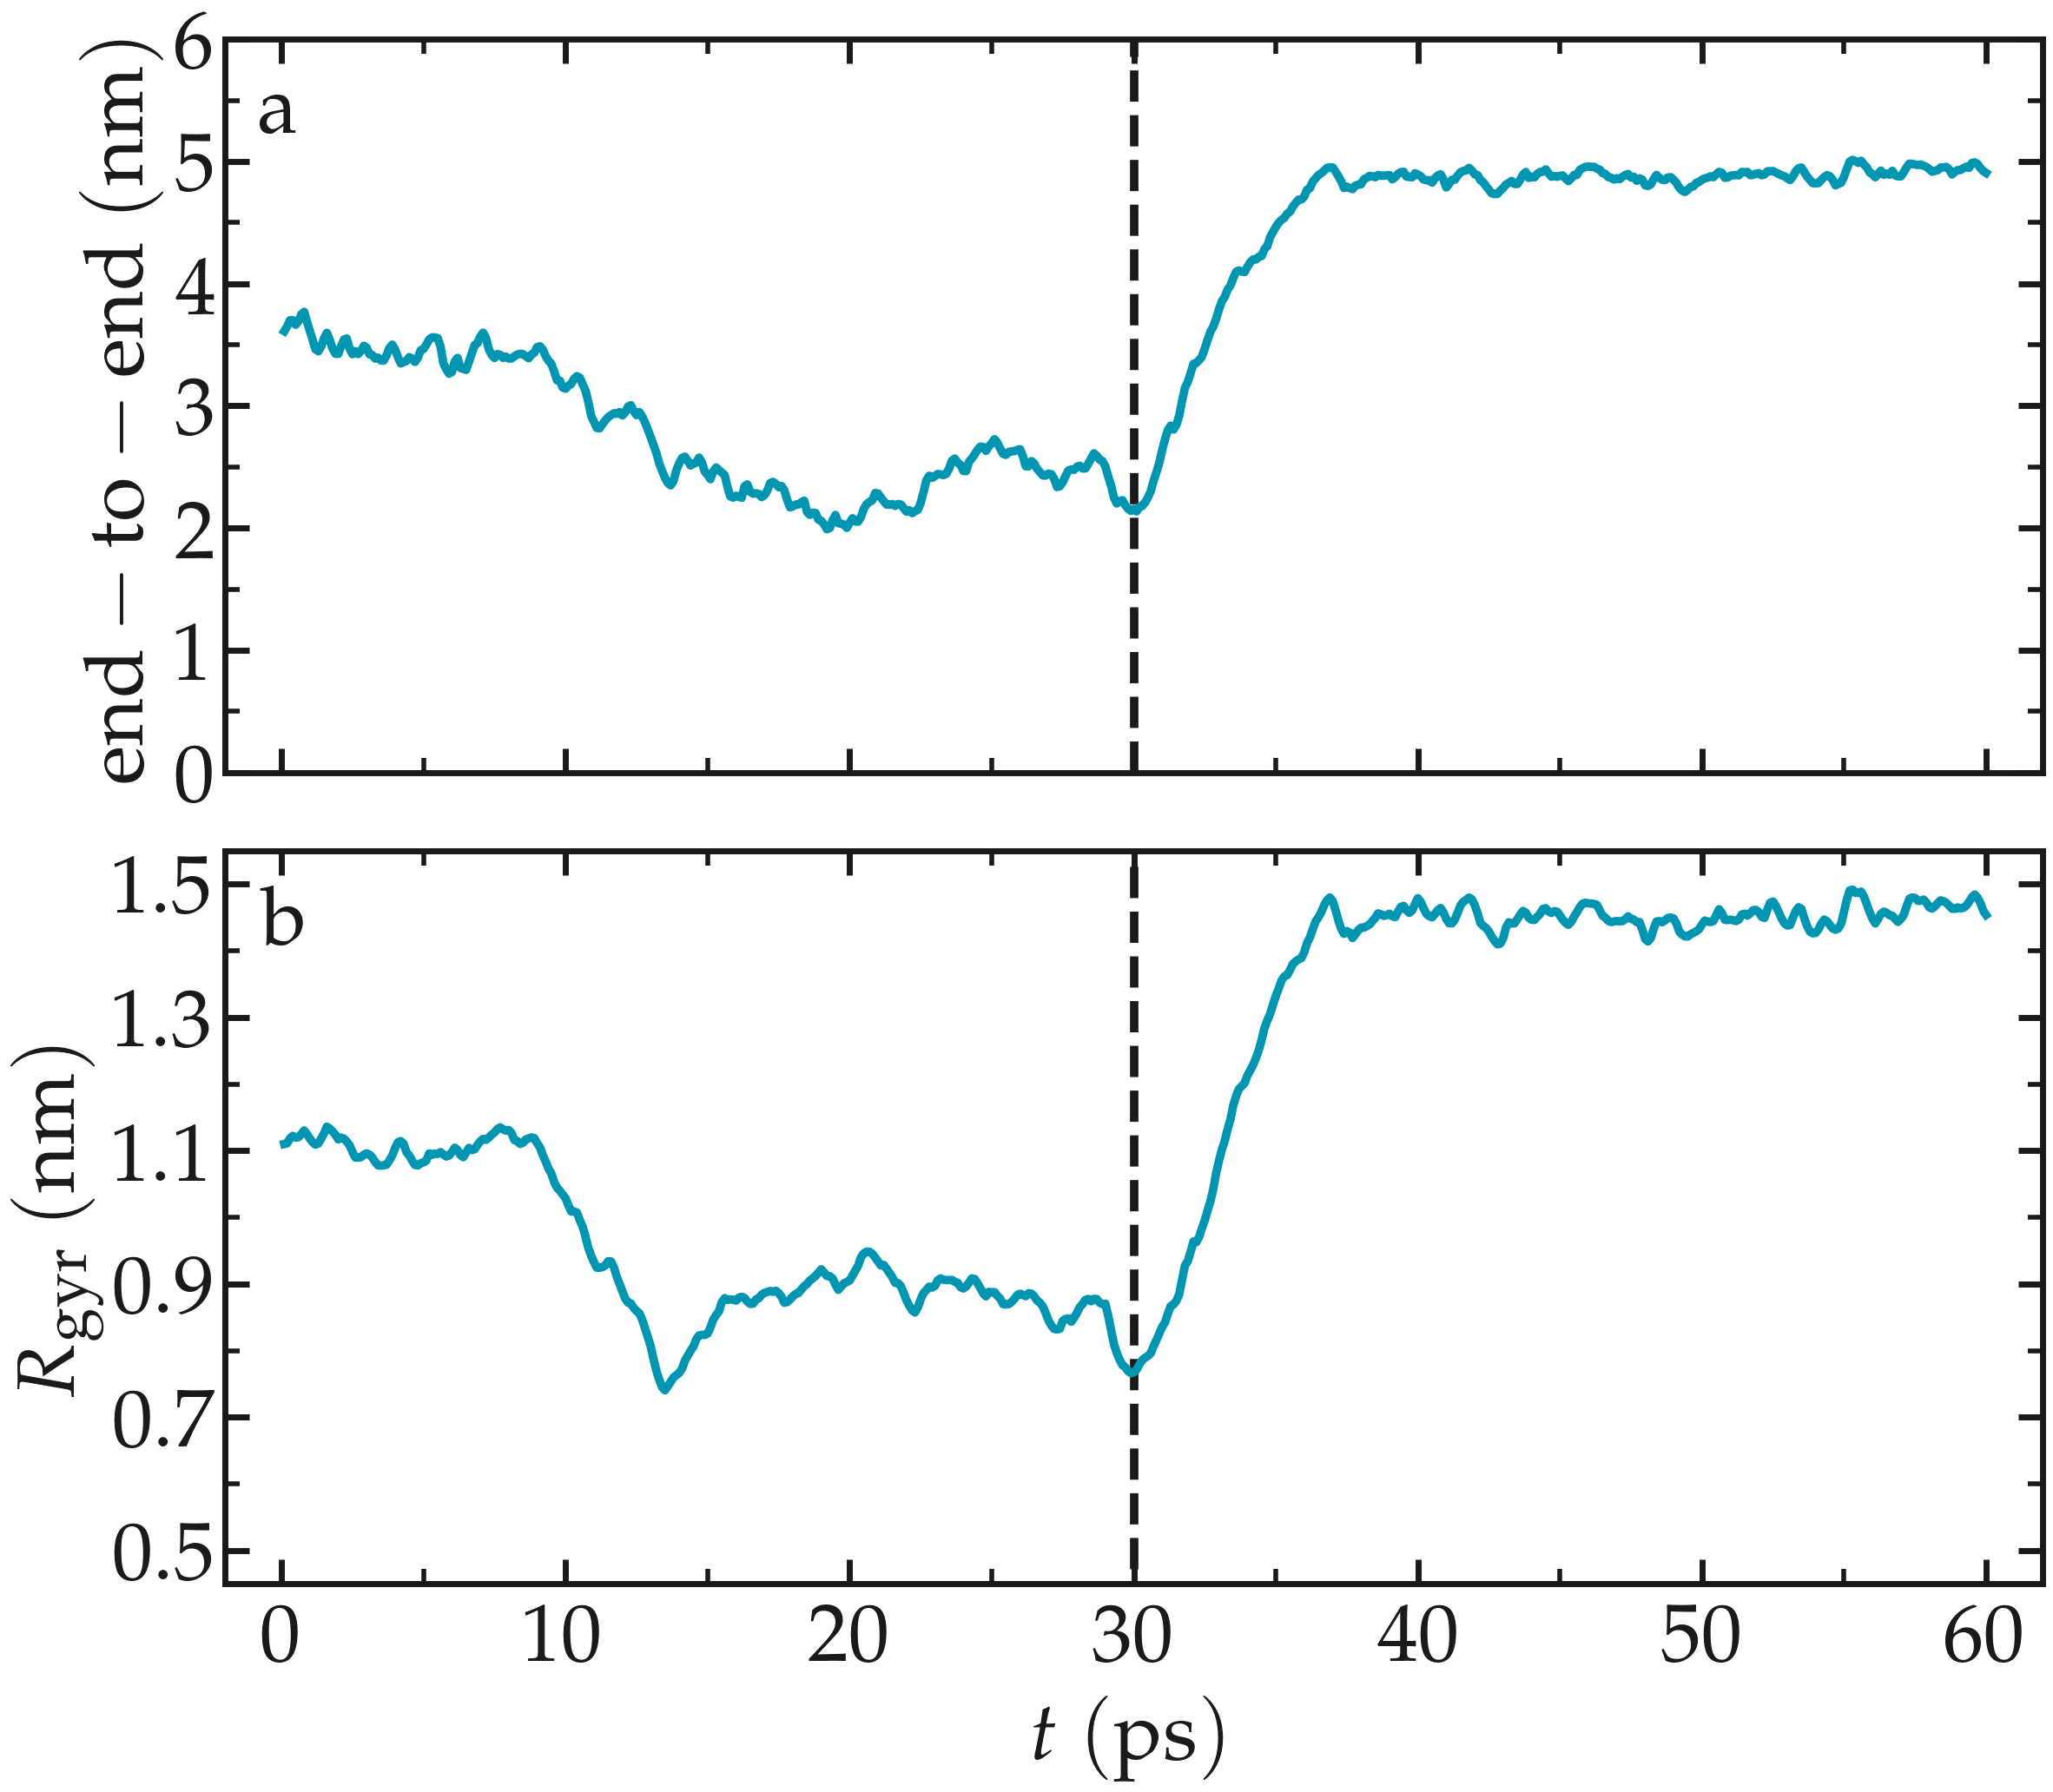
\includegraphics[width=\linewidth]{PEG-distance}
\caption{a) Evolution of the end-to-end distance $d_\text{end-to-end}$ of the
PEG with time $t$. The forcing starts at $t = 5\,\text{ps}$. b) Evolution of
the gyration radius $R_\text{gyr}$ of the PEG molecule.}
\label{fig:PEG-distance}
\end{figure}

\subsection{Tutorial 4: Nanosheared electrolyte}
\label{sheared-confined-label}

\begin{figure}
\centering
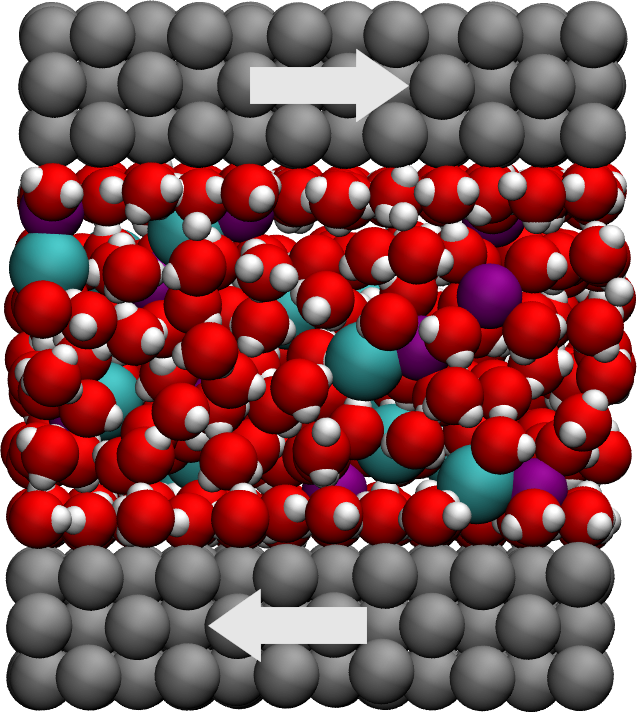
\includegraphics[width=0.55\linewidth]{NANOSHEAR}
\caption{The electrolyte confined in a nanometer slit pore as simulated during
\hyperref[sheared-confined-label]{Tutorial 4}. $\text{Na}^+$ ions are represented
as purple spheres, $\text{Cl}^-$ ions as cyan spheres, water molecules are colored
in red and white, and the walls are colored in gray. The arrows indicate the
imposed lateral motion of the walls.}
\label{fig:NANOSHEAR}
\end{figure}

\noindent The objective of this tutorial is to simulate an electrolyte
nanoconfined and sheared by two walls (Fig.\,\ref{fig:NANOSHEAR}). The density
and velocity profiles of the fluid in the direction normal to the walls are
extracted to highlight the effect of confining a fluid on its local properties.
This tutorial illustrates some key aspects of combining a fluid and a solid in
the same simulation. A major difference from the previous tutorial,
\hyperref[all-atoms-label]{Polymer in water}, is that here a rigid four-point
water model named TIP4P is used \cite{abascal2005general}. TIP4P is one of
the most common water models due to its high accuracy.

\subsubsection{System preparation}
The fluid and walls must first be generated and then equilibrated at a reasonable
temperature and pressure.

\paragraph{System generation}
Create a new folder called \textit{systemcreation/}. Within
\textit{systemcreation/}, open a blank file called \textit{input.lmp}, and
copy the following lines into it:
{\normalsize \begin{verbatim}
boundary p p f
units real
atom_style full
bond_style harmonic
angle_style harmonic
pair_style lj/cut/tip4p/long 1 2 1 1 &
    0.1546 12.0
kspace_style pppm/tip4p 1.0e-4
kspace_modify slab 3.0
\end{verbatim}}

These lines are used to define the most basic parameters, including the
\textit{atom}, \textit{bond}, and \textit{angle} styles, as well as interaction
potential. Here, \textit{lj/cut/tip4p/long} imposes a Lennard-Jones potential with
a cut-off at $12\,\text{$\text{\AA{}}$}$ and a long-range Coulomb potential.

So far, the commands are relatively similar to those in the previous tutorial,
\hyperref[all-atoms-label]{Polymer in water}, with two major differences: the use
of \textit{lj/cut/tip4p/long} instead of \textit{lj/cut/coul/long}, and \textit{pppm/tip4p}
instead of \textit{pppm}. When using \textit{lj/cut/tip4p/long} and \textit{pppm/tip4p},
the interactions resemble the conventional Lennard-Jones and Coulomb interactions,
except that they are specifically designed for the four-point water model. Therefore,
LAMMPS automatically creates a four-point water molecule using atoms of type O as
oxygen and atoms of type H as hydrogen. The fourth massless atom (\textit{M}) of the
TIP4P water molecule does not have to be defined explicitly, and the value of
$0.1546\,\text{$\text{\AA{}}$}$ corresponds to the \textit{O-M} distance of the
TIP4P-2005 water model \cite{abascal2005general}. All the other atoms in the simulation
are treated normally with long-range Coulomb interactions. Another novelty, here, is
the use of \textit{kspace\_modify slab 3.0} that is combined with the non-periodic
boundaries along the $z$ coordinate: \textit{boundary p p f}. With the \textit{slab}
option, the system is treated as periodical along $z$, but with an empty volume inserted
between the periodic images of the slab, and the interactions along $z$ effectively turned off.

Let us create the box by adding the following lines to \textit{input.lmp}:

{\normalsize \begin{verbatim}
lattice fcc 4.04
region box block -3 3 -3 3 -5 5
create_box 5 box &
bond/types 1 &
angle/types 1 &
extra/bond/per/atom 2 &
extra/angle/per/atom 1 &
extra/special/per/atom 2
\end{verbatim}}
The \textit{lattice} command defines the unit cell. Here, the face-centered cubic (fcc) lattice
with a scale factor of 4.04 has been chosen for the future positioning of the atoms
of the walls. The \textit{region} command defines a geometric region of space. By choosing
\textit{xlo=-3} and \textit{xhi=3}, and because we have previously chosen a lattice with a scale
factor of 4.04, the region box extends from $-12.12~\text{\AA{}}$ to $12.12~\text{\AA{}}$
along the $x$ direction. The \textit{create\_box} command creates a simulation box with
5 types of atoms: the oxygen and hydrogen of the water molecules, the two ions ($\text{Na}^+$,
$\text{Cl}^-$), and the atom of the walls. The \textit{create\_box} command extends over 6
lines thanks to the $\&$ character. The second and third lines are used to indicate that the
simulation contains 1 type of bond and 1 type of angle (both required by the water molecule).
The parameters for these bond and angle constraints will be given later. The three last
lines are for memory allocation.

Now, we can add atoms to the system. First, let us create two sub-regions corresponding
respectively to the two solid walls, and create a larger region from the union of the
two regions. Then, let us create atoms of type WALL within the two regions. Add the
following lines to \textit{input.lmp}:
{\normalsize \begin{verbatim}
region rbotwall block -3 3 -3 3 -4 -3
region rtopwall block -3 3 -3 3 3 4
region rwall union 2 rbotwall rtopwall
create_atoms WALL region rwall
\end{verbatim}}
Atoms will be placed in the positions of the previously defined lattice, thus
forming fcc solids. To add the water molecules, first download the molecule
template called \href{https://raw.githubusercontent.com/lammpstutorials/lammpstutorials-article/main/files/tutorial4/RigidH2O.txt}{\textit{RigidH2O.txt}}
and place it within \textit{systemcreation/}. The template contains all the
necessary information concerning the water molecule, such as atom positions,
bonds, and angles. Add the following lines to \textit{input.lmp}:
{\normalsize \begin{verbatim}
region rliquid block INF INF INF INF -2 2
molecule h2omol RigidH2O.txt
create_atoms 0 region rliquid mol h2omol 482793
\end{verbatim}}
Within the last three lines, a \textit{region} named \textit{rliquid} is
created based on the last defined lattice, \textit{fcc 4.04}. \textit{rliquid}
will be used for depositing the water molecules. The \textit{molecule} command
opens up the molecule template called \textit{RigidH2O.txt}, and names the
associated molecule \textit{h2omol}. The new molecules are placed on the
\textit{fcc 4.04} lattice by the \textit{create\_atoms} command. The first
parameter is 0, meaning that the atom IDs from the \textit{RigidH2O.txt} file
will be used. The number \textit{482793} is a seed that is required by LAMMPS,
it can be any positive integer.

Finally, let us create 30 ions (15 $\text{Na}^+$ and 15 $\text{Cl}^-$) in between
the water molecules, by adding the following commands to \textit{input.lmp}:
{\normalsize \begin{verbatim}
create_atoms Na+ random 15 52802 rliquid &
    overlap 0.3 maxtry 500
create_atoms Cl- random 15 90182 rliquid &
    overlap 0.3 maxtry 500
set type Na+ charge 1
set type Cl- charge -1
\end{verbatim}}
Each \textit{create\_atoms} command will add 15 ions at random positions
within the \textit{rliquid} region, ensuring that there is no \textit{overlap}
with existing molecules. Feel free to increase or decrease the salt concentration
by changing the number of desired ions. To keep the system charge neutral,
always insert the same number of $\text{Na}^+$ and $\text{Cl}^-$, unless there
are other charges in the system. The charges of the newly added ions are specified
by the two \textit{set} commands.

Before starting the simulation, we still need to define the parameters of the
simulation: the mass of the 5 atom types (O, H, $\text{Na}^+$, $\text{Cl}^-$,
and wall), the pairwise interaction parameters (here, the parameters for the
Lennard-Jones potential), and the bond and angle parameters. Copy the following
lines into \textit{input.lmp}:
{\normalsize \begin{verbatim}
include ../PARM.lmp
include ../GROUP.lmp
\end{verbatim}}
Create a new text file called \textit{PARM.lmp} next to the \textit{systemcreation/}
folder. Copy the following lines into \textit{PARM.lmp}:
{\normalsize \begin{verbatim}
labelmap atom 1 O 2 H 3 Na+ 4 Cl- 5 WALL
labelmap bond 1 O-H
labelmap angle 1 H-O-H

mass O 15.9994
mass H 1.008
mass Na+ 22.990
mass Cl- 35.453
mass WALL 26.9815

pair_coeff O O 0.185199 3.1589
pair_coeff H H 0.0 1.0
pair_coeff Na+ Na+ 0.04690 2.4299
pair_coeff Cl- Cl- 0.1500 4.04470
pair_coeff WALL WALL 11.697 2.574
pair_coeff O WALL 0.4 2.86645
\end{verbatim}}
Each \textit{mass} command assigns a mass in grams/mole to an atom type.
Each \textit{pair\_coeff} assigns respectively the depth of the LJ potential
(in kcal/mole), and the distance (in Ångstrom) at which the particle-particle
potential energy is 0.

As already seen in previous tutorials and with the important exception of
\textit{pair\_coeff O WALL}, only pairwise interactions between atoms of identical
types was assigned. By default, LAMMPS calculates the pair coefficients for the
interactions between atoms of different types (i and j) by using geometrical average:
$\epsilon_{ij} = (\epsilon_{ii} + \epsilon_{jj})/2$,  $\sigma_{ij} = (\sigma_{ii} + \sigma_{jj})/2$.
If the default value of $5.941\,\text{kcal/mol}$ was kept for $\epsilon_\text{1-5}$, the solid
walls would be extremely hydrophilic, causing the water molecule to form dense layers. As a
comparison, the water-water energy $\epsilon_\text{1-1}$ is only $0.185199\,\text{kcal/mol}$.
Therefore, the walls were made less hydrophilic by reducing the value of $\epsilon_\text{1-5}$.

Copy the following lines into \textit{PARM.lmp} as well:
{\normalsize \begin{verbatim}
bond_coeff O-H 0 0.9572
angle_coeff H-O-H 0 104.52
\end{verbatim}}
The \textit{bond\_coeff} command, used here for the O-H bond of the water
molecule, sets both the spring constant of the harmonic potential and the
equilibrium distance of $0.9572~\text{\AA{}}$. The constant can be 0 for a
rigid water molecule because the shape of the molecule will be preserved by
the SHAKE algorithm (see below) \cite{ryckaert1977numerical, andersen1983rattle}.
Similarly, the angle coefficient for the H-O-H angle of the water molecule sets
the force constant of the angular harmonic potential to 0 and the equilibrium
angle to $104.52^\circ$.

Let us also create another file called \textit{GROUP.lmp} next to
\textit{PARM.lmp}, and copy the following lines into it:
{\normalsize \begin{verbatim}
group H2O type O H
group Na type Na+
group Cl type Cl-
group ions union Na Cl
group fluid union H2O ions

group wall type WALL
region rtop block INF INF INF INF 0 INF
region rbot block INF INF INF INF INF 0
group top region rtop
group bot region rbot
group walltop intersect wall top
group wallbot intersect wall bot
\end{verbatim}}
As it is now, the fluid density within the two walls is too high. To avoid
high density and pressure, let us add the following lines into \textit{input.lmp}
to delete to delete about $15~\%$ of the water molecules:
{\normalsize \begin{verbatim}
delete_atoms random fraction 0.15 yes &
    H2O NULL 482793 mol yes
\end{verbatim}}
Finally, add the following lines into \textit{input.lmp}:
{\normalsize \begin{verbatim}
run 0

write_data system.data nocoeff
write_dump all image dump.jpg type type
\end{verbatim}}
With \textit{run 0}, the simulation will run for 0 steps, which is enough for
creating the system and saving the final state. The \textit{write\_data}
creates a file called \textit{system.data} containing the information required
to restart the simulation from the final configuration generated by this input
file. With the \textit{nocoeff} option, the parameters from the force field are
not written in the \textit{.data} file. The \textit{write\_dump} command creates
an image of the system (see also Fig.\,\ref{fig:NANOSHEAR-system}).
Run the \textit{input.lmp} file using LAMMPS.

\begin{figure}
\centering
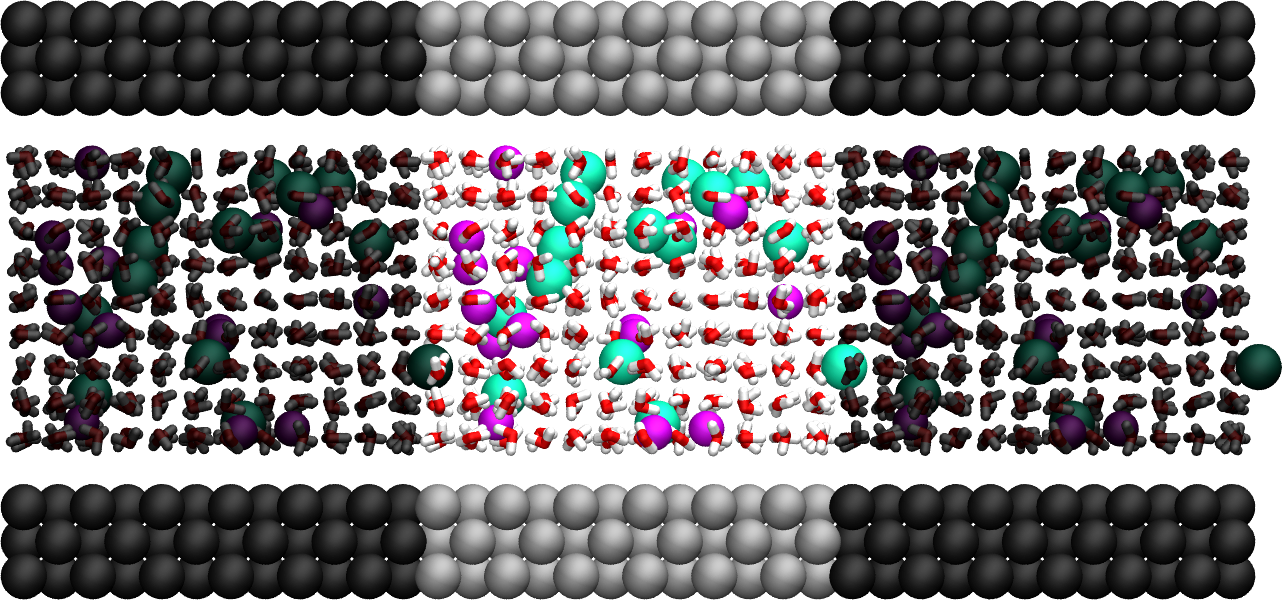
\includegraphics[width=\linewidth]{NANOSHEAR-system}
\caption{Side view of the system. Periodic images are represented in darker colors.
Water molecules are in red and white, $\text{Na}^+$ ions in purple, $\text{Cl}^-$
ions in lime, and wall atoms in gray. Note the absence of atomic defect at the
cell boundaries.}
\label{fig:NANOSHEAR-system}
\end{figure}

\paragraph{Energy minimization}
Let us move the atoms and place them in more energetically favorable positions
before starting the actual molecular dynamics simulation. Let us call this step
\textit{energy minimization}, although it is not a conventional \textit{minimization}
as done for instance in the first tutorial; \hyperref[lennard-jones-label]{Lennard-Jones fluid}.
Instead, a molecular dynamics simulation will be performed here, with some techniques
employed to prevent the system from exploding due to overlapping atoms.

Let us create a new folder called \textit{minimization/} next to \textit{systemcreation/},
and create a new input file called \textit{input.lmp} in it. Copy the following lines
in \textit{input.lmp}:
{\normalsize \begin{verbatim}
boundary p p f
units real
atom_style full
bond_style harmonic
angle_style harmonic
pair_style lj/cut/tip4p/long 1 2 1 1 &
    0.1546 12.0
kspace_style pppm/tip4p 1.0e-4
kspace_modify slab 3.0

read_data ../systemcreation/system.data

include ../PARM.lmp
include ../GROUP.lmp
\end{verbatim}}
The only difference from the previous input is that instead of creating a new
box and new atoms, we open the previously created file \textit{system.data}
located in \textit{systemcreation/}. The file \textit{system.data} contains the
definition of the simulation box and the positions of the atoms.

Now, let us create a first simulation step using a relatively small
timestep ($0.5\,\text{fs}$) and a low temperature of $T = 1\,\text{K}$:
{\normalsize \begin{verbatim}
fix mynve fluid nve/limit 0.1
fix myber fluid temp/berendsen 1 1 100
fix myshk H2O shake 1.0e-4 200 0 b O-H a H-O-H
timestep 0.5
\end{verbatim}}
Just like \textit{fix nve}, the \textit{fix nve/limit} command performs constant
NVE integration to update the positions and velocities of the atoms at each
timestep. The difference is that \textit{fix nve/limit} also limits the maximum
distance atoms can travel at each timestep. Here, the chosen maximum distance
is $0.1~\text{\AA{}}$. Because the \textit{fix nve/limit} is applied to the
group \textit{fluid}, only the water molecules and ions will move.
The \textit{fix temp/berendsen} rescales the velocities of the atoms to
force the temperature of the system to reach the desired value of $1~\text{K}$,
and the SHAKE algorithm is used in order to maintain the shape of the water molecules.

Let us also create images of the system and control
the printing of thermodynamic outputs by adding the following lines to \textit{input.lmp}:
{\normalsize \begin{verbatim}
dump mydmp all image 200 dump.*.jpg type type &
    shiny 0.1 box no 0.01 view 90 0 zoom 1.8
dump_modify mydmp backcolor white &
    acolor O red adiam O 2 &
    acolor H white adiam H 1 &
    acolor Na+ blue adiam Na+ 2.5 &
    acolor Cl- cyan adiam Cl- 3 &
    acolor WALL gray adiam WALL 3
thermo 200
\end{verbatim}}
Finally, let us run for 4000 steps. Add the following lines into \textit{input.lmp}:
{\normalsize \begin{verbatim}
run 4000
\end{verbatim}}
When running the \textit{input.lmp} file with LAMMPS, you should see that the
total energy of the system is initially very high, but rapidly decreases and
reach a plateau (Fig.\,\ref{fig:NANOSHEAR-minimization}). From the generated image of the system,
you will see that some of the atoms are moving, particularly those that were
initially in problematic positions.

In order to better equilibrate the system, let us perform two additional steps
with a larger timestep and a higher imposed temperature:
{\normalsize \begin{verbatim}
fix myber fluid temp/berendsen 300 300 100
timestep 1.0

run 4000

unfix mynve
fix mynve fluid nve

run 4000

write_data system.data nocoeff
\end{verbatim}}
For the last of the three steps, fix \textit{nve} is used instead of
\textit{nve/limit}, which will allow for better relaxation of the atom positions.

When running the \textit{input.lmp} file with LAMMPS, you should see that the
the temperature reaches the desired value of $300\,\text{K}$. The generated file
\textit{system.data} contains the final state of the system.

\begin{figure}
\centering
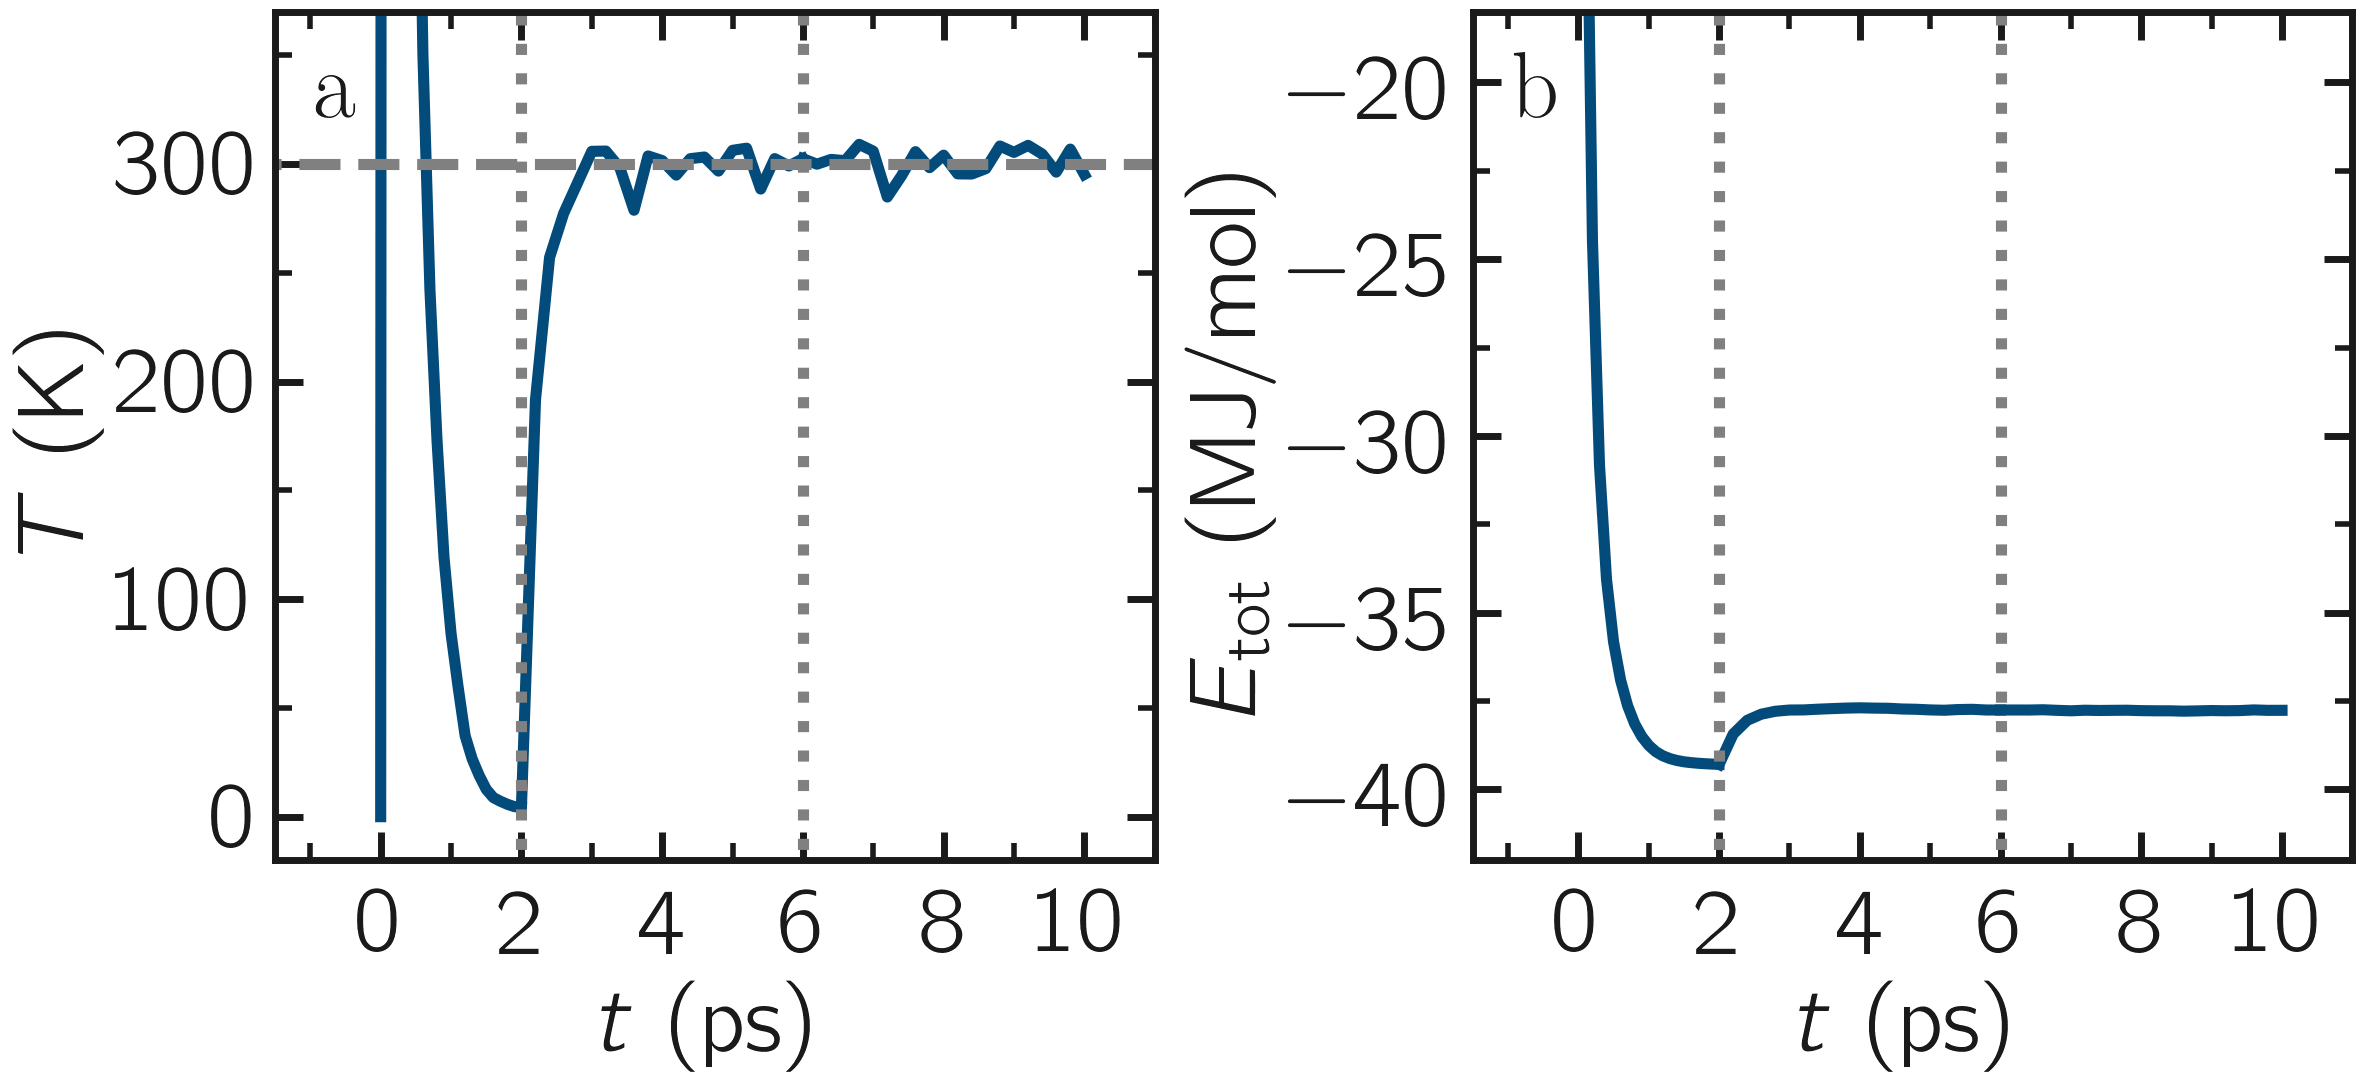
\includegraphics[width=\linewidth]{NANOSHEAR-minimization}
\caption{Total energy of the system $E_\text{tot}$ as a function of time $t$
extracted from the log file using \textit{Python} and \textit{lammps\_logfile}
\cite{sveinsson2021logfile}. The vertical dashed lines demarcate the three
consecutive steps.}
\label{fig:NANOSHEAR-minimization}
\end{figure}

\paragraph{System equilibration}
Let us equilibrate further the entire system by letting both fluid and piston
relax at ambient temperature. Create a new folder called \textit{equilibration/}
next to the previously created folders, and create a new \textit{input.lmp}
file in it. Add the following lines into \textit{input.lmp}:
{\normalsize \begin{verbatim}
boundary p p f
units real
atom_style full
bond_style harmonic
angle_style harmonic
pair_style lj/cut/tip4p/long 1 2 1 1 &
    0.1546 12.0
kspace_style pppm/tip4p 1.0e-4
kspace_modify slab 3.0

read_data ../minimization/system.data

include ../PARM.lmp
include ../GROUP.lmp

fix mynve all nve
fix myber all temp/berendsen 300 300 100
fix myshk H2O shake 1.0e-4 200 0 b O-H a H-O-H
fix myrct all recenter NULL NULL 0
timestep 1.0
\end{verbatim}}
The fix \textit{recenter} does not influence the dynamics but will keep the
system in the center of the box, which makes the
visualization easier. Then, add the following lines into \textit{input.lmp}
for the trajectory visualization and output:
{\normalsize \begin{verbatim}

dump mydmp all image 200 dump.*.jpg type type &
    shiny 0.1 box no 0.01 view 90 0 zoom 1.8
dump_modify mydmp backcolor white &
    acolor O red adiam O 2 &
    acolor H white adiam H 1 &
    acolor Na+ blue adiam Na+ 2.5 &
    acolor Cl- cyan adiam Cl- 3 &
    acolor WALL gray adiam WALL 3
thermo 500
variable walltopz equal xcm(walltop,z)
variable wallbotz equal xcm(wallbot,z)
variable deltaz equal v_walltopz-v_wallbotz
fix myat1 all ave/time 100 1 100 v_deltaz &
    file interwall_distance.dat
\end{verbatim}}
The first two variables extract the centers of mass of the two walls. Then,
the \textit{deltaz} variable is used to calculate the distance between the two
variables \textit{walltopz} and \textit{wallbotz}, i.e. the distance between the two walls.

Finally, let us add the \textit{run} command:
{\normalsize \begin{verbatim}
run 30000
write_data system.data nocoeff
\end{verbatim}}
Run the \textit{input.lmp} file using LAMMPS. As seen from the data printed by
\textit{fix myat1}, the distance between the two walls reduces until it reaches
an equilibrium value (Fig.\,\ref{fig:NANOSHEAR-equilibration}).

Note that it is generally recommended to run longer equilibration. Here, for
instance, the slowest process in the system is probably the ionic diffusion.
Therefore, the equilibration should in principle be longer than the time
the ions need to diffuse over the size of the pore ($\approx 1.2\,\text{nm}$),
i.e. on the order of half a nanosecond.

\begin{figure}
\centering
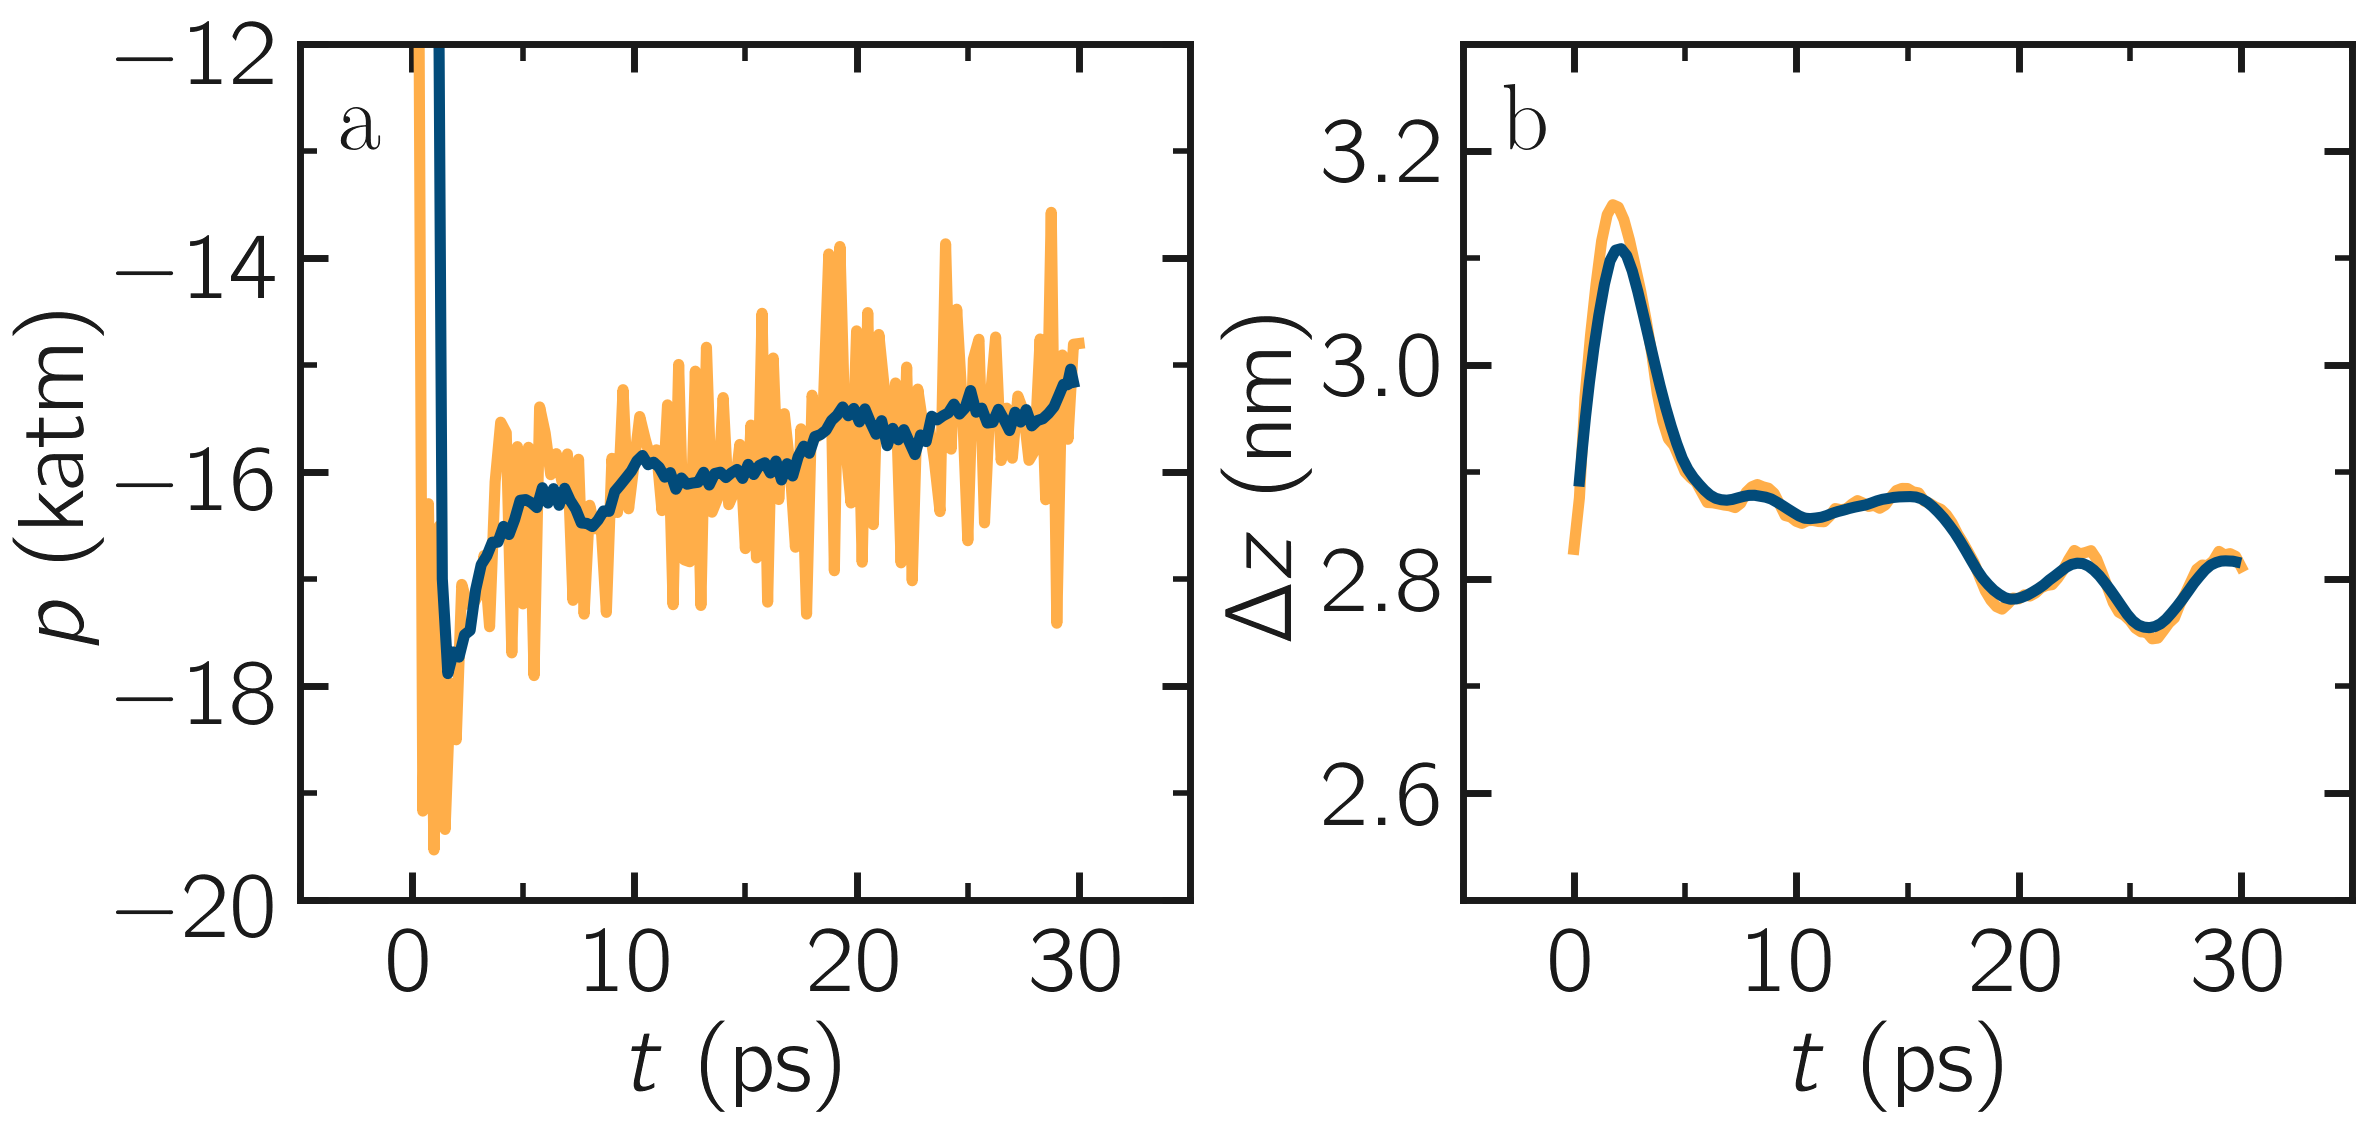
\includegraphics[width=\linewidth]{NANOSHEAR-equilibration}
\caption{Distance between the walls $d$ as a function of time $t$.}
\label{fig:NANOSHEAR-equilibration}
\end{figure}

\subsubsection{Imposed shearing}

From the equilibrated configuration, let us impose a lateral motion on the two
walls and shear the electrolyte. In a new folder called \textit{shearing/},
create a new \textit{input.lmp} file that starts like the previous ones:
{\normalsize \begin{verbatim}
boundary p p f
units real
atom_style full
bond_style harmonic
angle_style harmonic
pair_style lj/cut/tip4p/long 1 2 1 1 &
    0.1546 12.0
kspace_style pppm/tip4p 1.0e-4
kspace_modify slab 3.0
\end{verbatim}}
Let us import the previously equilibrated data, include the parameter and group
files, and then deal with the dynamics of the system.
{\normalsize \begin{verbatim}
read_data ../equilibration/system.data

include ../PARM.lmp
include ../GROUP.lmp

fix mynve all nve
compute Tfluid fluid temp/partial 0 1 1
fix myber1 fluid temp/berendsen 300 300 100
fix_modify myber1 temp Tfluid
compute Twall wall temp/partial 0 1 1
fix myber2 wall temp/berendsen 300 300 100
fix_modify myber2 temp Twall
fix myshk H2O shake 1.0e-4 200 0 b O-H a H-O-H
fix myrct all recenter NULL NULL 0
\end{verbatim}}
One difference with the previous input is that, here, two thermostats are used,
one for the fluid (\textit{myber1}) and one for the solid (\textit{myber2}).
The use of \textit{fix\_modify} together with \textit{compute temp} ensures
that the right temperature value is used by the thermostats. The use of
temperature \textit{compute} with \textit{temp/partial 0 1 1} is meant to exclude
the \textit{x} coordinate from the thermalization, which is important since a
large velocity will be imposed along \textit{x}.

Then, let us impose the velocity of the two walls by adding the following
commands to \textit{input.lmp}:
{\normalsize \begin{verbatim}
fix mysf1 walltop setforce 0 NULL NULL
fix mysf2 wallbot setforce 0 NULL NULL
velocity wallbot set -2e-4 NULL NULL
velocity walltop set 2e-4 NULL NULL
\end{verbatim}}
The \textit{setforce} commands cancel the forces on \textit{walltop} and
\textit{wallbot}, respectively. Therefore the atoms of the two groups do not
experience any force from the rest of the system. In the absence of force acting
on those atoms, they will conserve their initial velocity. The \textit{velocity}
commands act only once and impose the velocity of the atoms of the groups
\textit{wallbot} and \textit{walltop}, respectively.

Finally, let us dump the atom positions, and extract the velocity profiles using
several \textit{ave/chunk} commands, extract the force applied on the walls, and
then run for $200\,\text{ps}$ Add the following lines into \textit{input.lmp}:
{\normalsize \begin{verbatim}
dump mydmp all image 200 dump.*.jpg type type &
    shiny 0.1 box no 0.01 view 90 0 zoom 1.8
dump_modify mydmp backcolor white &
    acolor O red adiam O 2 &
    acolor H white adiam H 1 &
    acolor Na+ blue adiam Na+ 2.5 &
    acolor Cl- cyan adiam Cl- 3 &
    acolor WALL gray adiam WALL 3

thermo 500
thermo_modify temp Tfluid

compute cc1 H2O chunk/atom bin/1d z 0.0 1.0
compute cc2 wall chunk/atom bin/1d z 0.0 1.0
compute cc3 ions chunk/atom bin/1d z 0.0 1.0

fix myac1 H2O ave/chunk 10 15000 200000 &
cc1 density/mass vx file water.profile_1A.dat
fix myac2 wall ave/chunk 10 15000 200000 &
cc2 density/mass vx file wall.profile_1A.dat
fix myac3 ions ave/chunk 10 15000 200000 &
cc3 density/mass vx file ions.profile_1A.dat

fix myat1 all ave/time 10 100 1000 f_mysf1[1] &
    f_mysf2[1] file forces.dat

timestep 1.0
run 200000
write_data system.data nocoeff
\end{verbatim}}
Here, a binning of $1\,\text{\AA{}}$ is used for the density profiles generated
by the \textit{ave/chunk} commands. For smoother profiles, you can reduce the value
of the bins. The averaged velocity and density profiles of the fluid are plotted
in Figs.\ref{fig:NANOSHEAR-velocity}-\ref{fig:NANOSHEAR-density}. As expected for
such Couette flow geometry, the velocity of the fluid is found to increase linearly
along $z$.

\begin{figure}
\centering
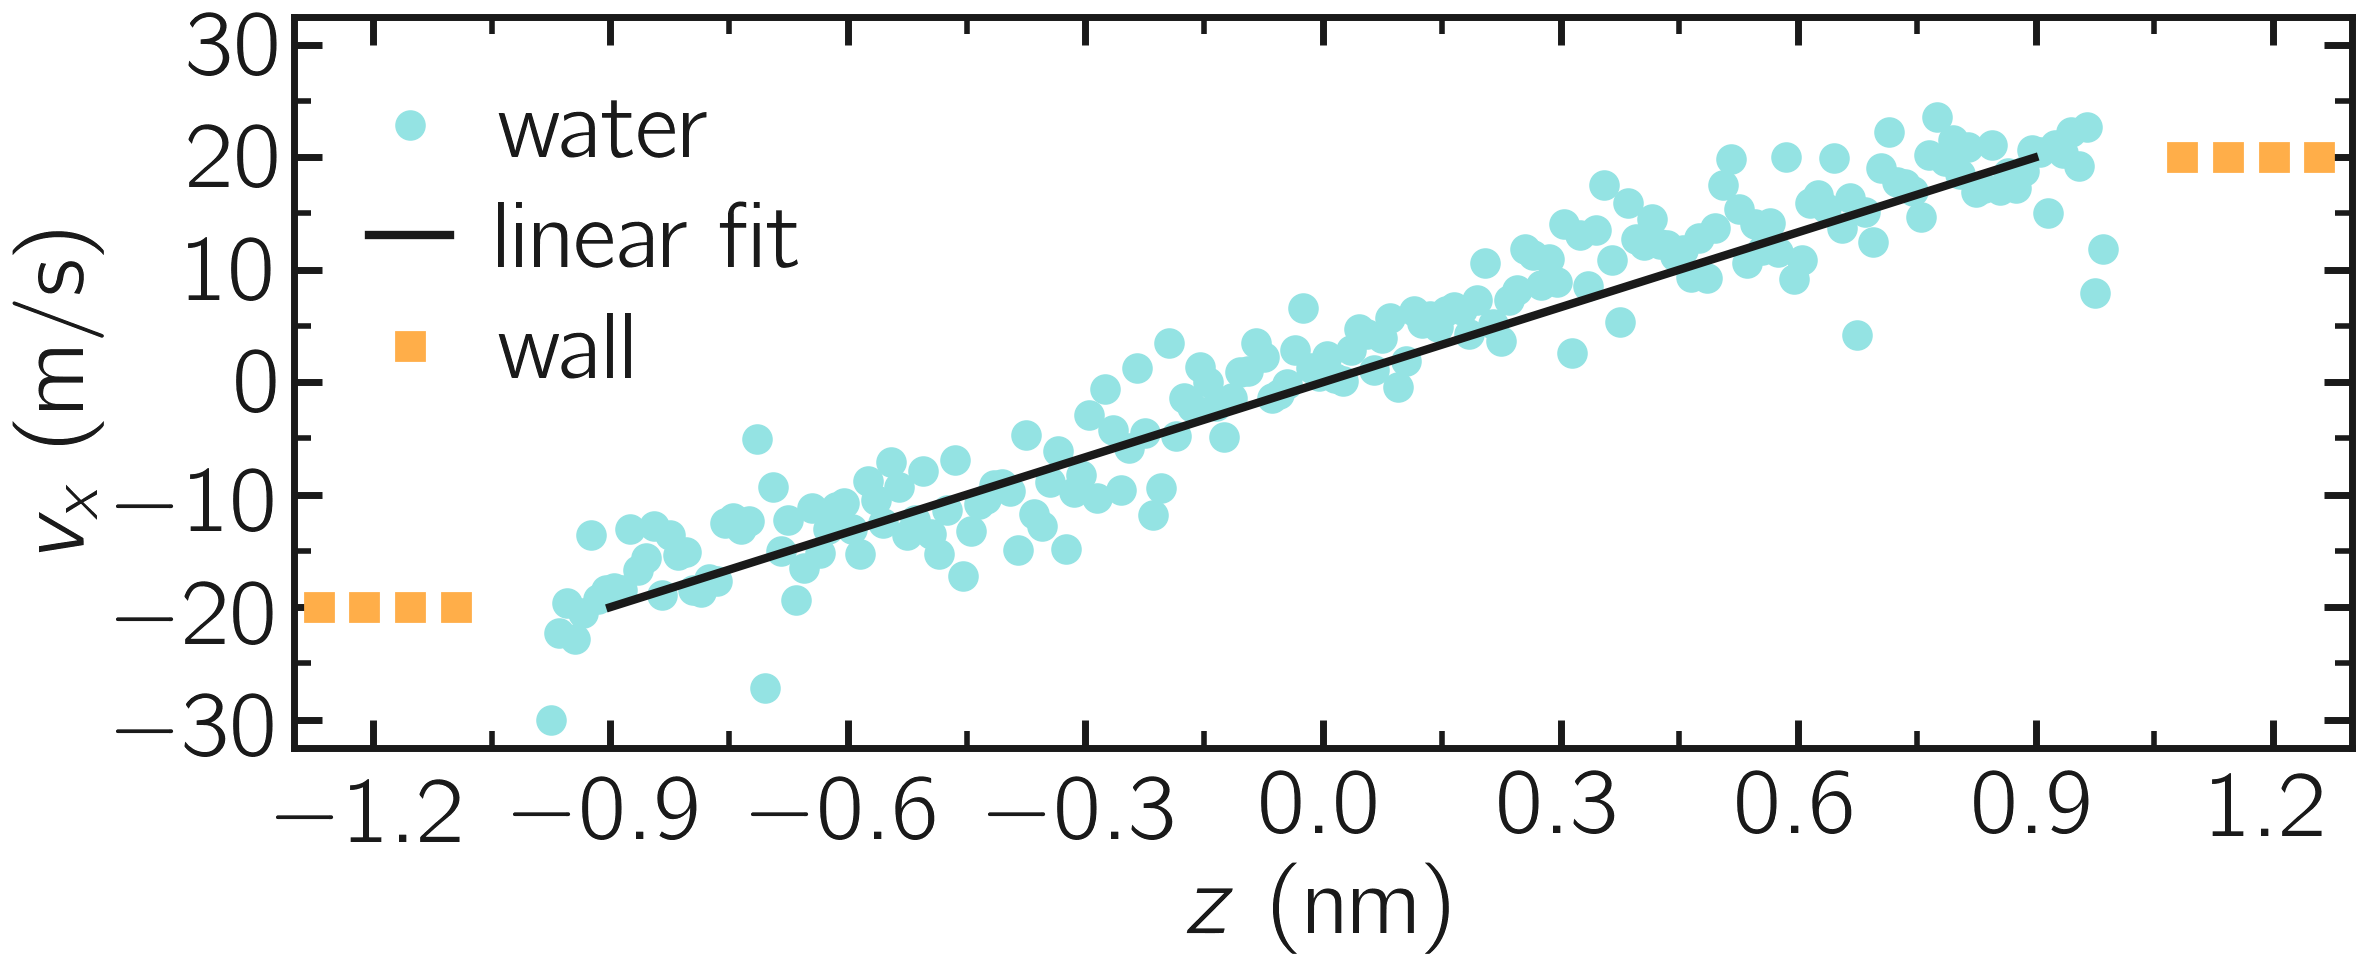
\includegraphics[width=\linewidth]{NANOSHEAR-velocity}
\caption{Velocity profiles for water molecules and ions (blue disks), and walls
(orange squares) along the \textit{z} axis. The line is a linear fit assuming
that the pore size is $h = 1.8\,\text{nm}$.}
\label{fig:NANOSHEAR-velocity}
\end{figure}

\begin{figure}
\centering
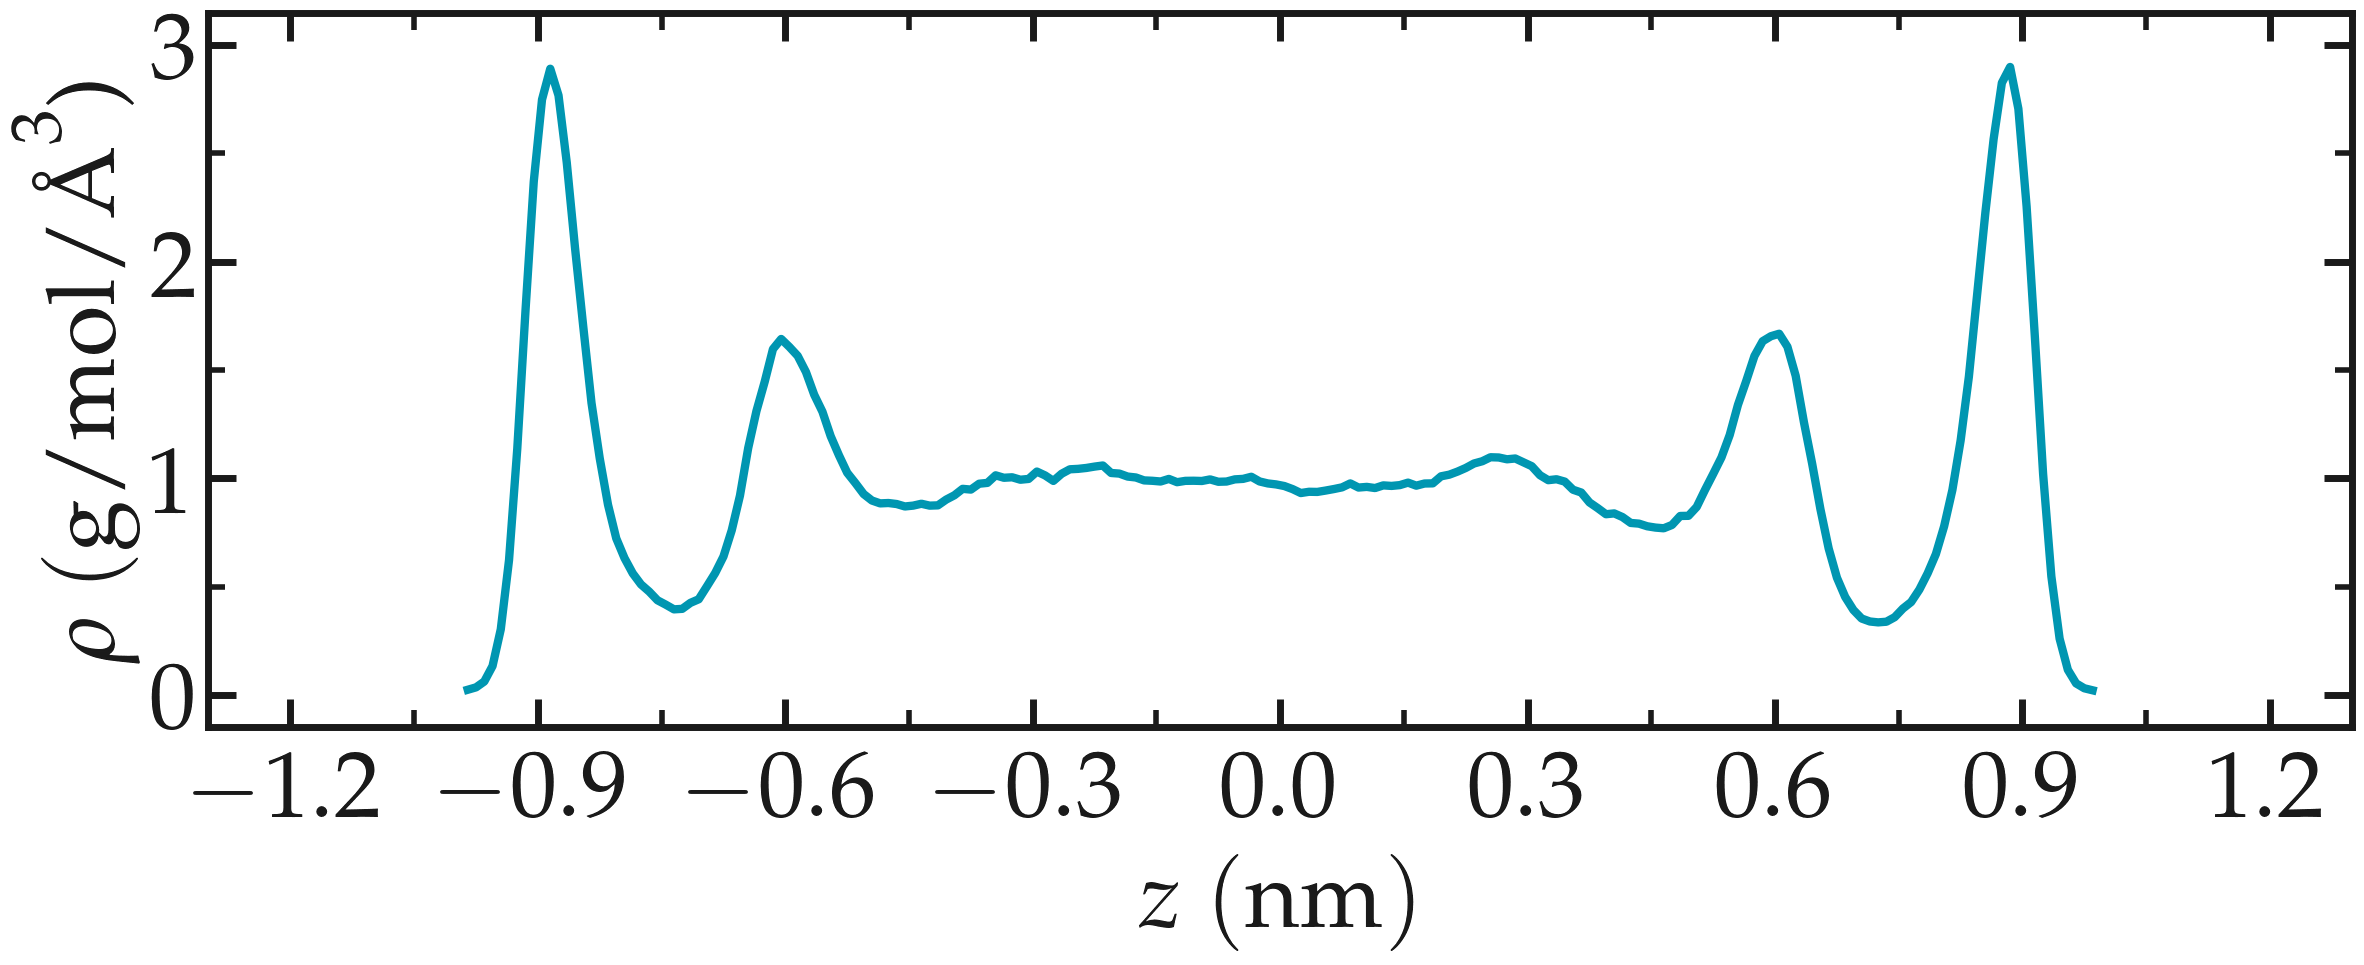
\includegraphics[width=\linewidth]{NANOSHEAR-density}
\caption{Water density $\rho$ along the \textit{z} axis.}
\label{fig:NANOSHEAR-density}
\end{figure}

From the force applied by the fluid on the solid, one can extract the stress
within the fluid, which allows for the measurement of its viscosity $\dot{\eta}$
according to $\eta = \tau / \dot{\gamma}$ where $\tau$ is the stress applied by
the fluid on the shearing wall, and $\dot{\gamma}$ the shear rate (which is
imposed here) \cite{gravelle2021violations}. Here, the shear rate is
approximatively $\dot{\gamma} = 16 \cdot 10^9\,\text{s}^{-1}$, and using a
surface area of $A = 6 \cdot 10^{-18}\,\text{m}^2$, one gets an estimate for
the shear viscosity for the confined fluid of $\eta = 6.6\,\text{mPa.s}$. The
viscosity calculated at such a high shear rate may differ from the expected
\textit{bulk} value. In general, it is recommended to use a lower value for the
shear rate. Note that for lower shear rates, the ratio of noise-to-signal is
larger, and longer simulations are needed. Another important point to keep in
mind is that the viscosity of a fluid next to a solid surface is typically larger
than in bulk due to interaction with the walls \cite{wolde-kidanInterplayInterfacialViscosity2021}.
Therefore, one expects the present simulation to return a viscosity that is slightly
larger than what would be measured in the absence of a wall.

\subsection{Tutorial 5: Reactive silicon dioxide}
\label{reactive-silicon-dioxide-label}

\begin{figure}
\centering
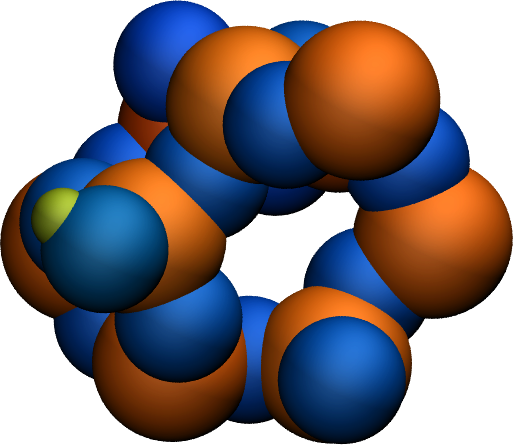
\includegraphics[width=0.55\linewidth]{SIO}
\caption{A portion of the silicon dioxide structure as simulated during
\hyperref[reactive-silicon-dioxide-label]{Tutorial 5}. Atoms are colored by their charges.}
\label{fig:SIO}
\end{figure}

\noindent The objective of this tutorial is to use the reactive force field ReaxFF
to calculate the partial charges of a system undergoing deformation, as well as
the formation and breaking of chemical bonds \cite{van2001reaxff, zou2012investigation}.
The system simulated here is a block of silicon dioxide $\text{SiO}_2$ (Fig.\,\ref{fig:SIO})
that is deformed until rupture. Particular attention is given to the evolution of
the atomic charges during the deformation of the structure, and the chemical
reactions occurring due to the deformation are tracked over time.

\subsubsection{Prepare and relax}
Create a folder, name it \textit{RelaxSilica/}, and download the initial topology
of a small amorphous silica structure called
\href{https://raw.githubusercontent.com/lammpstutorials/lammpstutorials-article/main/files/tutorial5/silica.data}{\textit{silica.data}}.
This structure was created using a classical force field called
Vashishta \cite{vashishta1990interaction}. If you open the \textit{silica.data}
file, you will see in the Atoms section that all silicon atoms have the same
charge $q = 1.1\,\text{e}$, and all oxygen atoms have the charge $q = -0.55\,\text{e}$.
This is common with classical force fields and will change once ReaxFF is used.

The first action we need to perform here is to relax the structure with ReaxFF,
which we are gonna do using molecular dynamics. To make sure that the system
equilibrates nicely, let us track some parameters over time. Create an input
file called \textit{input.lmp} in \textit{RelaxSilica/}, and copy the following
lines into it:
{\normalsize \begin{verbatim}
units real
atom_style full

read_data silica.data

mass 1 28.0855 # Si
mass 2 15.999 # O
\end{verbatim}}
So far, the input is very similar to what was seen in the previous tutorials.
Some basic parameters are defined (\textit{units}, \textit{atom\_style} and \textit{masses}),
and the \textit{.data} file is imported by the \textit{read\_data} command.

Now, let us copy three crucial lines into the \textit{input.lmp} file:
{\normalsize \begin{verbatim}
pair_style reaxff NULL safezone 3.0 mincap 150
pair_coeff * * reaxCHOFe.ff Si O
fix myqeq all qeq/reaxff 1 0.0 10.0 1.0e-6 &
    reaxff maxiter 400
\end{verbatim}}
Here, the \textit{pair\_style reaxff} is used with no control file. The
\textit{safezone} and \textit{mincap} keywords have been added to avoid memory
allocation issues, which sometimes can trigger the segmentation faults and
\textit{bondchk} failed errors. The \textit{pair\_coeff} uses the
\href{https://raw.githubusercontent.com/lammpstutorials/lammpstutorials-article/main/files/tutorial5/reaxCHOFe.ff}{\textit{reaxCHOFe.ff}}
file, which must be downloaded and saved within \textit{RelaxSilica/}. For
consistency with the masses and the \textit{silica.data} file, the atoms of type 1
are set as silicon (Si), and the atoms of type 2 as oxygen (O). Finally, the
\textit{fix qeq/reaxff} is used to perform charge equilibration \cite{rappe1991charge}.
The charge equilibration occurs at every step. The values 0.0 and 10.0 are the
low and the high cutoffs, respectively, and $1.0 \text{e} -6$ is a tolerance.
Finally, \textit{maxiter} sets an upper limit to the number of attempts to
equilibrate the charge.

Then, let us add some commands to the \textit{input.lmp} file  to measure the
evolution of the charges during the simulation:
{\normalsize \begin{verbatim}
group grpSi type 1
group grpO type 2
variable qSi equal charge(grpSi)/count(grpSi)
variable qO equal charge(grpO)/count(grpO)
\end{verbatim}}
Let us also print the charge in the \textit{.log} file by using \textit{thermo\_style},
and create images of the system. Add the following lines into the \textit{input.lmp}:
{\normalsize \begin{verbatim}
thermo 200
thermo_style custom step temp etotal press &
    vol v_qSi v_qO
dump mydmp all image 200 dump.*.jpg type type &
    shiny 0.1 box no 0.01 view 0 0 zoom 1.8
dump_modify mydmp backcolor white &
    acolor 1 yellow adiam 1 2.5 &
    acolor 2 red adiam 2 2
\end{verbatim}}

In order to also visualize the system using an external tool, VMD, let us also
create a \textit{.lammpstrj} file for visualization:
{\normalsize \begin{verbatim}
dump dmp all custom 200 dump.lammpstrj &
    id type q x y z
\end{verbatim}}
The \textit{.lammpstrj} that will be created when running lammps will contain
6 columns with respectively the atom IDs, the atom types, the atom charges ($q$),
and finally the atom coordinates ($x$, $y$, and $z$).

Let us also use the \textit{fix reaxff/species} to evaluate what species are
present within the simulation. It will be useful later when the system is deformed
and some bonds are broken:
{\normalsize \begin{verbatim}
fix myspec all reaxff/species 5 1 5 &
    species.log element Si O
\end{verbatim}}
Here, the information will be printed every 5 steps in a file called \textit{species.log}.
Let us perform a very short run using the anisotropic NPT command and relax the
density of the system.
{\normalsize \begin{verbatim}
velocity all create 300.0 3482028
fix mynpt all npt temp 300.0 300.0 100 &
    aniso 1.0 1.0 1000
timestep 0.5

run 5000

write_data silica-relaxed.data
\end{verbatim}}
Run the \textit{input.lmp} file using LAMMPS. As seen from \textit{species.log},
only one species is detected, called O384Si192, representing the entire system.
The value of the charge of the atoms can be extracted from the \textit{dump.lammpstrj}
file using Python. You can use this
\href{https://raw.githubusercontent.com/lammpstutorials/lammpstutorials-article/main/files/tutorial5/dump-reader.py}{\textit{dump-reader}}
script to import the charge values into Python.
As the simulation progresses, the charge of every atom fluctuates
because it is adjusting to the local environment of the atom (Fig.\,\ref{fig:SIO-charge}).
It can also be seen that the averaged charges for both silicon and oxygen
atoms vary abruptly at the beginning of the simulation, which correlates with
a rapid volume change of the box during which the inter-atomic distances are
expected to quickly change (Fig.\,\ref{fig:SIO-volume}).

\begin{figure}
\centering
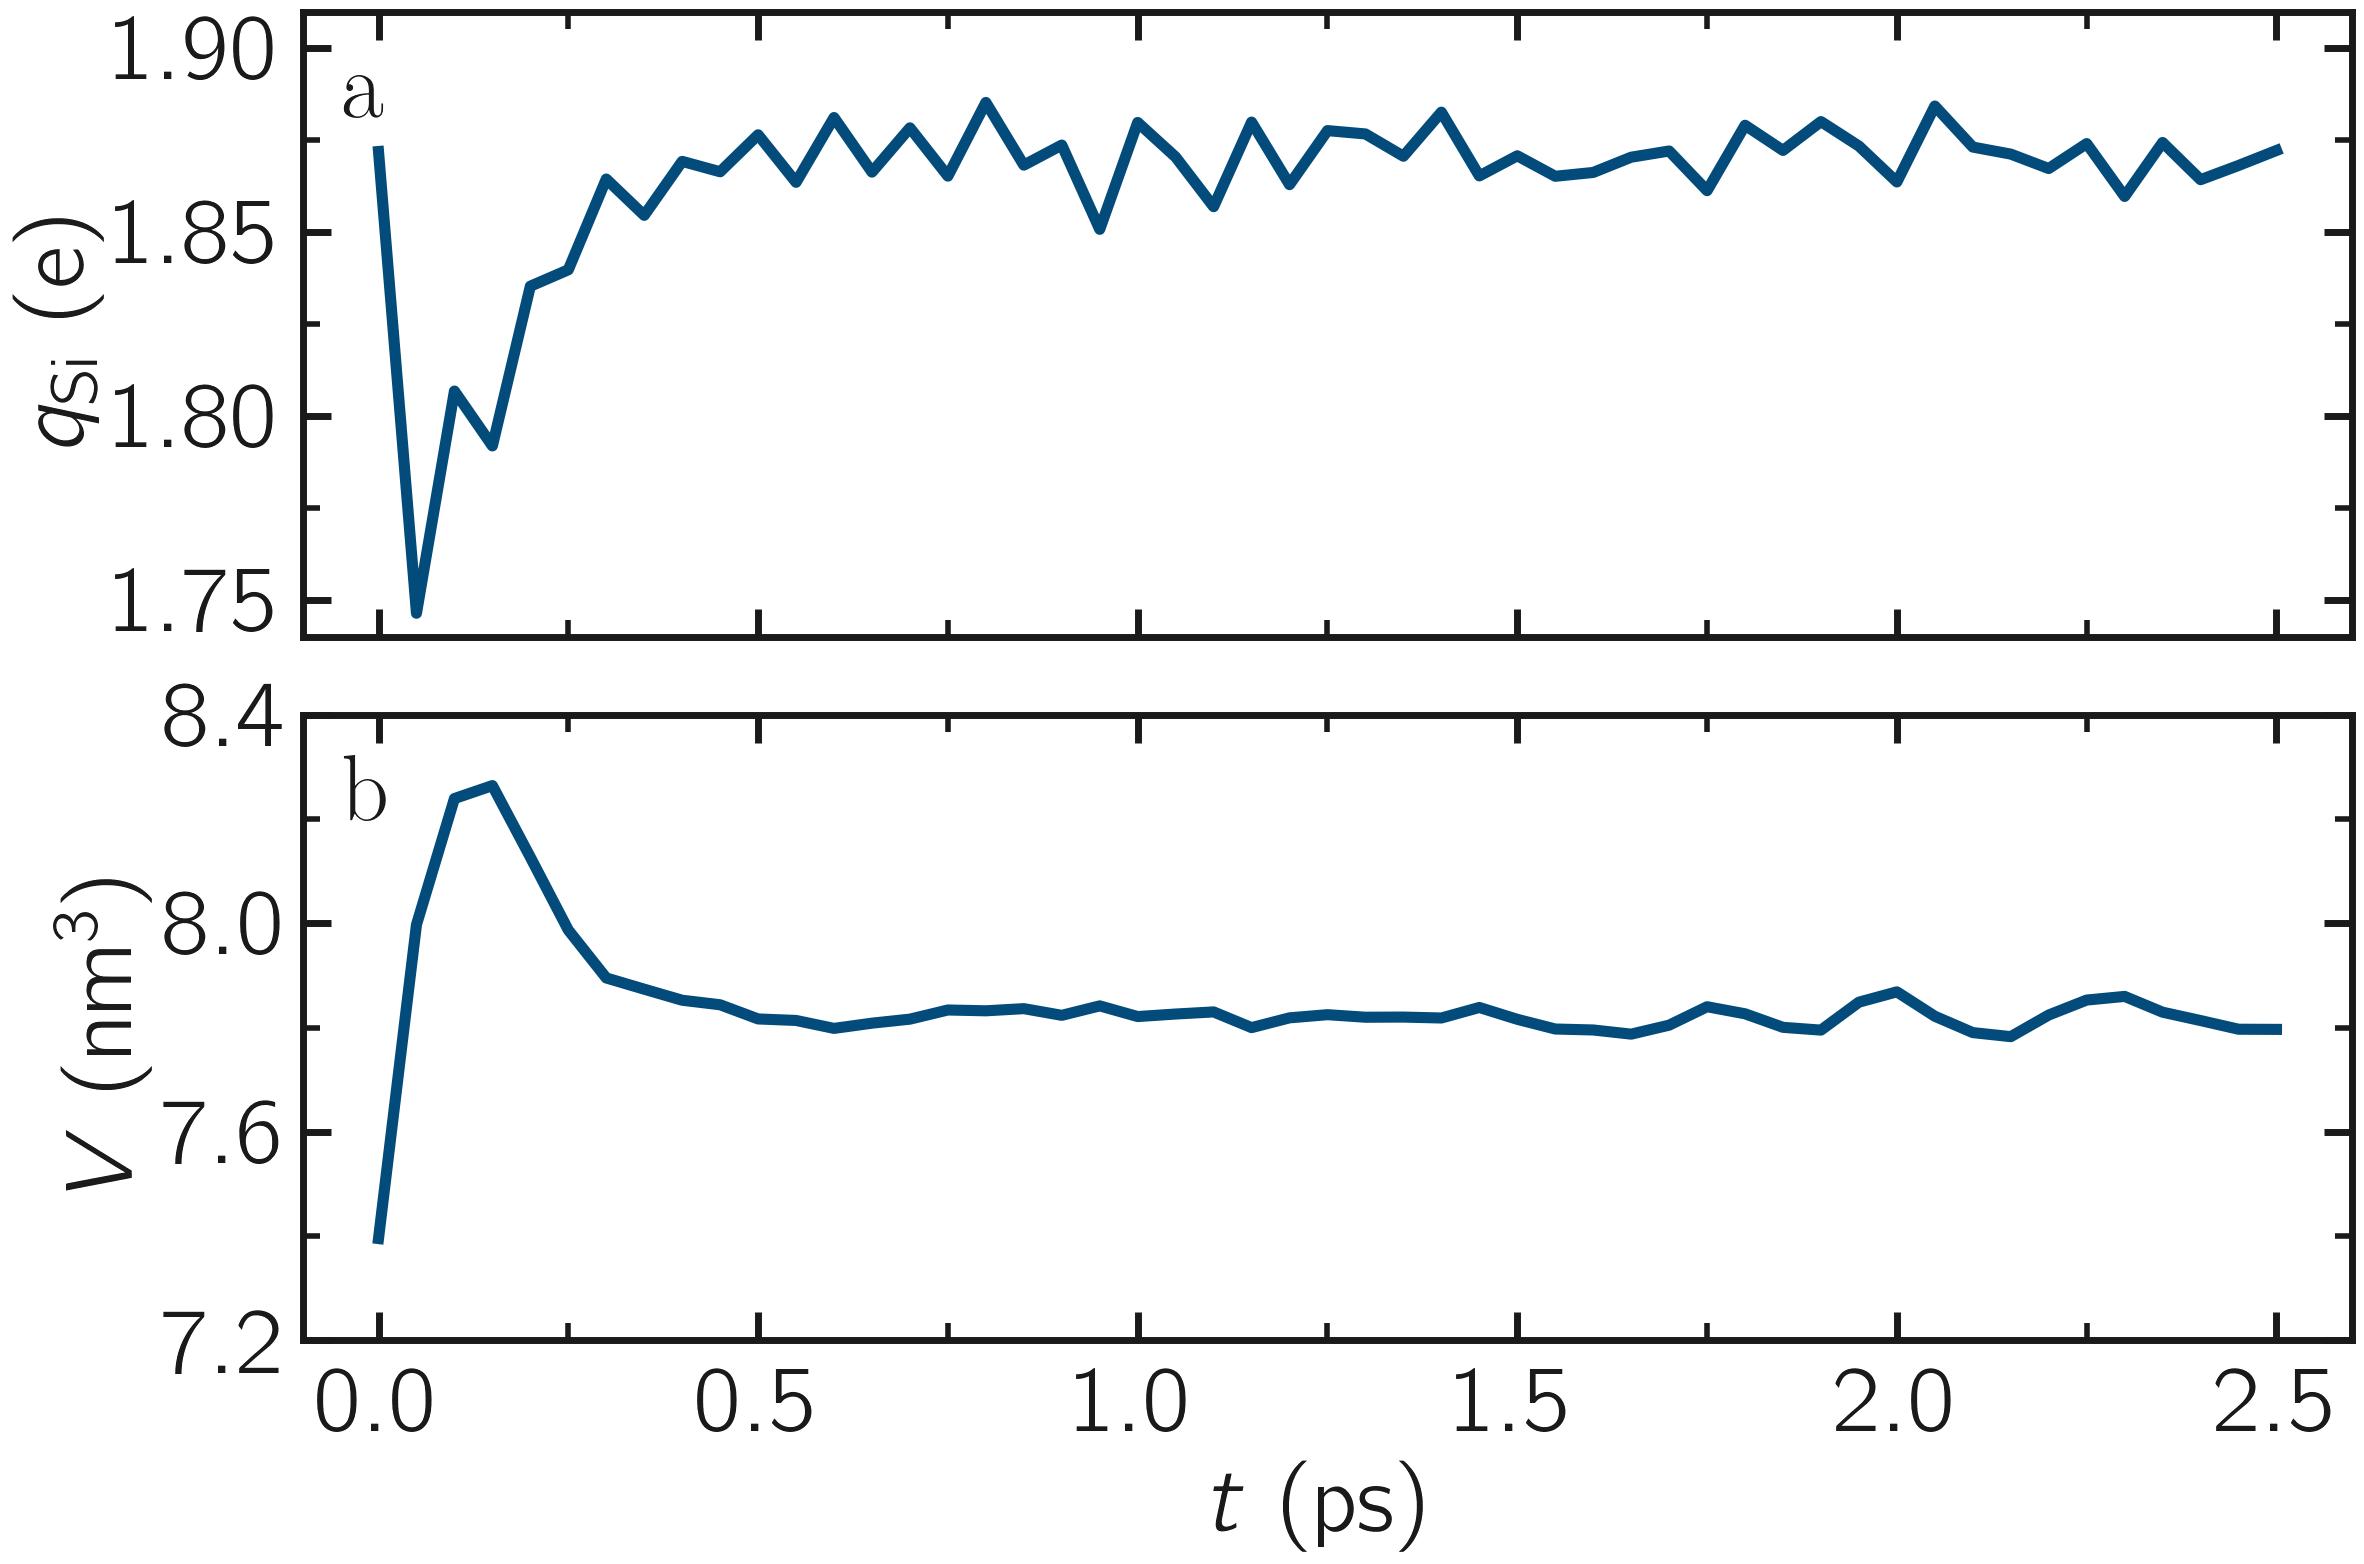
\includegraphics[width=\linewidth]{SIO-charge}
\caption{Average charge per atom of the silicon $q_\text{Si}$ (a) and oxygen
$q_\text{O}$ (b) atoms as a function of time $t$ during equilibration.  $q_\text{Si}$
and $q_\text{O}$ are given by the \textit{v\_qSi} and \textit{v\_qO} variables,
respectively.}
\label{fig:SIO-charge}
\end{figure}

\begin{figure}
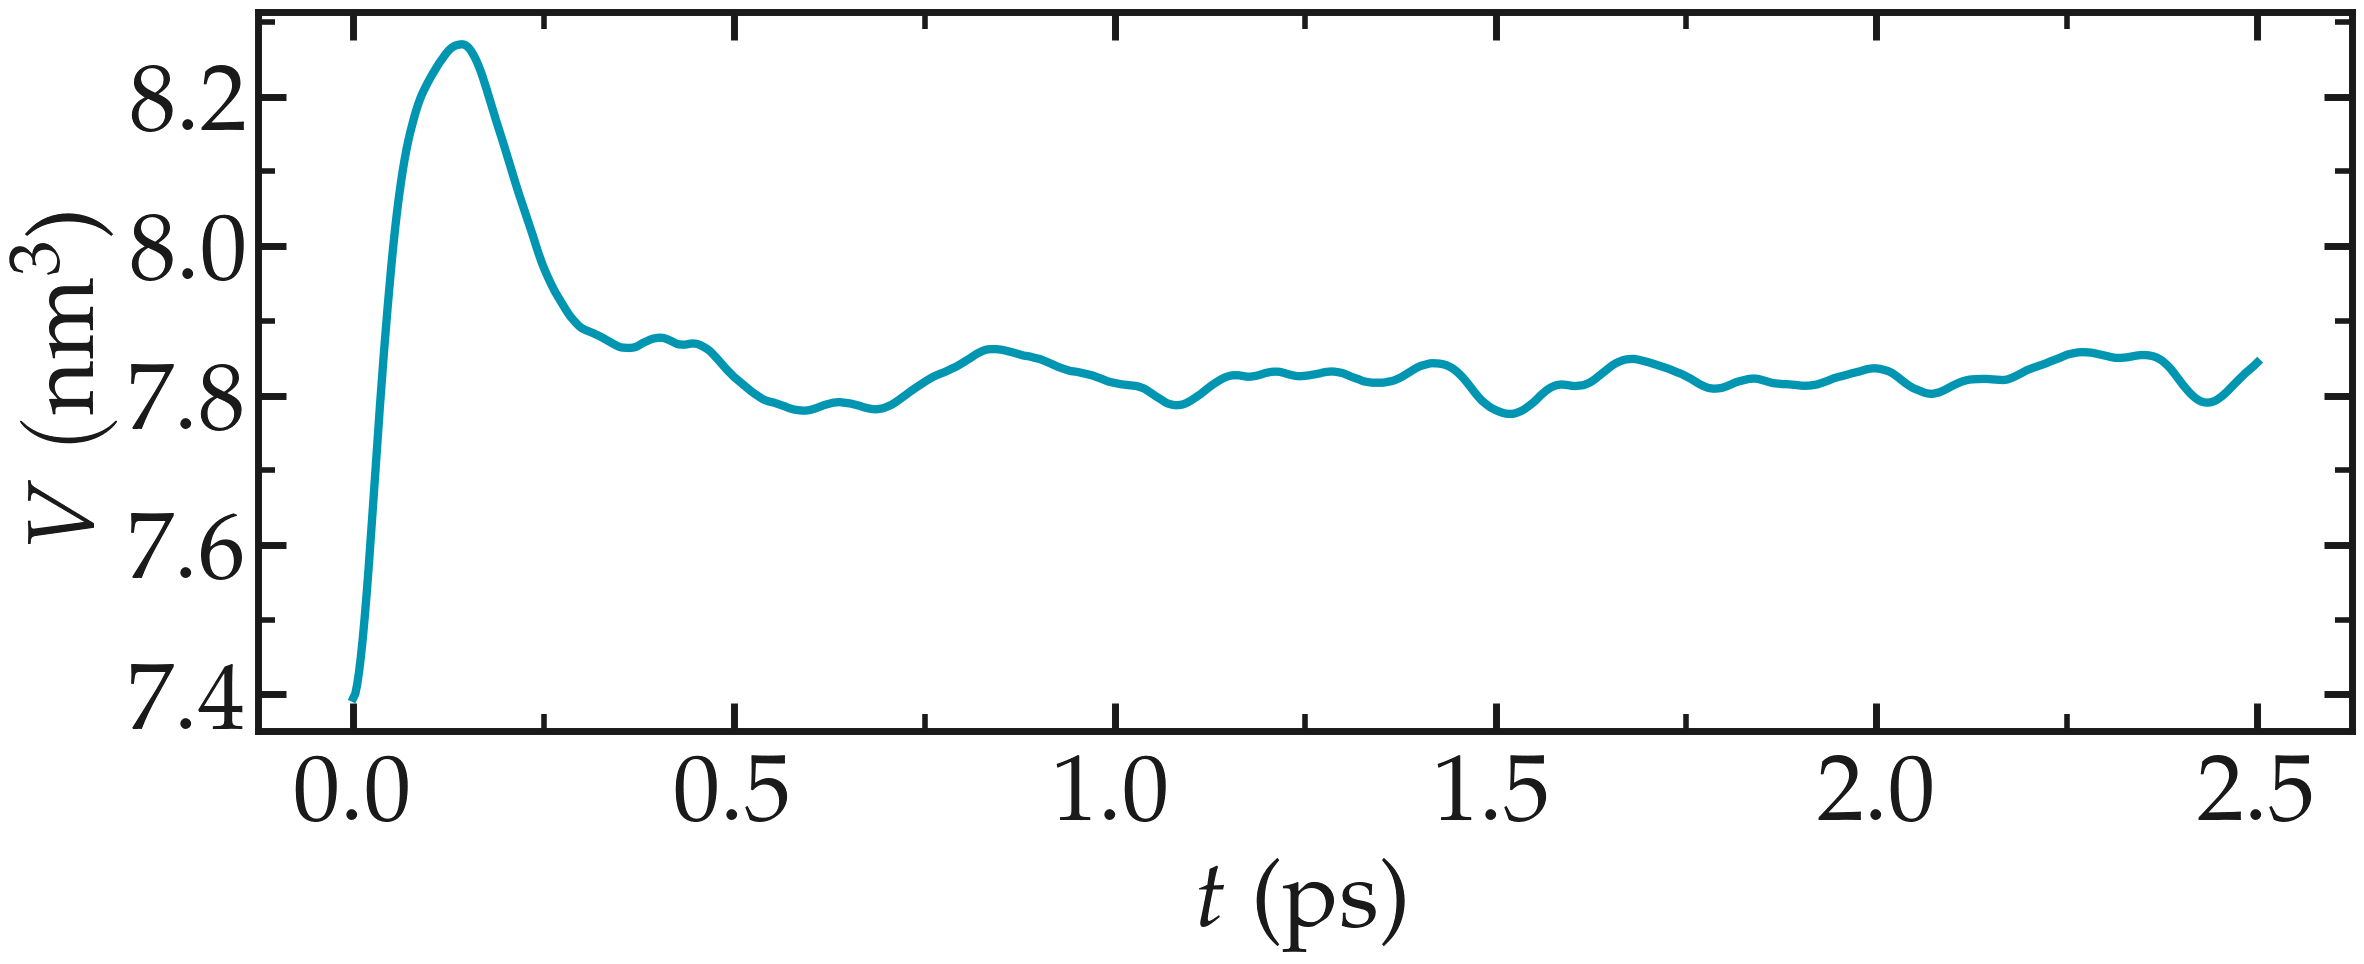
\includegraphics[width=\linewidth]{SIO-volume}
\caption{Volume of the system $V$ as a function of time $t$.}
\label{fig:SIO-volume}
\end{figure}

We can also plot the charge distribution $P(q)$, using the charge values
printed in the \textit{dump.lammptrj} file (Fig.\,\ref{fig:SIO-distribution}).
The \textit{dump.lammptrj} file can be opened using VMD. By coloring the atoms
by their charges, one can see that the atoms with the extreme-most charges are
located at defects in the amorphous structure (here at the positions of the
dangling oxygen groups) (Fig.\,\ref{fig:SIO-slice}).

\begin{figure}
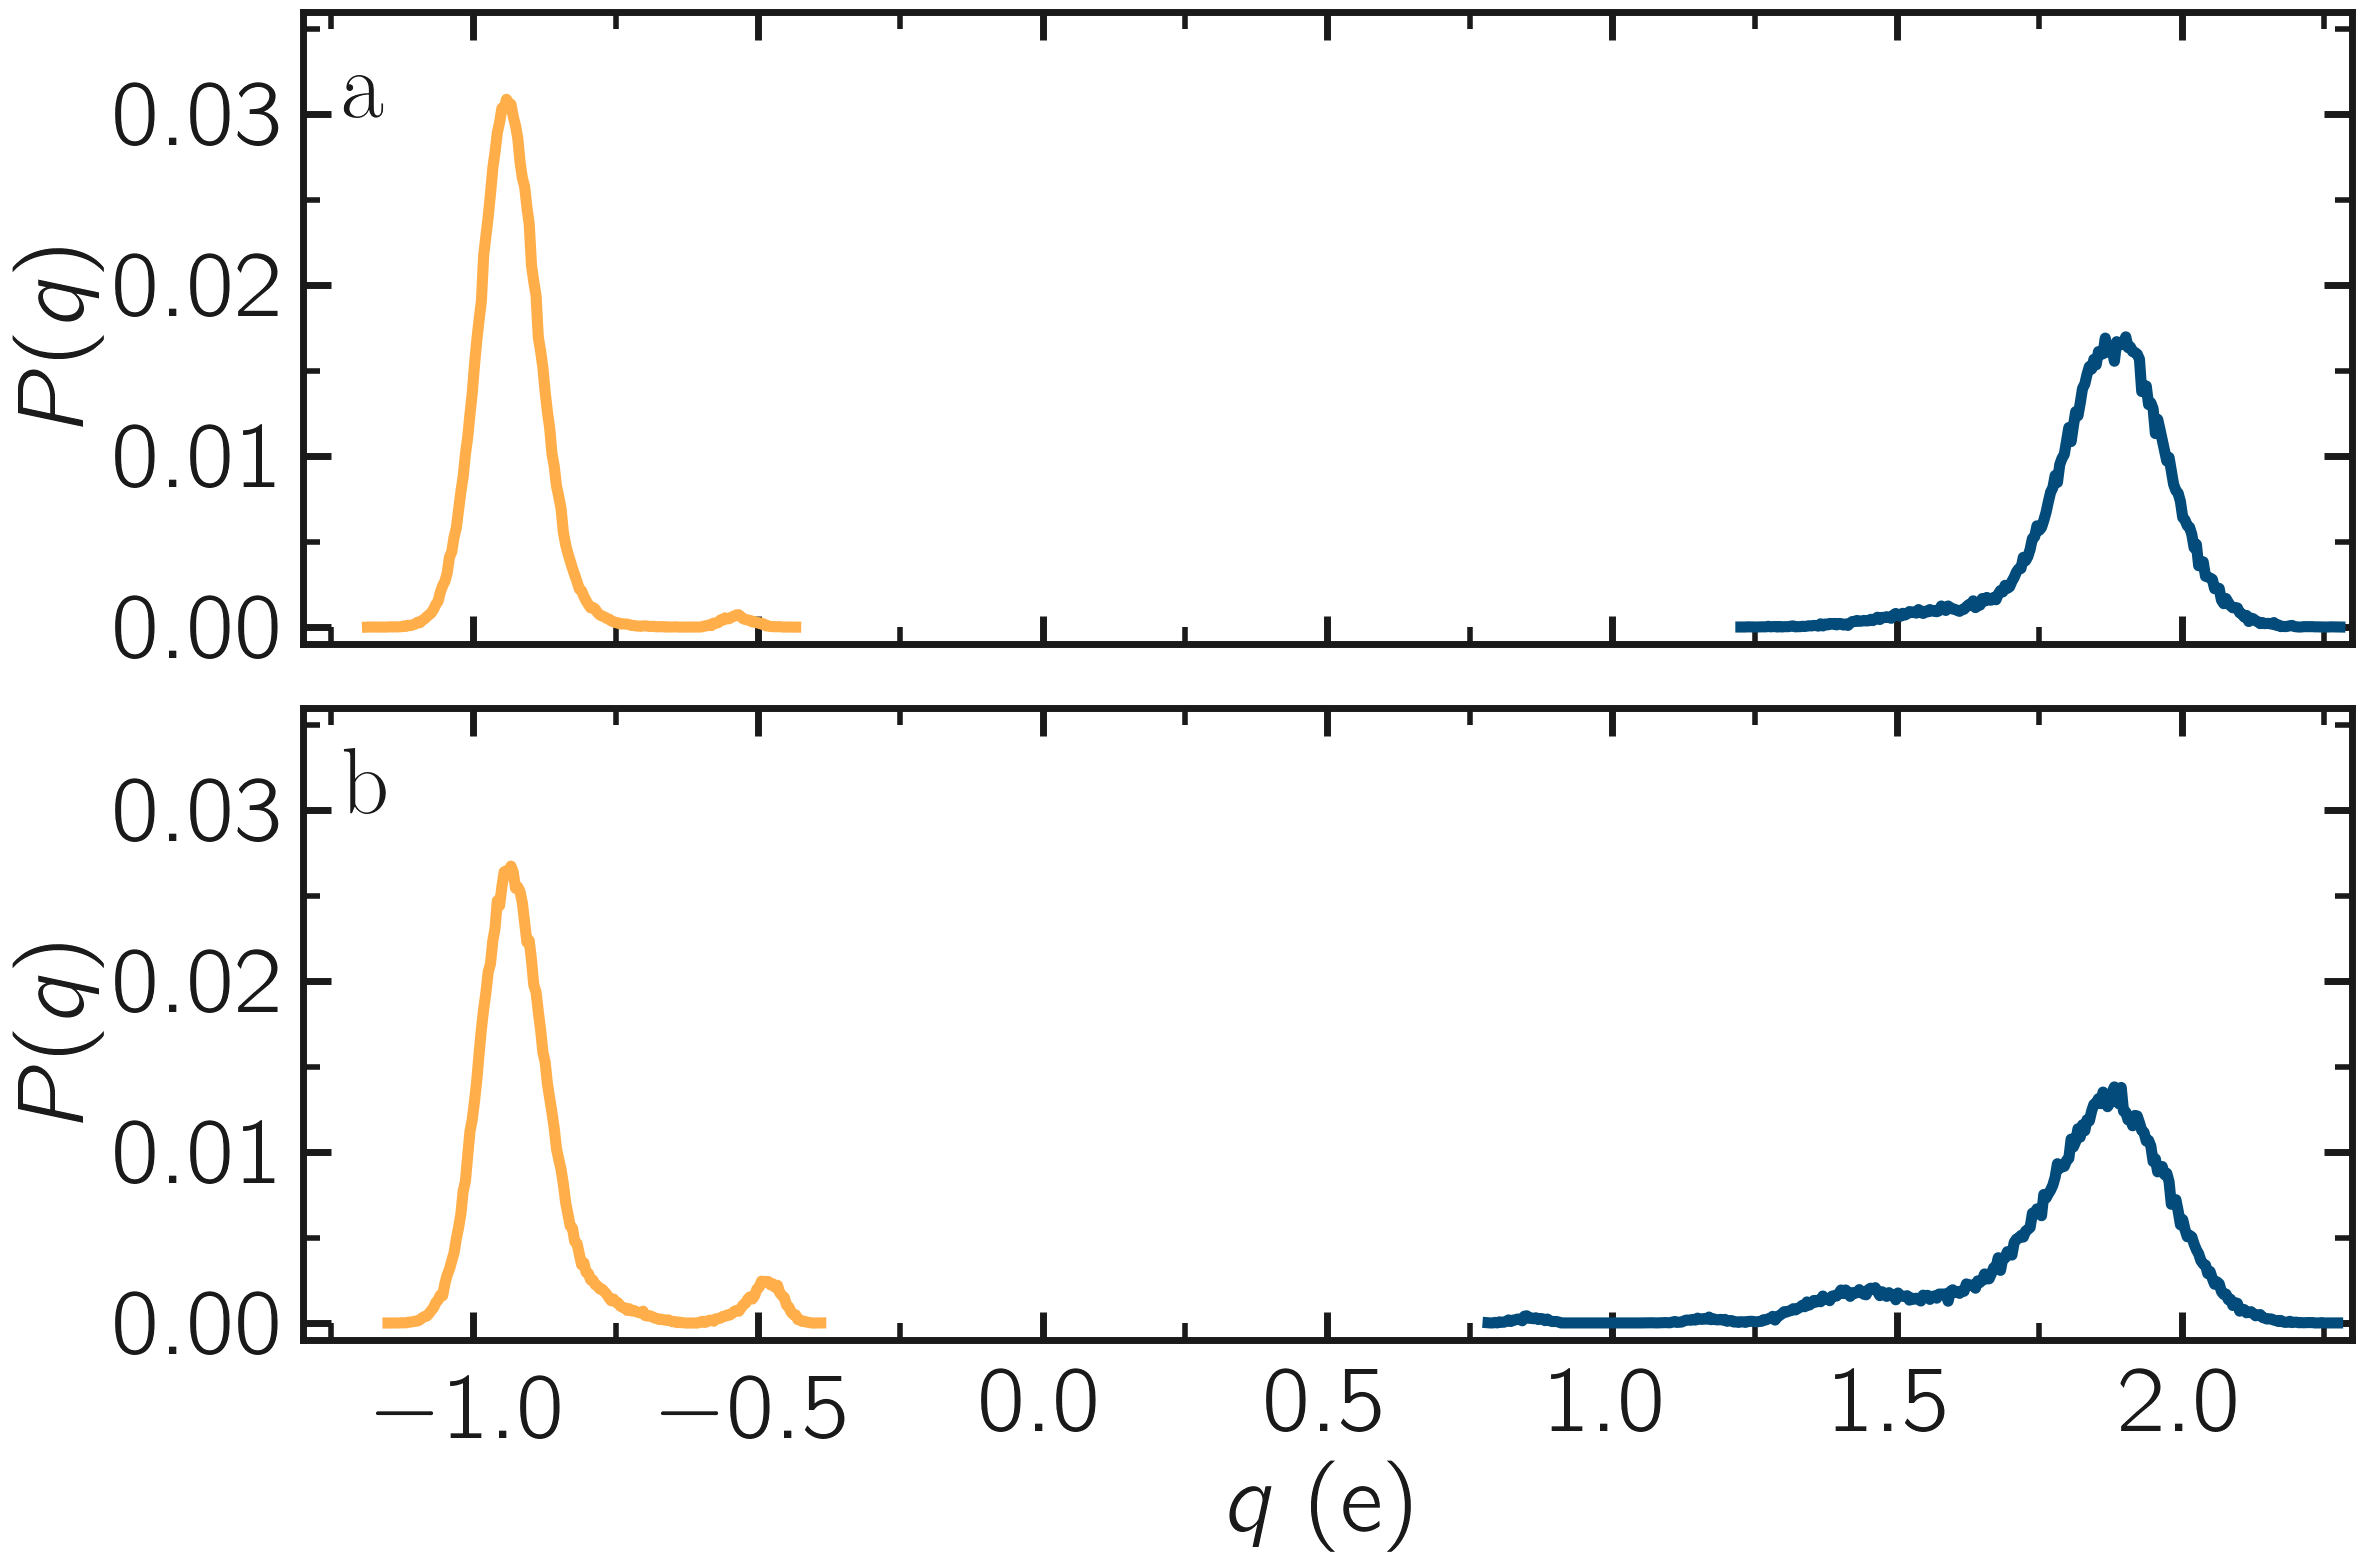
\includegraphics[width=\linewidth]{SIO-distribution}
\caption{Probability distribution of charge of silicon (positive, blue) and oxygen
(negative, orange) atoms during equilibration.}
\label{fig:SIO-distribution}
\end{figure}

\begin{figure}
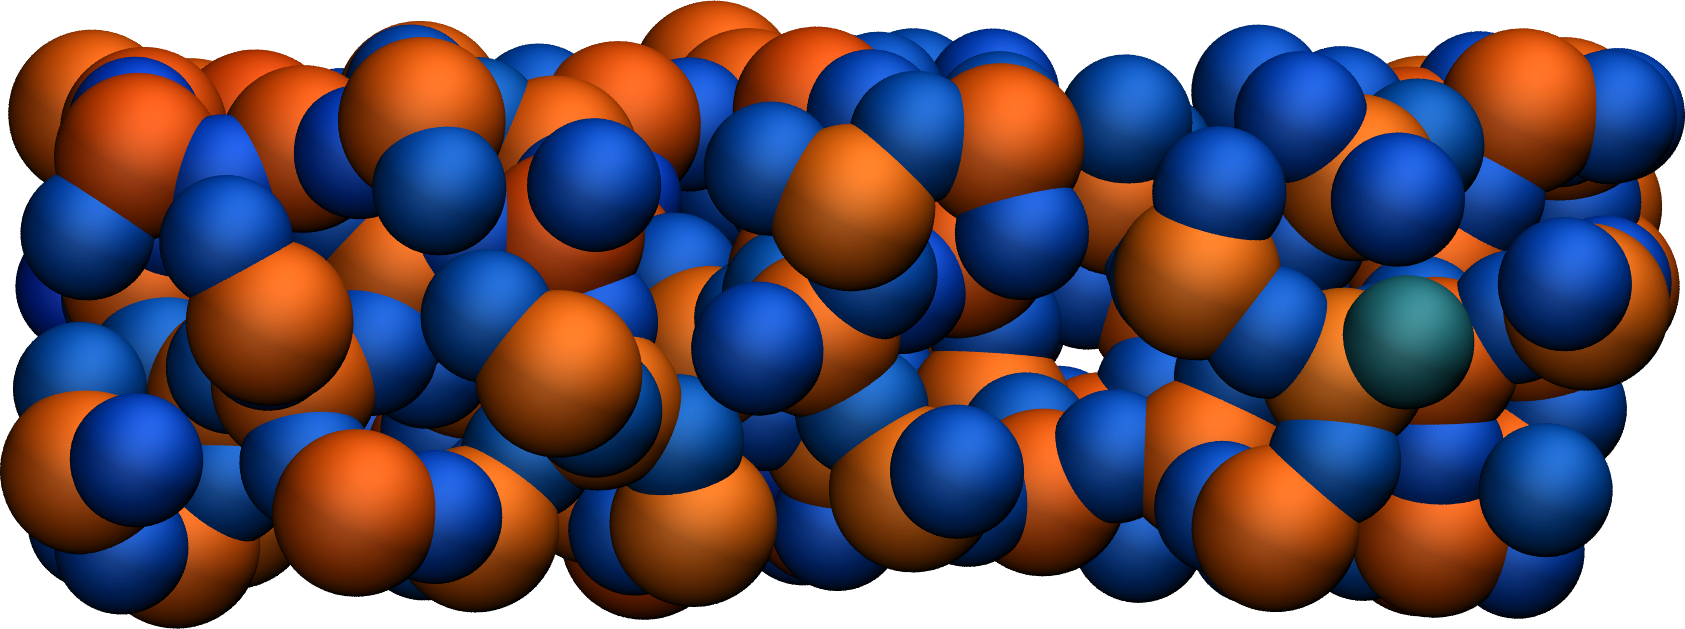
\includegraphics[width=\linewidth]{SIO-slice}
\caption{A slice of the amorphous silica, where atoms are colored by their charges.
Dangling oxygen groups appear in greenish, bulk Si atoms with a charge of about
$1.8~\text{e}$  appear in red/orange, and bulk O atoms with a charge of about
$-0.9~\text{e}$ appear in blue. To color the atoms by their charge using VMD,
use \textit{Charge} as the coloring method in the representation windows, and
then tune the \textit{Color scale} in the \textit{Color control windows}.}
\label{fig:SIO-slice}
\end{figure}

\subsubsection{Deform the structure}
Let us apply a deformation to the structure to force some $\text{Si}-\text{O}$
bonds to break (and eventually re-assemble). Next to \textit{RelaxSilica/},
create a folder, call it \textit{Deform/} and create a file called \textit{input.lmp}
in it. Copy the same lines as previously in \textit{input.lmp}:
{\normalsize \begin{verbatim}
units real
atom_style full

read_data ../RelaxSilica/silica-relaxed.data

mass 1 28.0855 # Si
mass 2 15.999 # O

pair_style reaxff NULL safezone 3.0 mincap 150
pair_coeff * * ../RelaxSilica/reaxCHOFe.ff Si O
fix myqeq all qeq/reaxff 1 0.0 10.0 1.0e-6 &
    reaxff maxiter 400
\end{verbatim}}
The only differences with the previous \textit{input.lmp} file are the paths to
the \textit{.data} and \textit{.ff} files located within \textit{RelaxSilica/}.
Copy the following lines as well:
{\normalsize \begin{verbatim}
group grpSi type 1
group grpO type 2
variable qSi equal charge(grpSi)/count(grpSi)
variable qO equal charge(grpO)/count(grpO)

thermo 200
thermo_style custom step temp etotal &
    press vol v_qSi v_qO

dump mydmp all image 200 dump.*.jpg type type &
    shiny 0.1 box no 0.01 view 0 0 zoom 1.8
dump_modify mydmp backcolor white &
    acolor 1 yellow adiam 1 2.5 &
    acolor 2 red adiam 2 2

dump dmp all custom 200 dump.lammpstrj &
    id type q x y z

fix myspec all reaxff/species 5 1 5 species.log &
    element Si O
\end{verbatim}}
Then, let us use \textit{fix nvt} instead of \textit{fix npt} to apply a
thermostat but no barostat:
{\normalsize \begin{verbatim}
fix mynvt all nvt temp 300.0 300.0 100
timestep 0.5
\end{verbatim}}
Here, no barostat is used because the box volume will be imposed by the \textit{fix deform}.

\begin{figure}
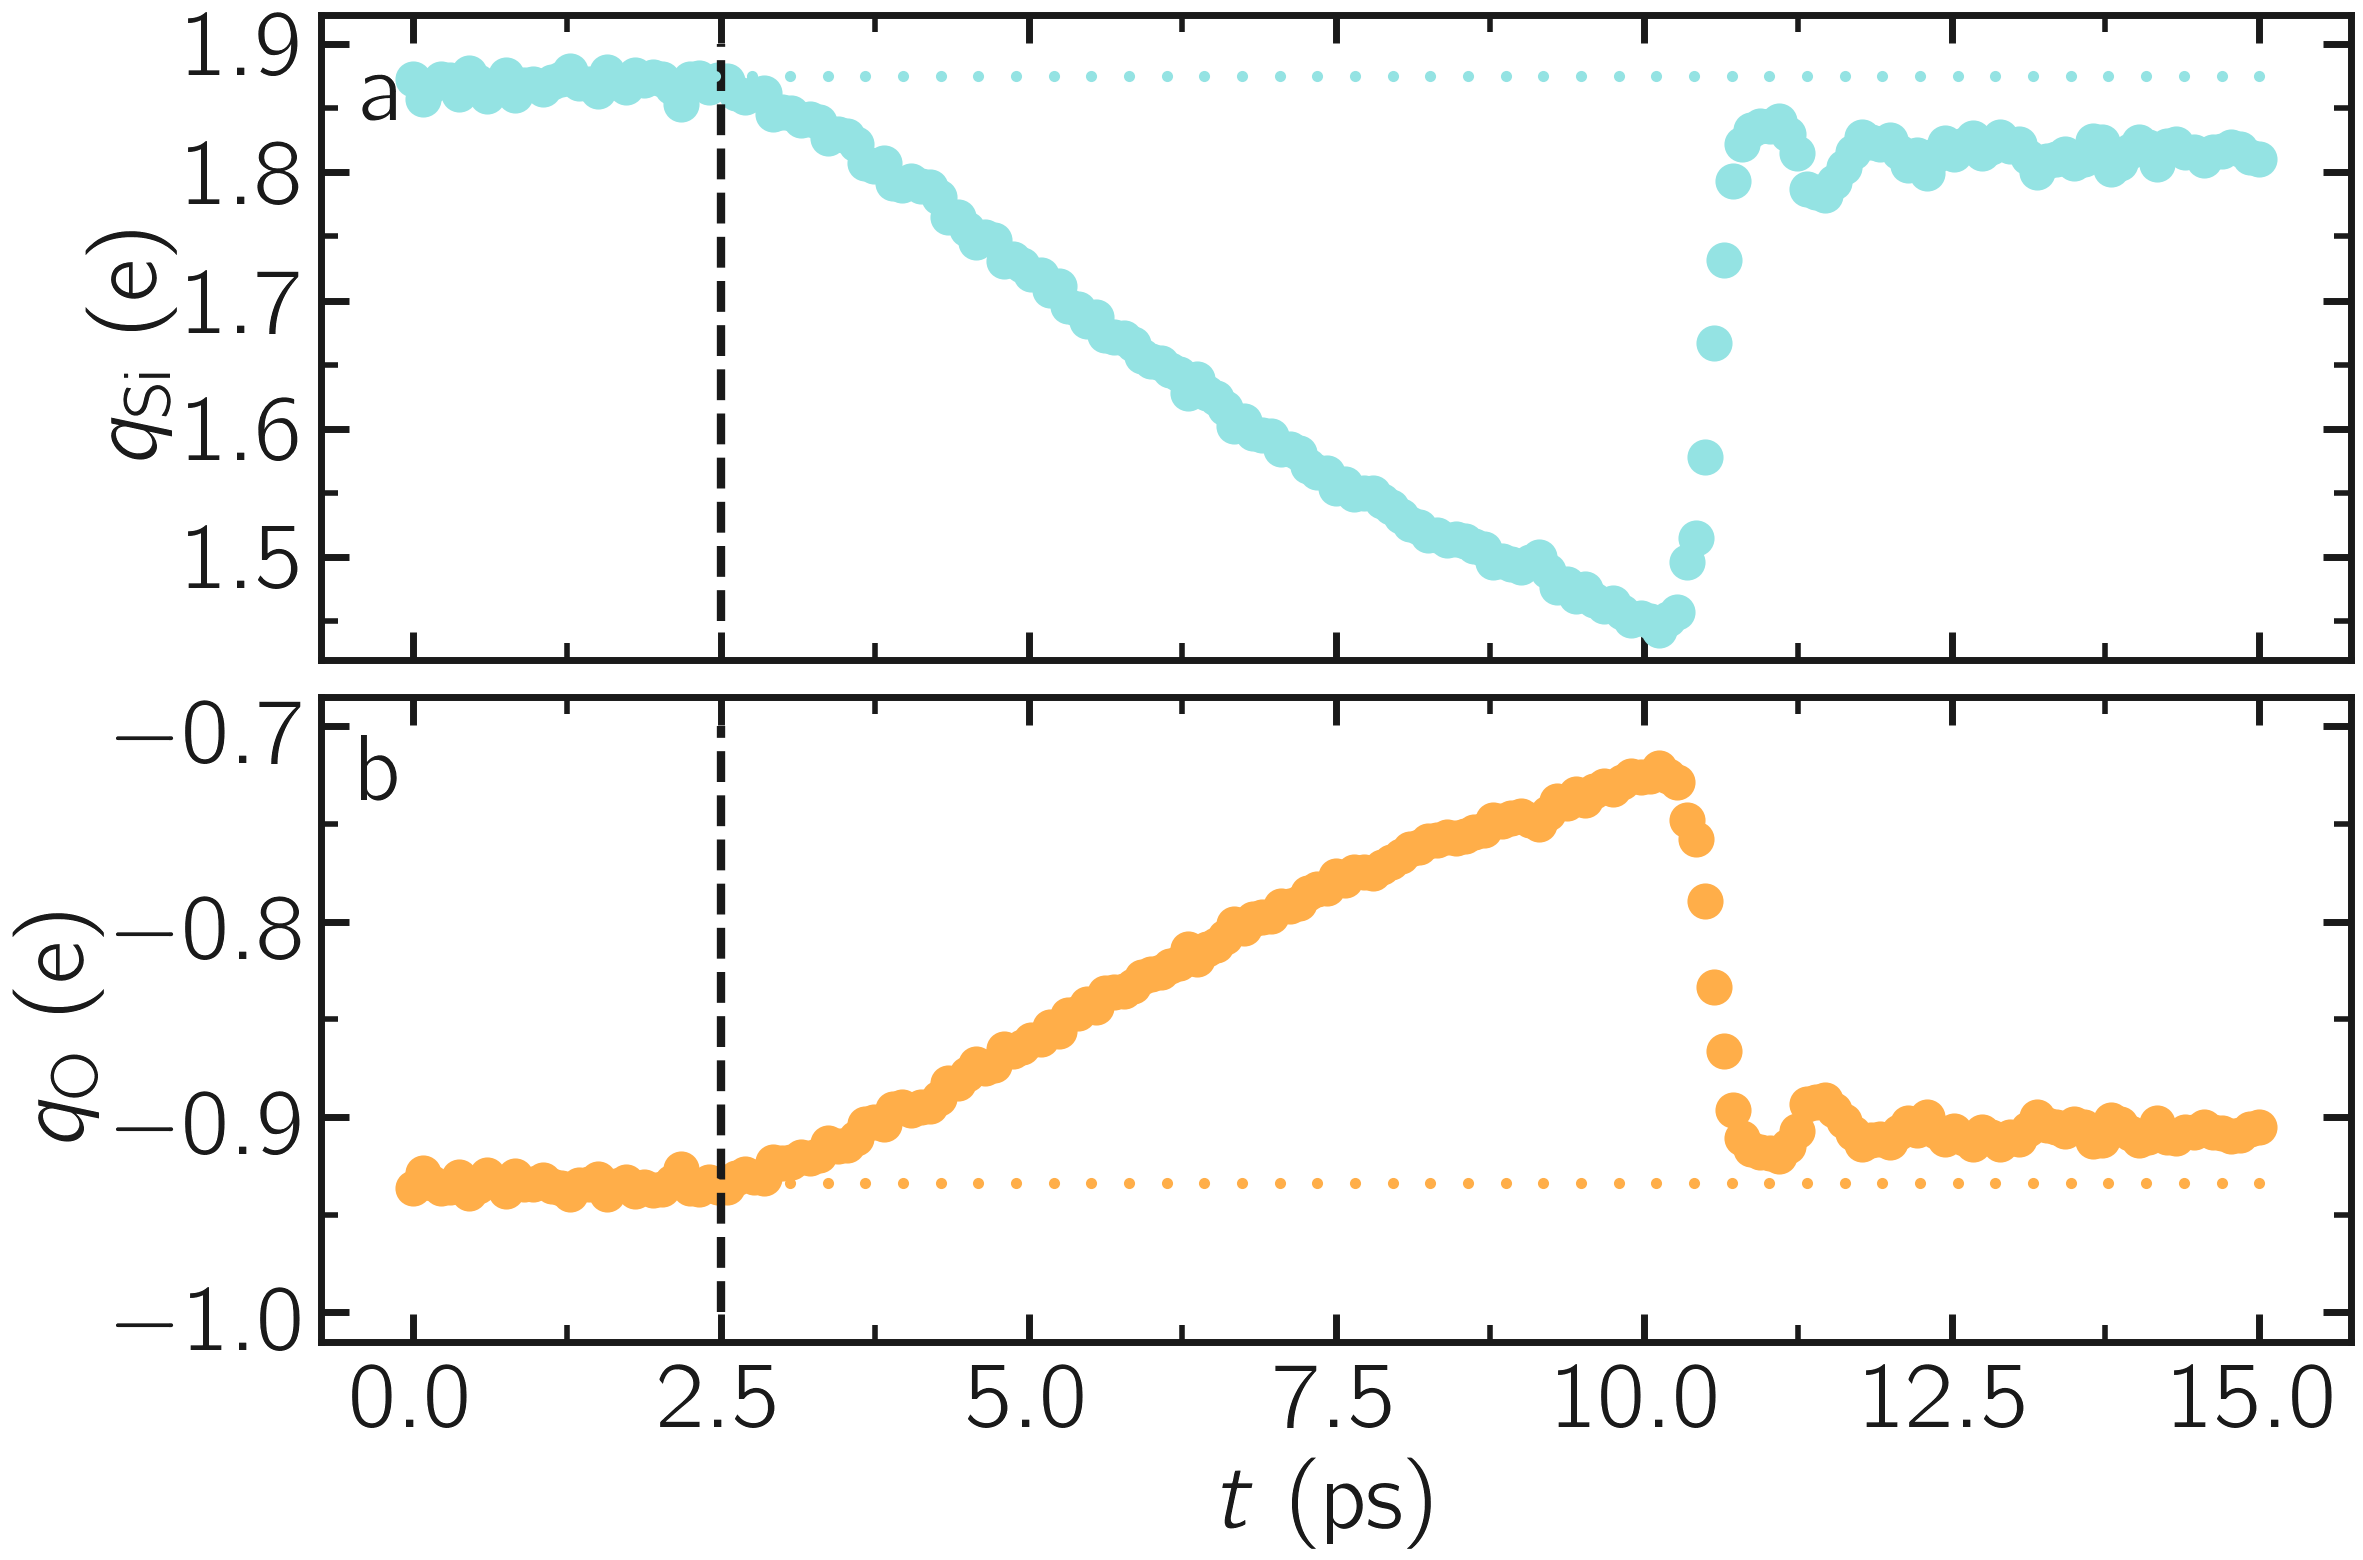
\includegraphics[width=\linewidth]{SIO-deformed-charge}
\caption{Evolution of the average charge per atom of the silicon $q_\text{Si}$
(a) and oxygen $q_\text{O}$ (b) over time $t$. The vertical dashed lines mark
the beginning of the deformation, and the horizontal dotted lines denote the
initial values for the average charge.}
\label{fig:SIO-deformed-charge}
\end{figure}

Let us run for 5000 steps without deformation, then apply the \textit{fix deform}
for elongating progressively the box along \textit{x} during 25000 steps. Add
the following line to \textit{input.lmp}:
{\normalsize \begin{verbatim}
run 5000

fix mydef all deform 1 x erate 5e-5

run 25000

write_data silica-deformed.data
\end{verbatim}}
Run the \textit{input.lmp} file using LAMMPS. During the deformation, the charge
values progressively evolve until the structure eventually breaks down. After the
structure breaks down, the charges equilibrate near new average values that differ
from the starting averages (Fig.\,\ref{fig:SIO-deformed-charge}). The difference
between the initial and the final charges can be explained by the presence of
defects as well as new solid/vacuum interfaces, and the fact that surface atoms
typically have different charges compared to bulk atoms. There is also a strong
increase in temperature during the rupture of the material (Fig.\,\ref{fig:SIO-temperature}).
At the end of the deformation, one can visualize the broken material using VMD.
Notice the different charge values of the atoms located near the vacuum interfaces,
compared to the atoms located in the bulk of the material (Fig.\,\ref{fig:SIO-deformed}).

\begin{figure}
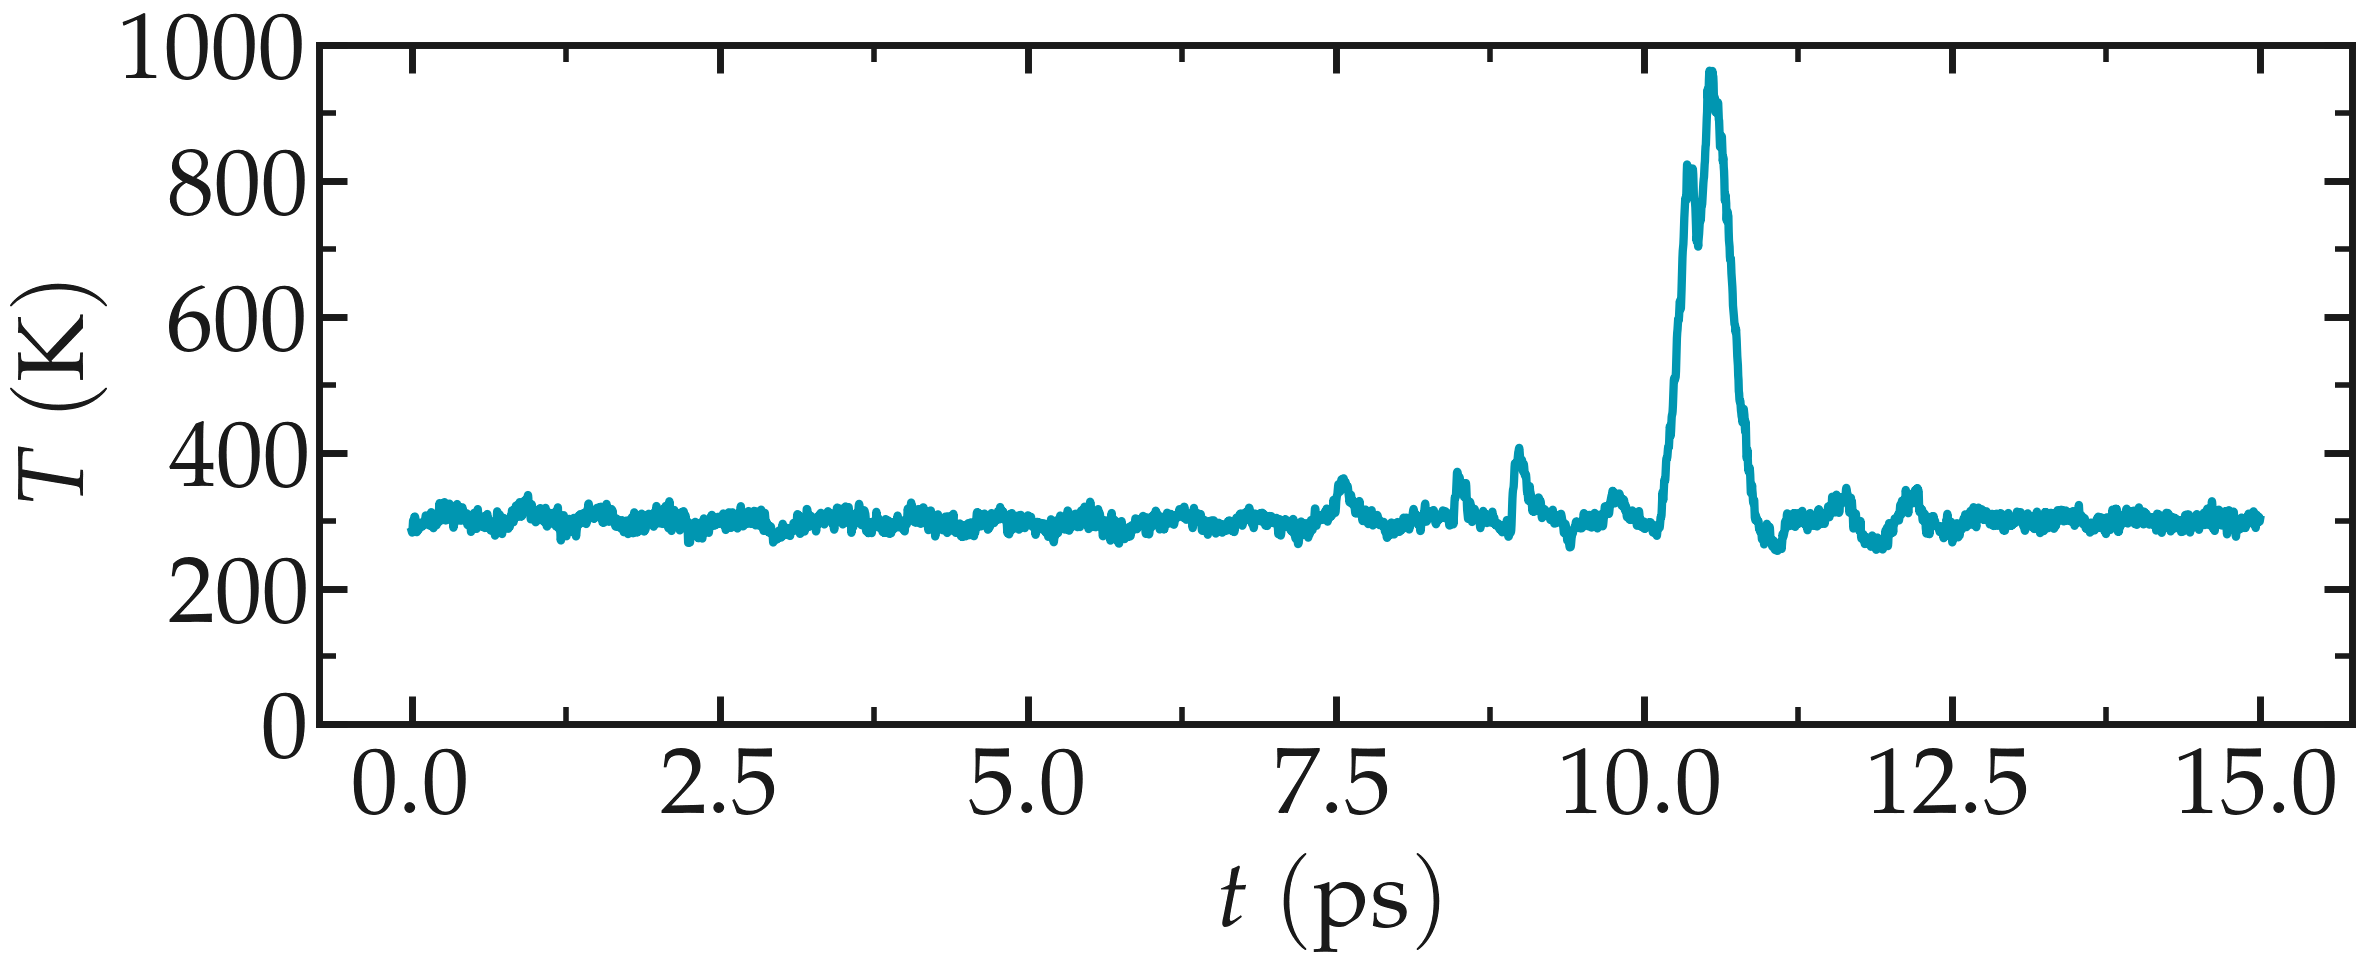
\includegraphics[width=\linewidth]{SIO-temperature}
\caption{Evolution of the temperature $T$ of the silica system over time $t$.
The material ruptures near $t = 10~\text{ps}$.}
\label{fig:SIO-temperature}
\end{figure}

\begin{figure}
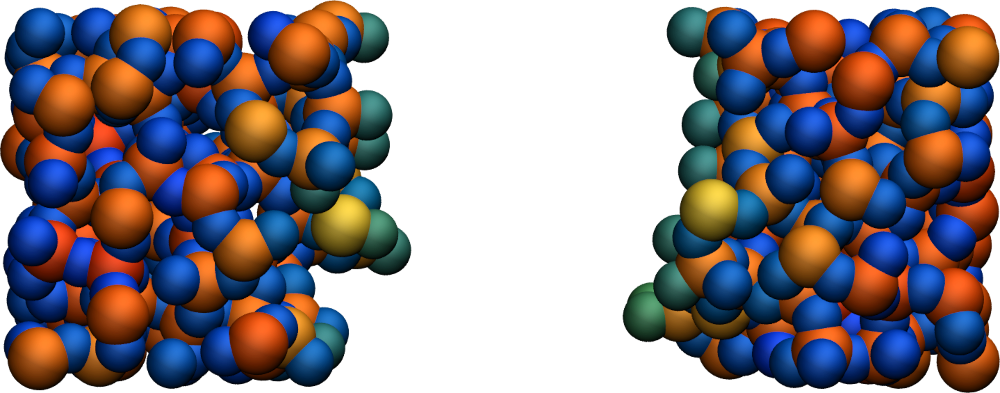
\includegraphics[width=\linewidth]{SIO-deformed}
\caption{Amorphous silicon oxide after deformation. The atoms are colored by their
charges. Dangling oxygen groups appear in greenish, bulk Si atoms with a charge of
about $1.8~\text{e}$  appear in red/orange, and bulk O atoms with a charge of
about $-0.9 ~ \text{e}$ appear in blue.}
\label{fig:SIO-deformed}
\end{figure}

One can have a look at the charge distribution after deformation, as well as during
the deformation (Fig.\,\ref{fig:SIO-distribution-bis}). As expected, the final
charge distribution slightly differs from the previously calculated. If
no new species were formed during the simulation, the \textit{species.log} file
should resemble:
{\normalsize \begin{verbatim}
#  Timestep   No_Moles   No_Specs  O384Si192
        5            1          1          1
(...)
#  Timestep   No_Moles   No_Specs  O384Si192
    30000            1          1          1
\end{verbatim}}
Sometimes, $\text{O}_2$ molecules are formed during the deformation. If this is
the case, a new column \textit{O2} appears in the \textit{species.log} file.

\begin{figure}
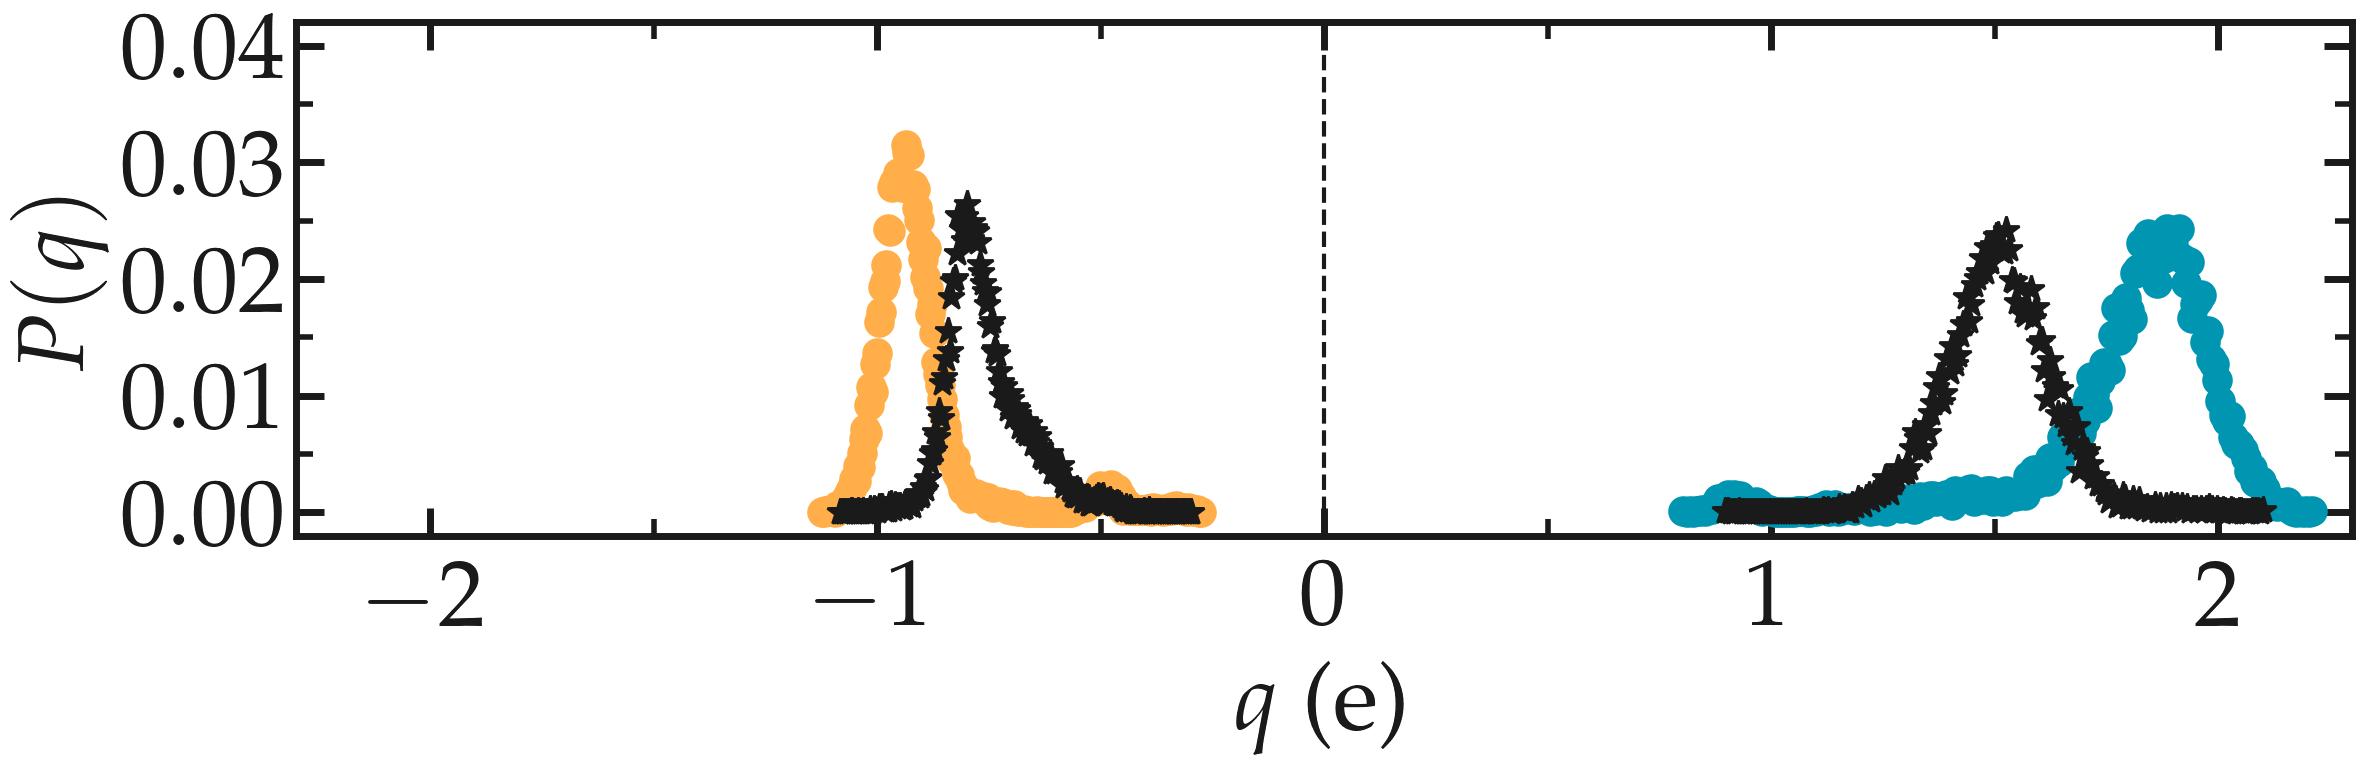
\includegraphics[width=\linewidth]{SIO-distribution-bis}
\caption{Probability distribution of charge of silicon (positive, blue) and oxygen
(negative, orange) after deformation. The stars correspond to the charge distribution
during deformation.}
\label{fig:SIO-distribution-bis}
\end{figure}

\subsubsection{Decorate the surface}
In ambient conditions, some of the surface $\text{SiO}_2$ atoms are chemically
passivated by forming covalent bonds with hydrogen (H) atom \cite{sulpizi2012silica}.
Let us add hydrogen atoms randomly to the cracked silica and observe how the
system evolves.  Next to \textit{RelaxSilica/} and \textit{Deform/}, create a folder,
and call it \textit{Decorate/}. Then, let us modify the previously generated data
file \textit{silica-deformed.data} and make space for a third atom type.
Copy \textit{silica-deformed.data} from the \textit{Deform/} folder, and modify
the first lines as follows:
{\normalsize \begin{verbatim}
576 atoms
3 atom types

(...)

Masses

1 28.0855
2 15.999
3 1.008

(...)
\end{verbatim}}
Create a file called \textit{input.lmp} into the \textit{Decorate/} folder, and
copy the following lines into it:
{\normalsize \begin{verbatim}
units real
atom_style full

read_data silica-deformed.data
displace_atoms all move -12 0 0 # optional

pair_style reaxff NULL safezone 3.0 mincap 150
pair_coeff * * ../RelaxSilica/reaxCHOFe.ff &
    Si O H
fix myqeq all qeq/reaxff 1 0.0 10.0 1.0e-6 &
    reaxff maxiter 400
\end{verbatim}}
Here, the \textit{displace\_atoms} command was used to move the center of the
crack near the center of the box. This step is optional but makes the visualization
of the interface in VMD easier. A different value for the shift may be needed in
your case, depending on the location of the crack. A difference with the previous
input is that three atom types are specified in the \textit{pair\_coeff} command,
\textit{Si O H}, instead of two.

Then, let us adapt some familiar commands to measure the charges of all three
types of atoms, and output the charge values into log files:
{\normalsize \begin{verbatim}
group grpSi type 1
group grpO type 2
group grpH type 3
variable qSi equal charge(grpSi)/count(grpSi)
variable qO equal charge(grpO)/count(grpO)
variable qH equal &
    charge(grpH)/(count(grpH)+1e-10)

thermo 5
thermo_style custom step temp etotal press &
    vol v_qSi v_qO v_qH
fix myspec all reaxff/species 5 1 5 &
    species.log element Si O H
\end{verbatim}}
Here, the $+1\text{e}-10$ was added to the denominator of the \textit{variable qH}
to avoid dividing by 0 at the beginning of the simulation. Finally, let us
create a loop with 10 steps, and create two hydrogen atoms at random locations at
every step:
{\normalsize \begin{verbatim}
fix mynvt all nvt temp 300.0 300.0 100
timestep 0.5

label loop
variable a loop 10

variable seed equal 35672+${a}
create_atoms 3 random 2 ${seed} NULL &
    overlap 2.6 maxtry 50
group grpH type 3

run 2000
write_dump all custom dump.${a}.lammpstrj &
    id type q x y z
undump mydmp

next a
jump SELF loop

write_data decorated.data
\end{verbatim}}
Here, a different \textit{lammpstrj} file is created for each step of the loop
to avoid creating dump files with varying numbers of atoms, which VMD can't read.
Once the simulation is over, it can be seen from the \textit{species.log} file that
all the created hydrogen atoms reacted with the $\text{SiO}_{2}$ structure to
form surface groups (such as hydroxyl (-OH) groups).
{\normalsize \begin{verbatim}
(...)
# Timestep   No_Moles No_Specs H20O384Si192
  20000      1        1        1
\end{verbatim}}
At the end of the simulation, hydroxyl (-OH) groups can be seen at the interfaces
(Fig.\,\ref{fig:SIO-decorated}).

\begin{figure}
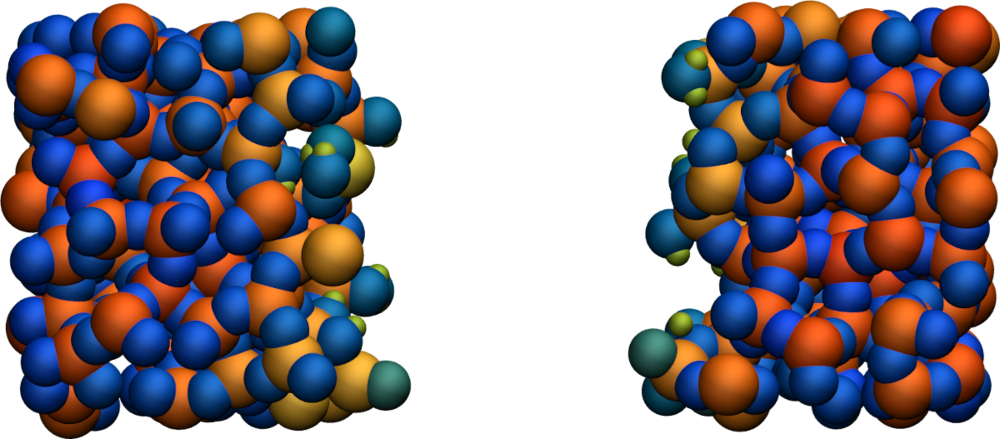
\includegraphics[width=\linewidth]{SIO-decorated}
\caption{Cracked silicon oxide after the addition of hydrogen atoms. The atoms
are colored by their charges. Dangling oxygen groups appear in greenish, bulk
Si atoms with a charge of about $1.8~\text{e}$  appear in red/orange, and bulk
O atoms with a charge of about $-0.9 ~ \text{e}$ appear in blue.}
\label{fig:SIO-decorated}
\end{figure}

\subsection{Tutorial 6: Water adsorption in silica}
\label{gcmc-silica-label}

\begin{figure}
\centering
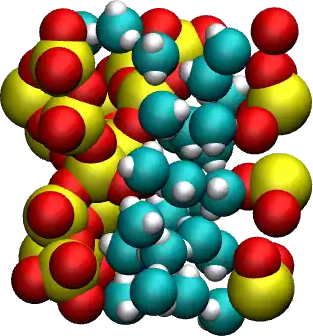
\includegraphics[width=0.55\linewidth]{GCMC}
\caption{Water molecules adsorbed in cracked silica (SiO$_2$) material as simulated
during \hyperref[gcmc-silica-label]{Tutorial 6}. Water molecules are colored in
cyan and white, oxygen (O) atoms from SiO$_2$ in red, and silicon (Si) atoms in yellow.}
\label{fig:GCMC}
\end{figure}

\noindent The objective of this tutorial is to combine molecular dynamics and
grand canonical Monte Carlo simulations to compute the adsorption of water
molecules in cracked silica material (Fig.\,\ref{fig:GCMC}). This tutorial
illustrates the use of the grand canonical ensemble in molecular simulation, an
open ensemble in which the number of atoms or molecules within the simulation
box is not constant. When using the grand canonical ensemble, it is possible to
impose the chemical potential (or pressure) of a given fluid in a nanoporous structure.

\subsubsection{Generation of the silica block}
\noindent Let us first generate a block of amorphous silica ($\text{SiO}_2$).
To do so, we are going to replicate a building block containing 3 Si and 6 O atoms.
Create two folders side by side, and name them respectively \textit{Potential/}
and \textit{SilicaBlock/}. The initial data file for the SiO atoms called
\href{https://raw.githubusercontent.com/lammpstutorials/lammpstutorials-article/main/files/tutorial6/SiO.data}{\textit{SiO.data}}
must be downloaded and saved in \textit{SilicaBlock/}. This data file contains
the coordinates of the 9 atoms, their masses, and their charges.

Let us replicate these atoms using LAMMPS, and apply an annealing procedure to
obtain a block of amorphous silica. Create a new input file called \textit{input.lmp}
in the \textit{SilicaBlock/} folder, and copy
the following lines into it:
{\normalsize \begin{verbatim}
units metal
boundary p p p
atom_style full
pair_style vashishta
neighbor 1.0 bin
neigh_modify delay 1
\end{verbatim}}
The main difference from some of the previous tutorials is the use of the \textit{Vashishta}
pair style. The Vashishta potential is a bond-angle energy-based potential, it deduces
the bonds between atoms from their relative positions \cite{vashishta1990interaction}.

Let us then import the system consisting of 9 atoms, and replicate it four times
in all three directions of space, thus creating a system with 576 atoms. Add the
following lines into \textit{input.lmp}:
{\normalsize \begin{verbatim}
read_data SiO.data
replicate 4 4 4
\end{verbatim}}
Then, let us specify the pair coefficients by indicating that the first atom type
is \textit{Si} and the second is \textit{O}. Let us also add a dump command to
print out the positions of the atoms every 5000 steps:
{\normalsize \begin{verbatim}
pair_coeff * * &
    ../Potential/SiO.1990.vashishta Si O
\end{verbatim}}
Download the \href{https://raw.githubusercontent.com/lammpstutorials/lammpstutorials-article/main/files/tutorial6/SiO.1990.vashishta}{SiO.1990.vashishta},
and copy it within the \textit{Potential/} folder.

Let us add a \textit{dump image} command to \textit{input.lmp} to follow the
evolution of the system with time:
{\normalsize \begin{verbatim}
dump mydmp all image 200 dump.*.jpg type type &
    shiny 0.1 box no 0.01 view 0 0 zoom 1.2
dump_modify mydmp backcolor white &
    acolor 1 yellow adiam 1 2.5 &
    acolor 2 red adiam 2 2
thermo 1000
thermo_style custom step temp etotal &
    vol lx ly lz
\end{verbatim}}
Thanks to the \textit{thermo\_style custom} command, the box size along each direction
will be printed in the log file.

Finally, let us create the last part of our script. The annealing procedure is
made of four consecutive runs. First, a $50\,\text{ps}$ phase at $T = 6000\,\text{K}$
and isotropic pressure coupling with desired pressure $p = 100\,\text{atm}$:
{\normalsize \begin{verbatim}
velocity all create 6000 4928459 &
    rot yes dist gaussian
fix npt1 all npt temp 6000 6000 0.1 &
    iso 100 100 1
timestep 0.001
run 50000
\end{verbatim}}
Then, a second phase during which the system is cooled down from $T = 6000\,\text{K}$
to $T = 4000\,\text{K}$. An anisotropic pressure coupling is used, allowing all
three dimensions of the box to evolve independently from one another:
{\normalsize \begin{verbatim}
fix npt1 all npt temp 6000 4000 0.1 &
    aniso 100 100 1
run 50000
\end{verbatim}}
Then, let us cool down the system further while also reducing the pressure, and then
perform a small equilibration step at the final desired condition, $T = 300\,\text{K}$ and $p = 1\,\text{atm}$.
{\normalsize \begin{verbatim}
fix npt1 all npt temp 4000 300 0.1 &
    aniso 100 1 1
run 200000
fix npt1 all npt temp 300 300 0.1 &
    aniso 1 1 1
run 50000
write_data amorphousSiO.data
\end{verbatim}}
Here, an isotropic barostat is used for the melted phase at $T = 6000\,\text{K}$,
and an anisotropic barostat is used for all following phases. With the anisotropic
barostat, all three directions of space are adjusted independently from one another.
An anisotropic barostat is usually a better choice for a solid phase. For a liquid
or a gas, an isotropic barostat is usually the best choice.

Run the simulation using LAMMPS. From the \textit{Charts} window, the temperature
can be seen to follow well the desired annealing procedure (Fig.\,\ref{fig:GCMC-temperature}).
The evolution of the box dimensions over time confirms that the box was indeed
deformed isotropically during the first stage of the simulation, and then anisotropically
(Fig.\,\ref{fig:GCMC-dimension}). After running
the simulation, the final LAMMPS topology file called \textit{amorphousSiO.data}
will be located in \textit{SilicaBlock/} (Fig.\,\ref{fig:GCMC-snapshot}).

\begin{figure}
\centering
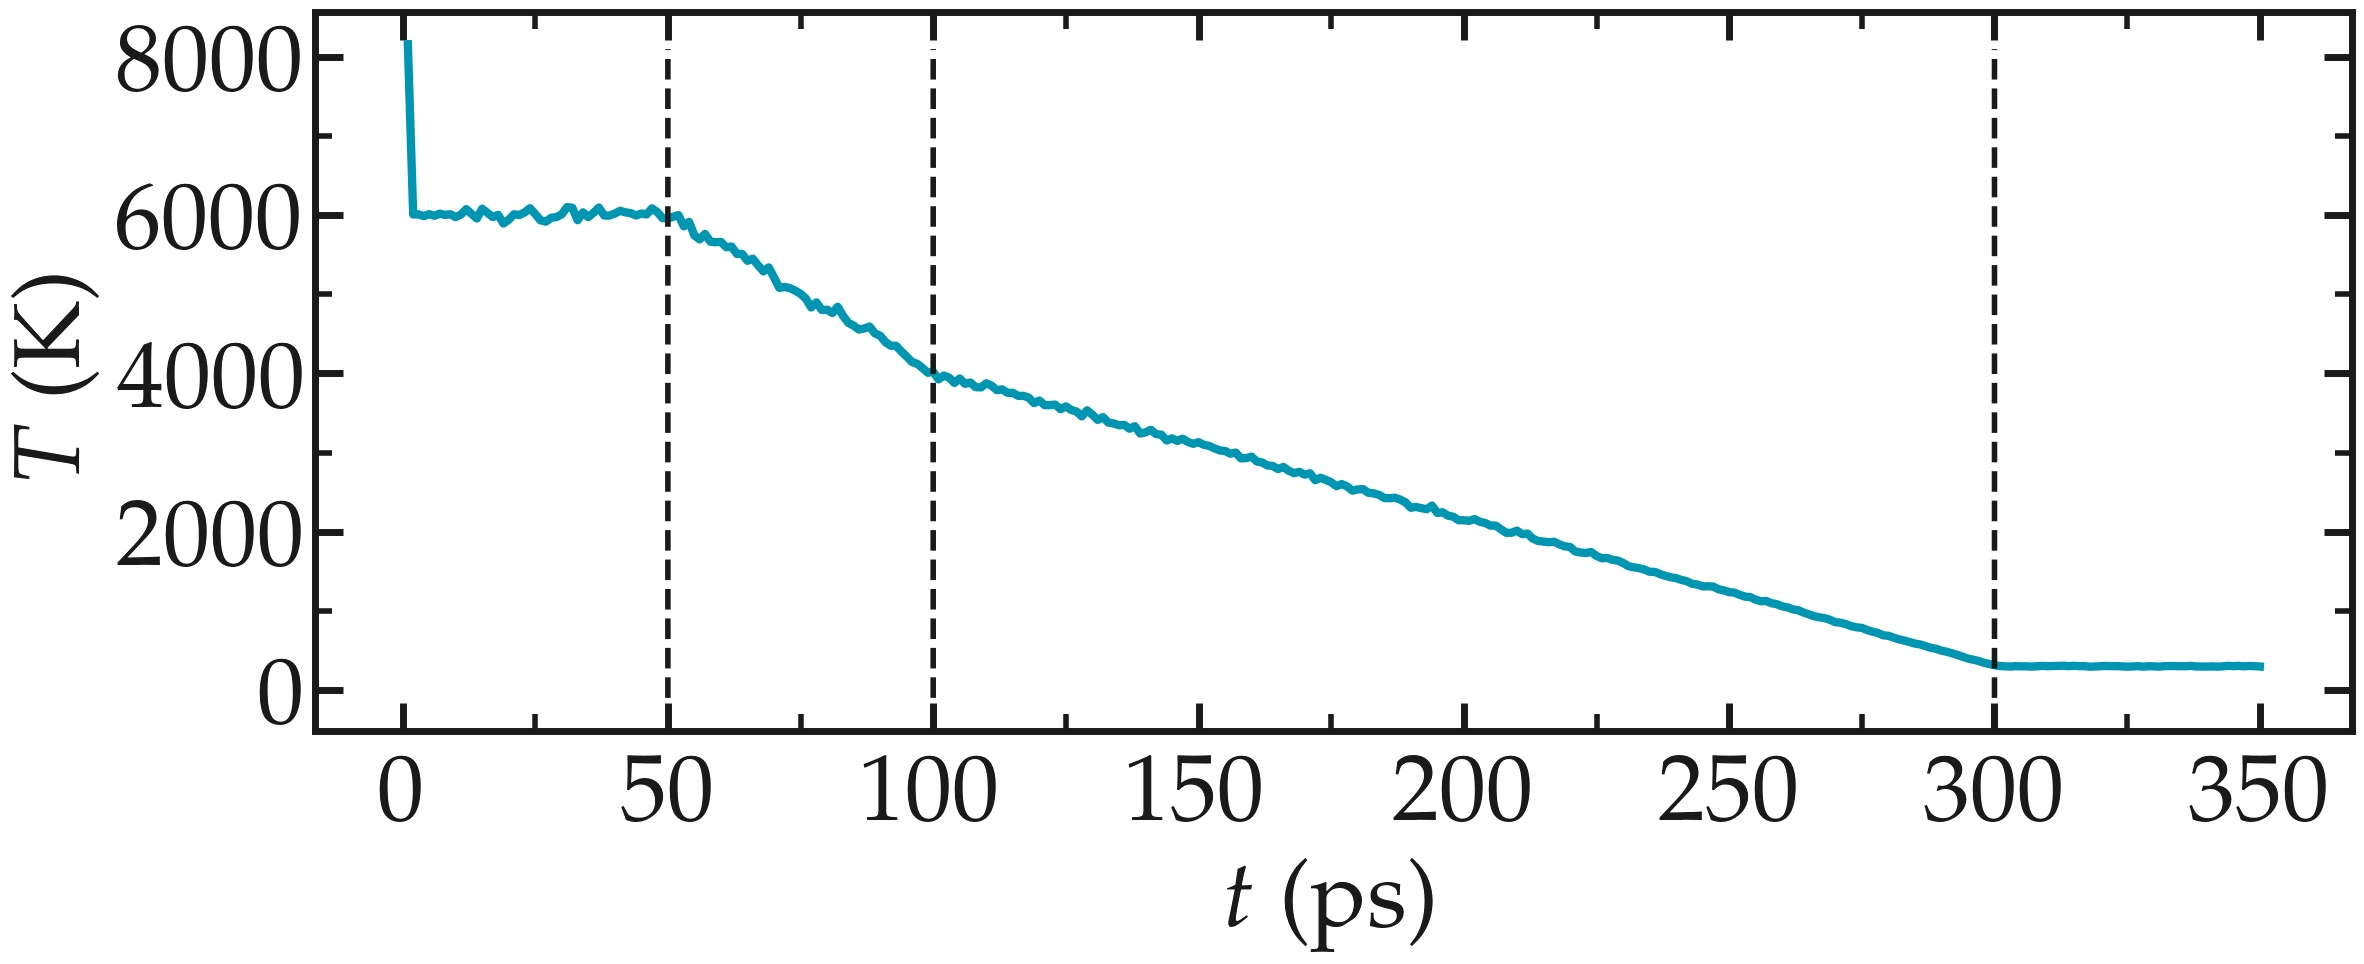
\includegraphics[width=\linewidth]{GCMC-temperature}
\caption{Temperature $T$ of the system during annealing. The vertical dashed lines
mark the transition between the different phases of the simulation.}
\label{fig:GCMC-temperature}
\end{figure}

\begin{figure}
\centering
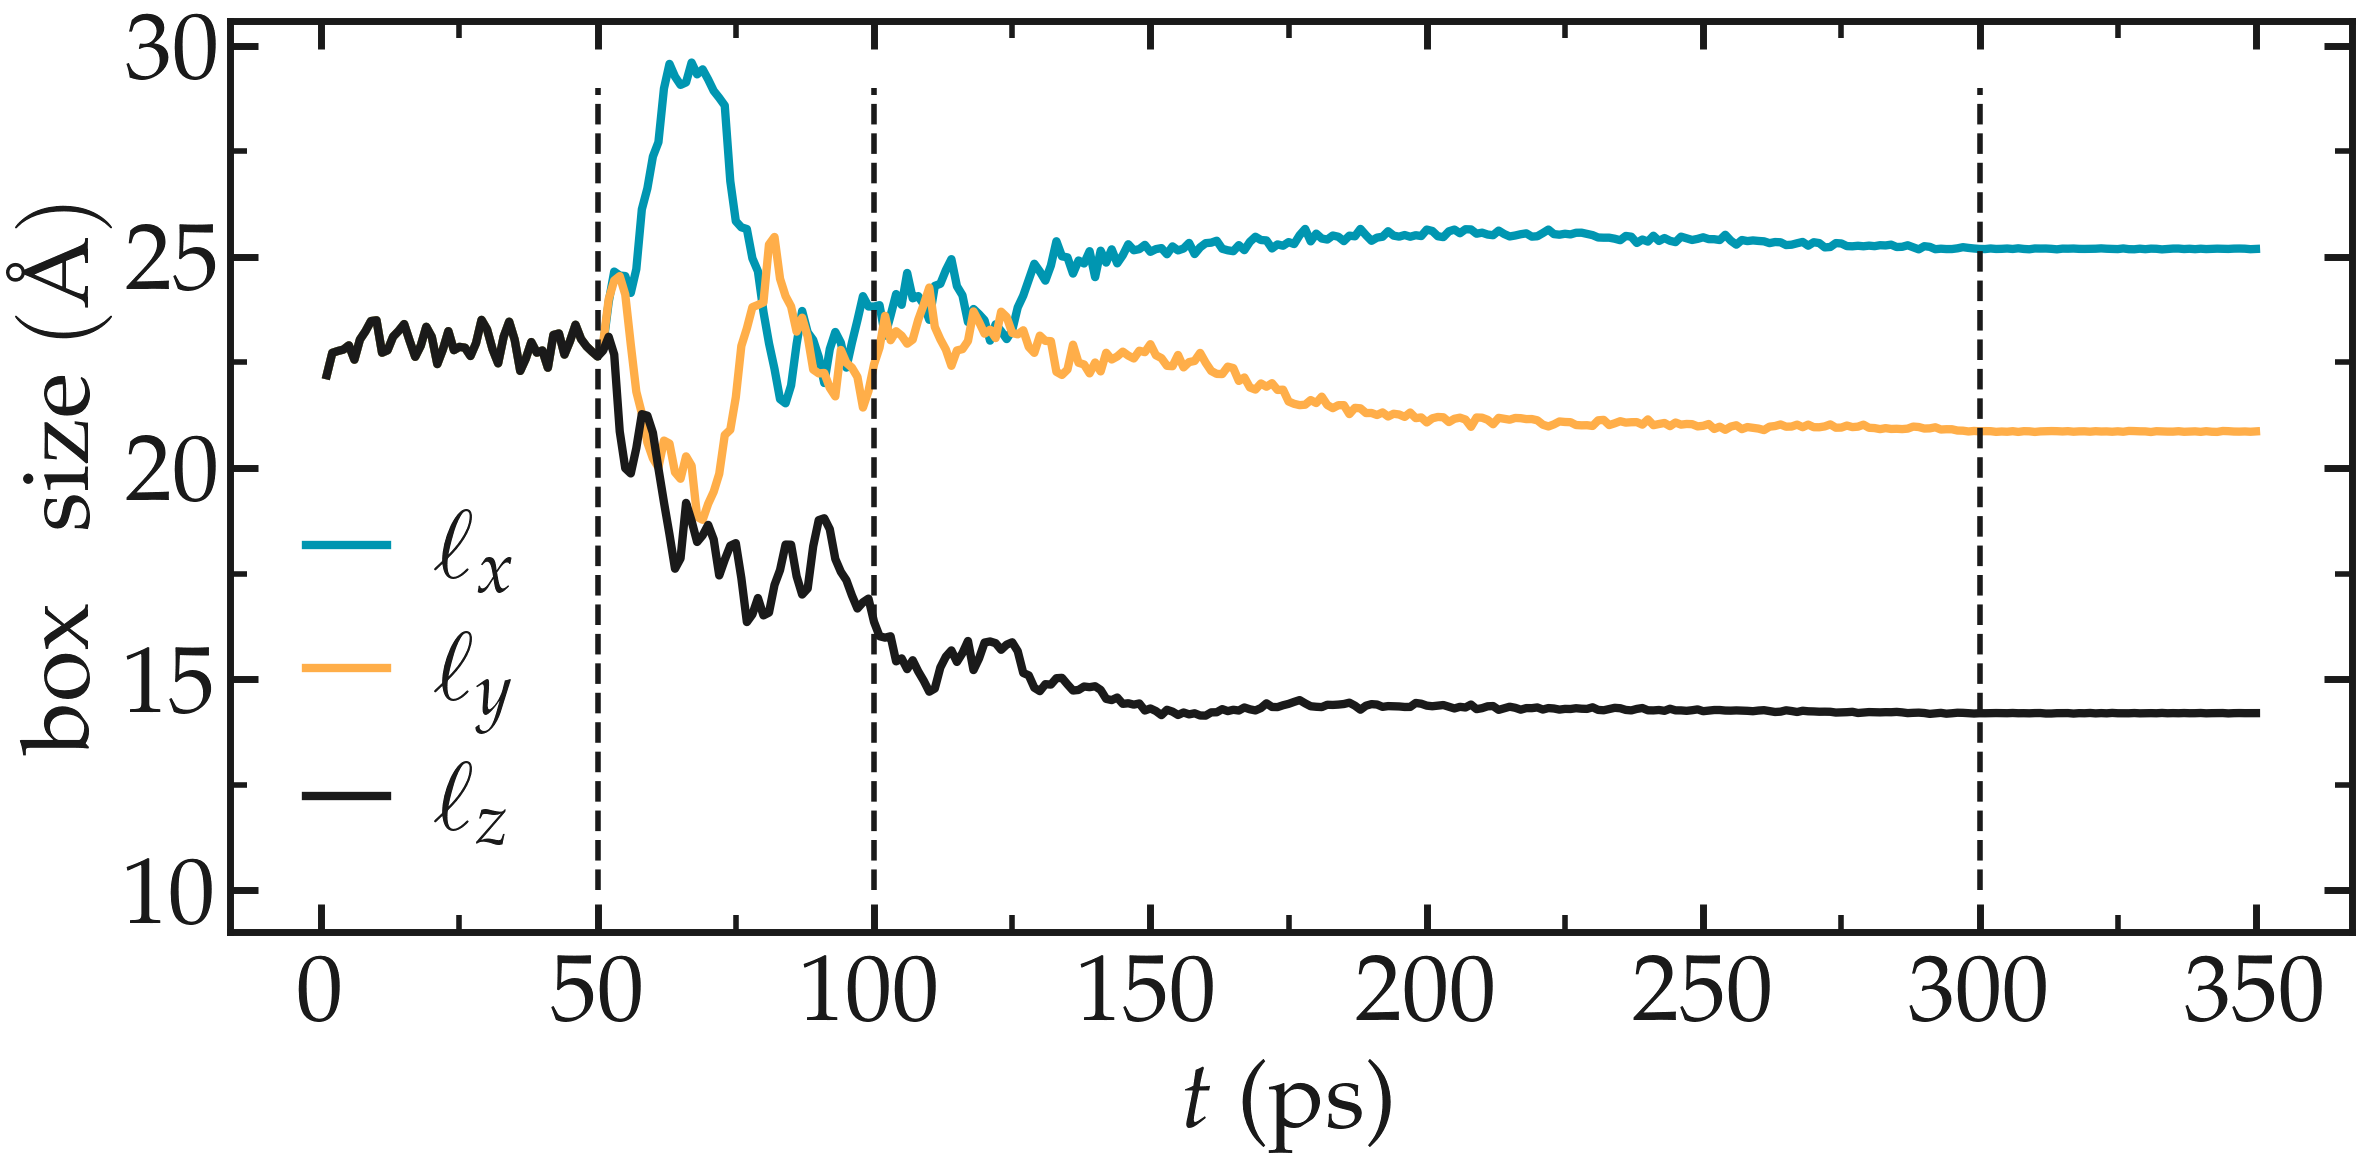
\includegraphics[width=\linewidth]{GCMC-dimension}
\caption{Box dimensions along $x$ (blue), $y$ (orange), and $z$ (dark) during
annealing. The vertical dashed lines mark the transition between the different
phases of the simulation.}
\label{fig:GCMC-dimension}
\end{figure}

\begin{figure}
\centering
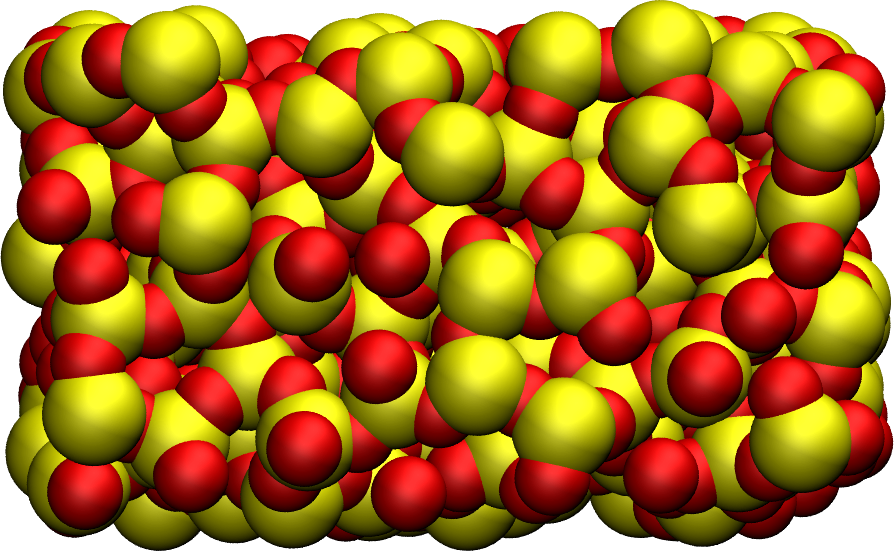
\includegraphics[width=0.9\linewidth]{GCMC-snapshot}
\caption{Final amorphous silica ($\text{SiO}_2$). The silicon atoms are
represented in yellow, and the oxygen atoms in red.}
\label{fig:GCMC-snapshot}
\end{figure}

\subsubsection{Cracking the silica}
Let us dilate the block of silica until a crack forms. Create a new folder
called \textit{Cracking/} next to \textit{SilicaBlock/}, as well as a new
\textit{input.lmp} file starting with familiar lines as previously:
{\normalsize \begin{verbatim}
units metal
boundary p p p
atom_style full
neighbor 1.0 bin
neigh_modify delay 1

read_data ../SilicaBlock/amorphousSiO.data

pair_style vashishta
pair_coeff * * &
    ../Potential/SiO.1990.vashishta Si O
dump dmp all atom 1000 dump.lammpstrj
\end{verbatim}}
Let us progressively increase the size of the box in the $x$ direction, thus forcing
the silica to deform and eventually crack. To do so, a loop based on the jump command
is used. At every step of the loop, the box dimension over $x$ will be multiplied
by a scaling factor 1.005. Add the following lines into the \textit{input.lmp}:
{\normalsize \begin{verbatim}
fix nvt1 all nvt temp 300 300 0.1
timestep 0.001
thermo 1000
variable var loop 45
label loop
change_box all x scale 1.005 remap
run 2000
next var
jump input.lmp loop
run 20000
write_data dilatedSiO.data
\end{verbatim}}
The \textit{fix nvt} is used to control the temperature of the system, while the
\textit{change\_box} command imposes incremental deformations of the box. Different
scaling factors or different numbers of steps can be used to generate different
defects in the silica. After the expansion, a final equilibration step of a duration
of 20 picoseconds is performed. If you look at the \textit{dump.lammpstrj} file
using VMD, you can see the expansion occurring step-by-step, and the atoms
progressively adjusting to the box dimensions. At first, the deformations are
reversible (elastic regime). At some point, bonds start breaking and dislocations
appear (plastic regime). The final system is shown in Fig.\,\ref{fig:GCMC-cracked}.

\begin{figure}
\centering
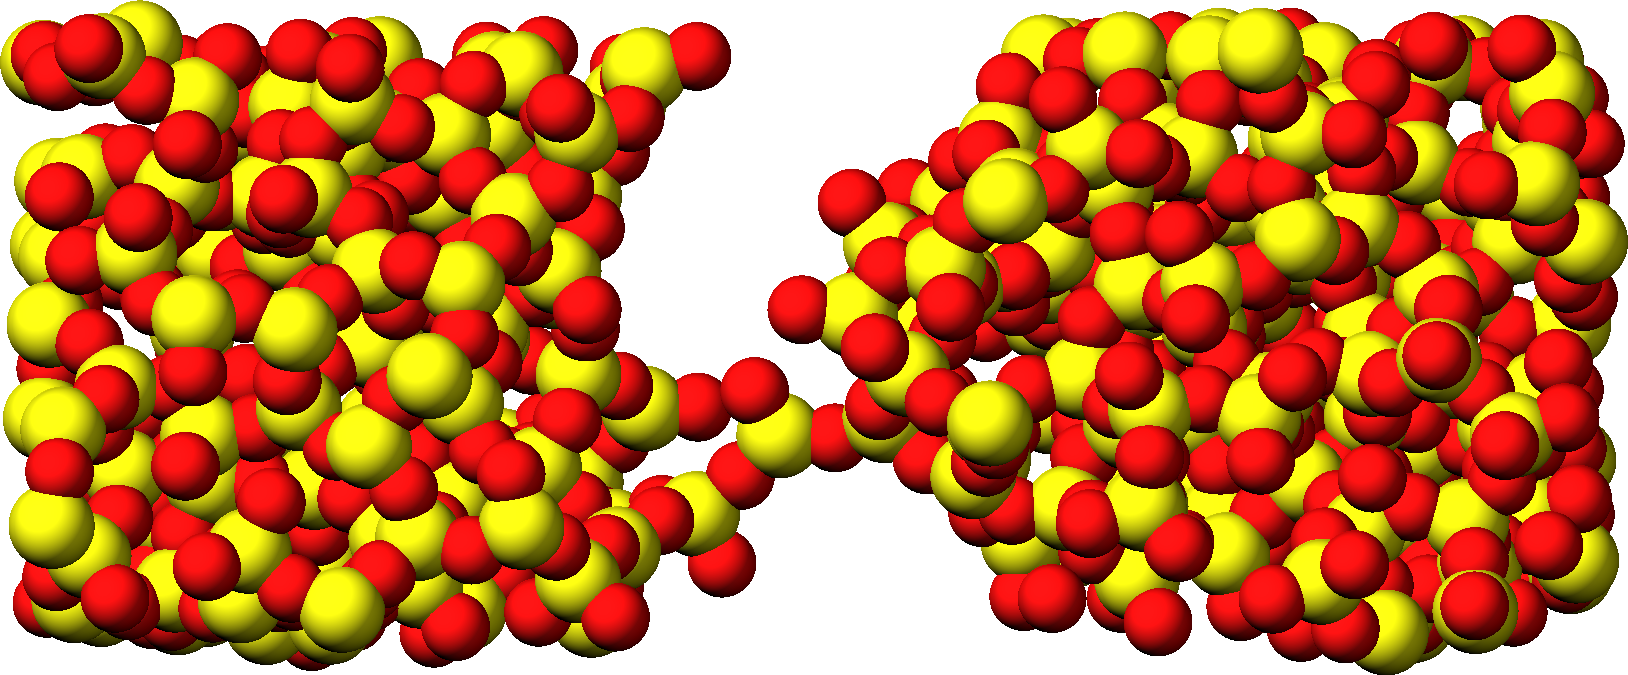
\includegraphics[width=\linewidth]{GCMC-cracked}
\caption{Block of silica after deformation. The silicon atoms are represented in
yellow, and the oxygen atoms in red. Some holes are visible.}
\label{fig:GCMC-cracked}
\end{figure}

\subsubsection{Adding water}
\noindent In order to add the water molecules to the silica, we are going to use
the Monte Carlo method in the grand canonical ensemble (GCMC). In short, the
system is put into contact with a virtual reservoir of a given chemical potential
$\mu$, and multiple attempts to insert water molecules at random positions are
made. Each attempt is either accepted or rejected based on energy considerations.
Find more details in classical textbooks like Ref.~\citenum{frenkel2023understanding}.

\paragraph{Using hydrid potentials}
\noindent Create a new folder called \textit{Addingwater/}. Download and save
the water molecule template called
\href{https://raw.githubusercontent.com/lammpstutorials/lammpstutorials-article/main/files/tutorial6/H2O.mol}{\textit{H2O.mol}}
within the \textit{Addingwater/} folder. Create a new input file called \textit{input.lmp}
within \textit{Addingwater/}, and copy the following lines into it:
{\normalsize \begin{verbatim}
units metal
boundary p p p
atom_style full
neighbor 1.0 bin
neigh_modify delay 1
pair_style hybrid/overlay vashishta &
    lj/cut/tip4p/long 3 4 1 1 0.1546 10
kspace_style pppm/tip4p 1.0e-4
bond_style harmonic
angle_style harmonic
\end{verbatim}}
There are several differences with the previous input files used in this tutorial.
From now on, the system will combine water and silica, and therefore two force
fields are combined: Vashishta for $\text{SiO}_2$, and lj/cut/tip4p/long for
TIP4P water model (here the TIP4P/2005 model is used \cite{abascal2005general}).
Combining the two force fields is done using the \textit{hybrid/overlay} pair
style. The PPPM solver \cite{luty1996calculating} is set with the \textit{kspace}
command, and is used to calculate the long-range Coulomb interactions associated
with \textit{tip4p/long}. Finally, the style for the bonds
and angles of the water molecules are defined, although they are not important
since TIP4P/2005 is a rigid water model.

Before going further, we also need to make a few changes to our data file.
Currently, \textit{dilatedSiO.data} only includes two atom types, but we need four.
Copy the previously generated \textit{dilatedSiO.data} file within \textit{Addingwater/}.
Currently, \textit{dilatedSiO.data} starts with:
{\normalsize \begin{verbatim}
576 atoms
2 atom types

-3.517115256285223 24.10269296788487 xlo xhi
0.5721674106566077 20.013410300943264 ylo yhi
1.3237302567479095 19.261847454851658 zlo zhi

Masses

1 28.0855
2 15.9994

Atoms # full

(...)
\end{verbatim}}
Make the following changes to allow for the addition of water molecules. Modify
the file so that it looks like the following (with 4 atom types, 1 bond type,
1 angle type, and four masses):
{\normalsize \begin{verbatim}
576 atoms
4 atom types
1 bond types
1 angle types

2 extra bond per atom
1 extra angle per atom
2 extra special per atom

-3.517115256285223 24.10269296788487 xlo xhi
0.5721674106566077 20.013410300943264 ylo yhi
1.3237302567479095 19.261847454851658 zlo zhi

Masses

1 28.0855
2 15.9994
3 15.9994
4 1.008

Atoms # full

(...)
\end{verbatim}}
Doing so, we anticipate that there will be 4 atom types in the simulations,
with O and H of $\text{H}_2\text{O}$ having indexes 3 and 4, respectively. There
will also be 1 bond type and 1 angle type. The extra bond, extra angle, and
extra special lines are here for memory allocation. We can continue to fill in
the \textit{input.lmp} file, by adding the system definition:
{\normalsize \begin{verbatim}
read_data dilatedSiO.data
molecule h2omol H2O.mol
lattice sc 3
create_atoms 0 box mol h2omol 45585
lattice none 1

group SiO type 1 2
group H2O type 3 4
\end{verbatim}}
After reading the data file and defining the h2omol molecule from the \textit{H2O.txt}
file, the \textit{create\_atoms} command is used to include some water molecules
in the system on a simple cubic lattice. Not adding a molecule before starting
the GCMC steps usually leads to failure. Note that here, most water molecules
overlap with the silica. These overlapping water molecules will have to be
deleted before starting the simulation (see below). Then, add the following
settings to \textit{input.lmp}:
{\normalsize \begin{verbatim}
pair_coeff * * vashishta &
    ../Potential/SiO.1990.vashishta &
    Si O NULL NULL
pair_coeff * * lj/cut/tip4p/long 0 0
pair_coeff 1 3 lj/cut/tip4p/long 0.0057 4.42
pair_coeff 2 3 lj/cut/tip4p/long 0.0043 3.12
pair_coeff 3 3 lj/cut/tip4p/long 0.008 3.1589
pair_coeff 4 4 lj/cut/tip4p/long 0.0 0.0
bond_coeff 1 0 0.9572
angle_coeff 1 0 104.52
\end{verbatim}}
The force field Vashishta applies only to Si (type 1) and O of $\text{SiO}_2$ (type 2),
and not to the O and H of $\text{H}_2\text{O}$, thanks to the NULL parameters
used for atoms of types 3 and 4. Pair coefficients for the lj/cut/tip4p/long
potential are defined between O($\text{H}_2\text{O}$) and between H($\text{H}_2\text{O}$)
atoms, as well as between O($\text{SiO}_2$)-O($\text{H}_2\text{O}$) and
Si($\text{SiO}_2$)-O($\text{H}_2\text{O}$). Therefore, the fluid-fluid and the
fluid-solid interactions will be dealt with by the lj/cut/tip4p/long potential.

Add the following lines as well:
{\normalsize \begin{verbatim}
variable oxygen atom "type==3"
group oxygen dynamic all var oxygen
variable nO equal count(oxygen)
thermo_style custom step temp etotal v_nO
thermo 1000

fix shak H2O shake 1.0e-4 200 0 b 1 a 1 &
    mol h2omol
\end{verbatim}}
The number of oxygen atoms from water molecules (i.e. the number of molecules)
is calculated by the \textit{nO} variable, and will be printed in the log file.
The SHAKE algorithm is used to maintain the shape of the water molecules over time,
as seen in \hyperref[sheared-confined-label]{tutorial 4}.

Finally, let us delete the overlapping water molecules, and create images
of the system using \textit{dump image}:
{\normalsize \begin{verbatim}
delete_atoms overlap 2 H2O SiO mol yes

dump mydmp all image 1000 dump.*.jpg type type &
    shiny 0.1 box yes 0.01 view 0 0 zoom 1.2
dump_modify mydmp backcolor white &
    acolor 1 yellow adiam 1 2.5 &
    acolor 2 red adiam 2 2 &
    acolor 3 cyan adiam 3 2 &
    acolor 4 white adiam 4 1 &
    boxcolor black
\end{verbatim}}

\paragraph{GCMC simulation}
To prepare for the GCMC simulation, let us make the first equilibration step by
adding the following lines into \textit{input.lmp}:
{\normalsize \begin{verbatim}
compute_modify thermo_temp dynamic yes
compute ctH2O H2O temp
compute_modify ctH2O dynamic yes
fix mynvt1 H2O nvt temp 300 300 0.1
fix_modify mynvt1 temp ctH2O
compute ctSiO SiO temp
fix mynvt2 SiO nvt temp 300 300 0.1
fix_modify mynvt2 temp ctSiO
timestep 0.001

run 5000
\end{verbatim}}
Two different thermostats are used for $\text{SiO}_2$ and $\text{H}_2\text{O}$,
respectively. Using separate thermostats is usually better when the system contains
two separate species, such as a solid and a liquid. It is particularly important
to use two thermostats here because the number of water molecules will fluctuate
with time. The \textit{compute\_modify} with \textit{dynamic yes} for water is
used to specify that the number of molecules is not constant.

Finally, let us use the \textit{fix gcmc} and perform the grand canonical Monte
Carlo steps. Add the following lines into \textit{input.lmp}:
{\normalsize \begin{verbatim}
variable tfac equal 5.0/3.0
fix fgcmc H2O gcmc 100 100 0 0 65899 300 &
    -0.5 0.1 mol h2omol tfac_insert ${tfac} &
    group H2O shake shak full_energy &
    pressure 10000
run 45000
\end{verbatim}}
The \textit{tfac\_insert} option ensures the correct estimate for the temperature
of the inserted water molecules by taking into account the internal degrees of
freedom. Running this simulation, you should see the number of molecules increasing
progressively. When using the pressure argument, LAMMPS ignores the value of the
chemical potential (here $\mu = -0.5\,\text{eV}$, which corresponds roughly to
ambient conditions, i.e. to a relative humidity $\text{RH} \approx 50\,\%$ \cite{gravelle2020multi}.)
The large pressure value of 10000 bars was chosen to ensure that some successful
insertions of molecules would occur during the extremely short duration of this simulation.

\begin{figure}
\centering
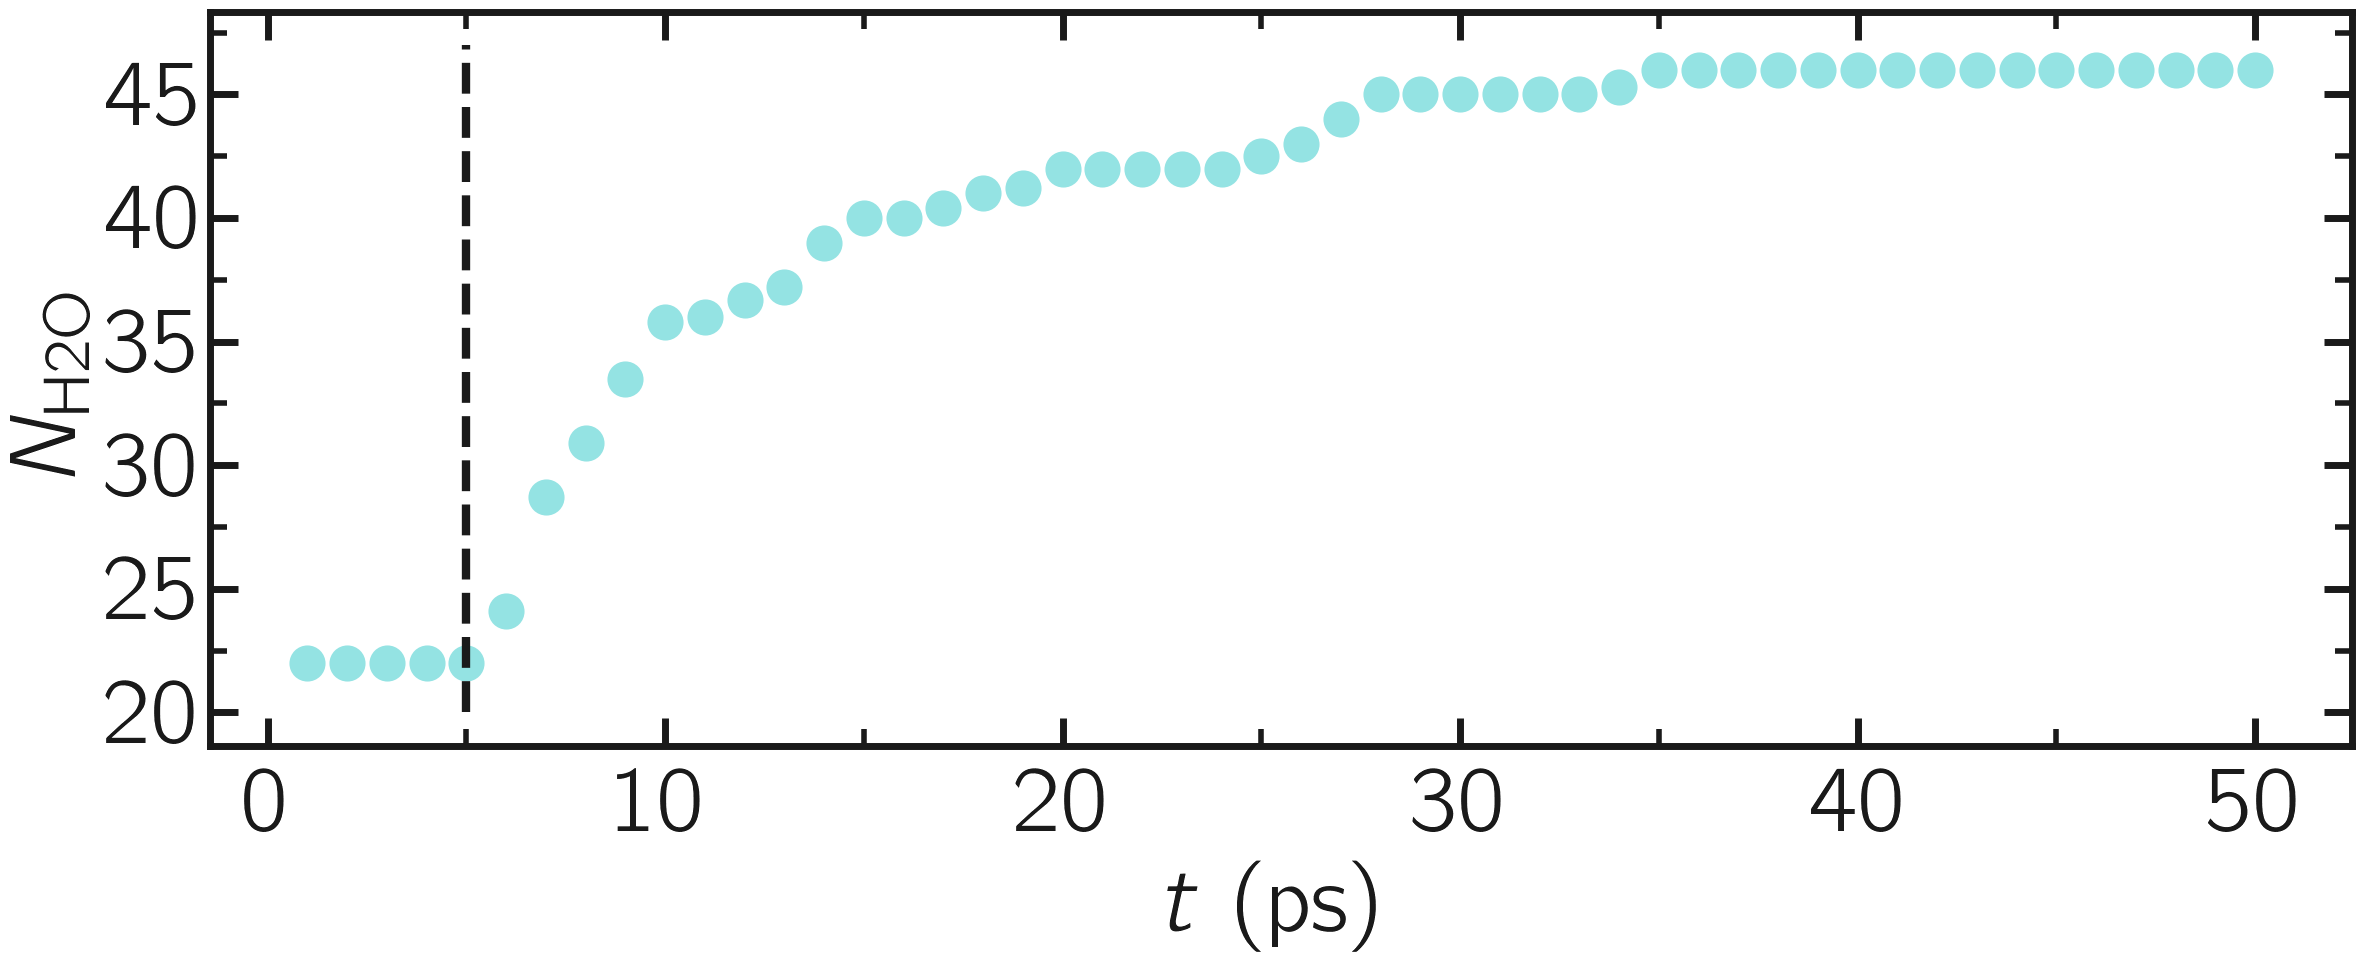
\includegraphics[width=\linewidth]{GCMC-number}
\caption{Number of water molecules $N_\text{H2O}$ as a function of the time $t$.
The dashed vertical line marks the beginning of the GCMC step.}
\label{fig:GCMC-number}
\end{figure}

When you run the simulation, the log file indicates that 840 atoms (i.e. 280 molecules)
were added by the \textit{create\_atoms} command (the exact number you get may differ):
{\normalsize \begin{verbatim}
Created 840 atoms
\end{verbatim}}
You can also see that 258 molecules were immediately deleted, leaving 24 water
molecules (again, the exact number you get may differ):
{\normalsize \begin{verbatim}
Deleted 774 atoms, new total = 642
Deleted 516 bonds, new total = 44
Deleted 258 angles, new total = 22
\end{verbatim}}
After just a few GCMC steps, the number of molecules starts increasing. Once the
crack is filled with water molecules, the number of molecules reaches a plateau
(Figs.\,\ref{fig:GCMC-number}-\ref{fig:GCMC-solvated}). The final number of
molecules depends on the imposed pressure, temperature, and the interaction
between water and silica (i.e. its hydrophilicity). Note that GCMC simulations
of such dense phases are usually slow to converge due to the very low probability
of successfully inserting a molecule. Here, the short simulation duration was
made possible by the use of a large pressure.

\begin{figure}
\centering
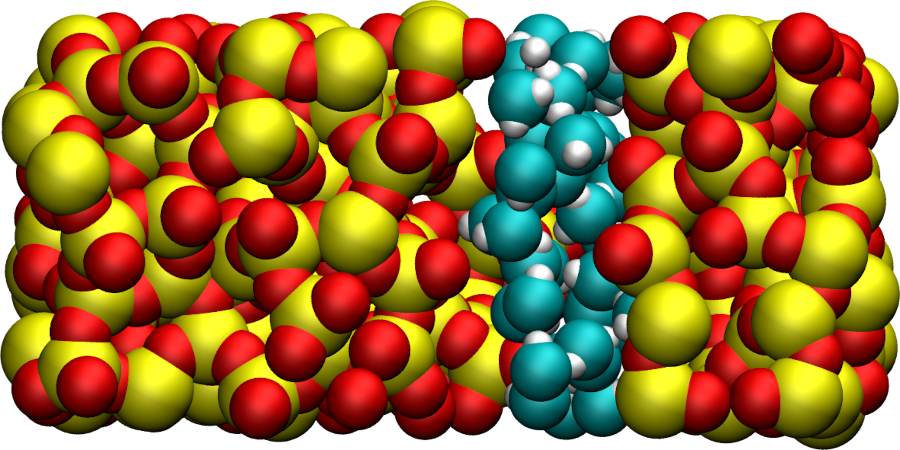
\includegraphics[width=\linewidth]{GCMC-solvated}
\caption{Snapshot of the silica system after the adsorption of water molecules.
The oxygen atoms of the water molecules are represented in cyan, the silicon
atoms in yellow, and the oxygen atoms of the solid in red.}
\label{fig:GCMC-solvated}
\end{figure}

\subsection{Tutorial 7: Free energy calculation}
\label{umbrella-sampling-label}

\begin{figure}
\centering
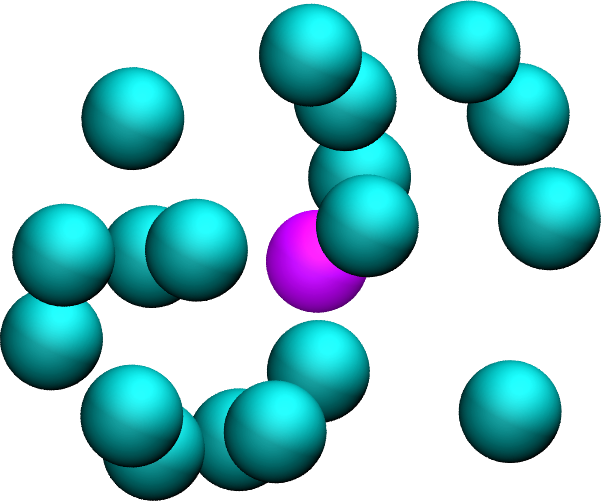
\includegraphics[width=0.55\linewidth]{US}
\caption{Atoms as simulated during \hyperref[umbrella-sampling-label]{Tutorial 7}.
Only the atom colored in pink feels the additional force used for the umbrella
sampling method.}
\label{fig:US}
\end{figure}

\noindent The objective of this tutorial is to measure the free energy profile
of particles across a barrier potential using two methods: free sampling and
umbrella sampling \cite{kastner2011umbrella, allen2017computer, frenkel2023understanding} (Fig.\,\ref{fig:US}).
For simplicity and to reduce computation time, the barrier potential will be
imposed on the atoms with an additional force, mimicking the presence of a repulsive
area in the middle of the simulation box without the need to simulate extra atoms.
The procedure is valid for more complex systems and can be adapted to many other
situations, such as measuring the adsorption barrier near an interface, or for
calculating a translocation barrier through a membrane
\cite{wilson1997adsorption, makarov2009computer, gravelle2021adsorption}.

\subsubsection{Method 1: Free sampling}
The most direct way to calculate a free energy profile is to extract the partition
function from a classical (i.e. unbiased) molecular dynamics simulation, and
then estimate the Gibbs free energy using
\begin{equation}
\Delta G = -RT \ln(p/p_0),
\label{eq:G}
\end{equation}
where $\Delta G$ is the free energy difference, $R$ is the gas constant, $T$
is the temperature, $p$ is the pressure, and $p_0$ is a reference pressure.
As an illustration, let us apply this method to an extremely simple configuration
that consists of a few particles diffusing in a box in the presence of a
position-dependent repelling force that makes the center of the box a relatively
unfavorable area to explore.

\paragraph{Basic LAMMPS parameters}
\noindent Create a folder called \textit{FreeSampling/}, and create an input
script called \textit{input.lmp} in it. Copy the following lines into it:
{\normalsize \begin{verbatim}
variable sigma equal 3.405
variable epsilon equal 0.238
variable U0 equal 1.5*${epsilon}
variable dlt equal 0.5
variable x0 equal 5.0

units real
atom_style atomic
pair_style lj/cut 3.822
pair_modify shift yes
boundary p p p
\end{verbatim}}
Here, we start by defining variables for the Lennard-Jones interaction
$\sigma$ and $\epsilon$ and for the repulsive potential $U$: $U_0$, $\delta$, and $x_0$,
see the analytical expression below. The value of 3.822 for the cut-off was chosen to
create a WCA, purely repulsive, potential \cite{weeks1971role}. It was calculated
as $2^{1/6} \times 3.405$ where $3.405 = \sigma$. The potential is shifted to be
equal to 0 at the cut-off using the \textit{pair\_modify}. The system of unit
\textit{real}, for which energy is in kcal/mol, distance in Ångstrom, or time in
femtosecond, has been chosen for practical reasons: the WHAM algorithm used in
the second part of the tutorial automatically assumes the energy to be in kcal/mol.

\paragraph{System creation and settings}
\noindent Let us define the simulation box and randomly add atoms by copying the
following lines into \textit{input.lmp}:
{\normalsize \begin{verbatim}
region myreg block -25 25 -5 5 -25 25
create_box 1 myreg
create_atoms 1 random 60 341341 myreg &
    overlap 1.5 maxtry 50

mass * 39.95
pair_coeff * * ${epsilon} ${sigma}
neigh_modify every 1 delay 4 check yes
\end{verbatim}}

The variables $U_0$, $\delta$, and $x_0$ defined in the previous subsection are
used here to create the repulsive potential, restricting the atoms from exploring
the center of the box:
\begin{equation}
U = U_0 \left[ \arctan \left( \dfrac{x+x_0}{\delta} \right)
- \arctan \left(\dfrac{x-x_0}{\delta} \right) \right].
\label{eq:U}
\end{equation}
From the derivative of the potential with respect to $x$, we obtain the expression
for the force that will be imposed on the atoms:
\begin{equation}
F= \dfrac{U_0}{\delta} \left[ \dfrac{1}{(x-x_0)^2/\delta^2+1}
- \dfrac{1}{(x+x_0)^2/\delta^2+1} \right].
\label{eq:F}
\end{equation}
Fig.\,\ref{fig:potential} shows the potential $U$ and force $F$ along the $x$ axis.
With $U_0 = 1.5 \epsilon = 0.36\,\text{kcal/mol}$, $U_0$ is of the same order as the
thermal energy $k_\text{B} T = 0.24\,\text{kcal/mol}$, where $k_\text{B} = 0.002\,\text{kcal/mol/K}$
is the Boltzmann constant and $T = 119.8\,\text{K}$ (see below). In this case,
particles are expected to regularly overcome the energy barrier thanks to
the thermal agitation.

\begin{figure}
\centering
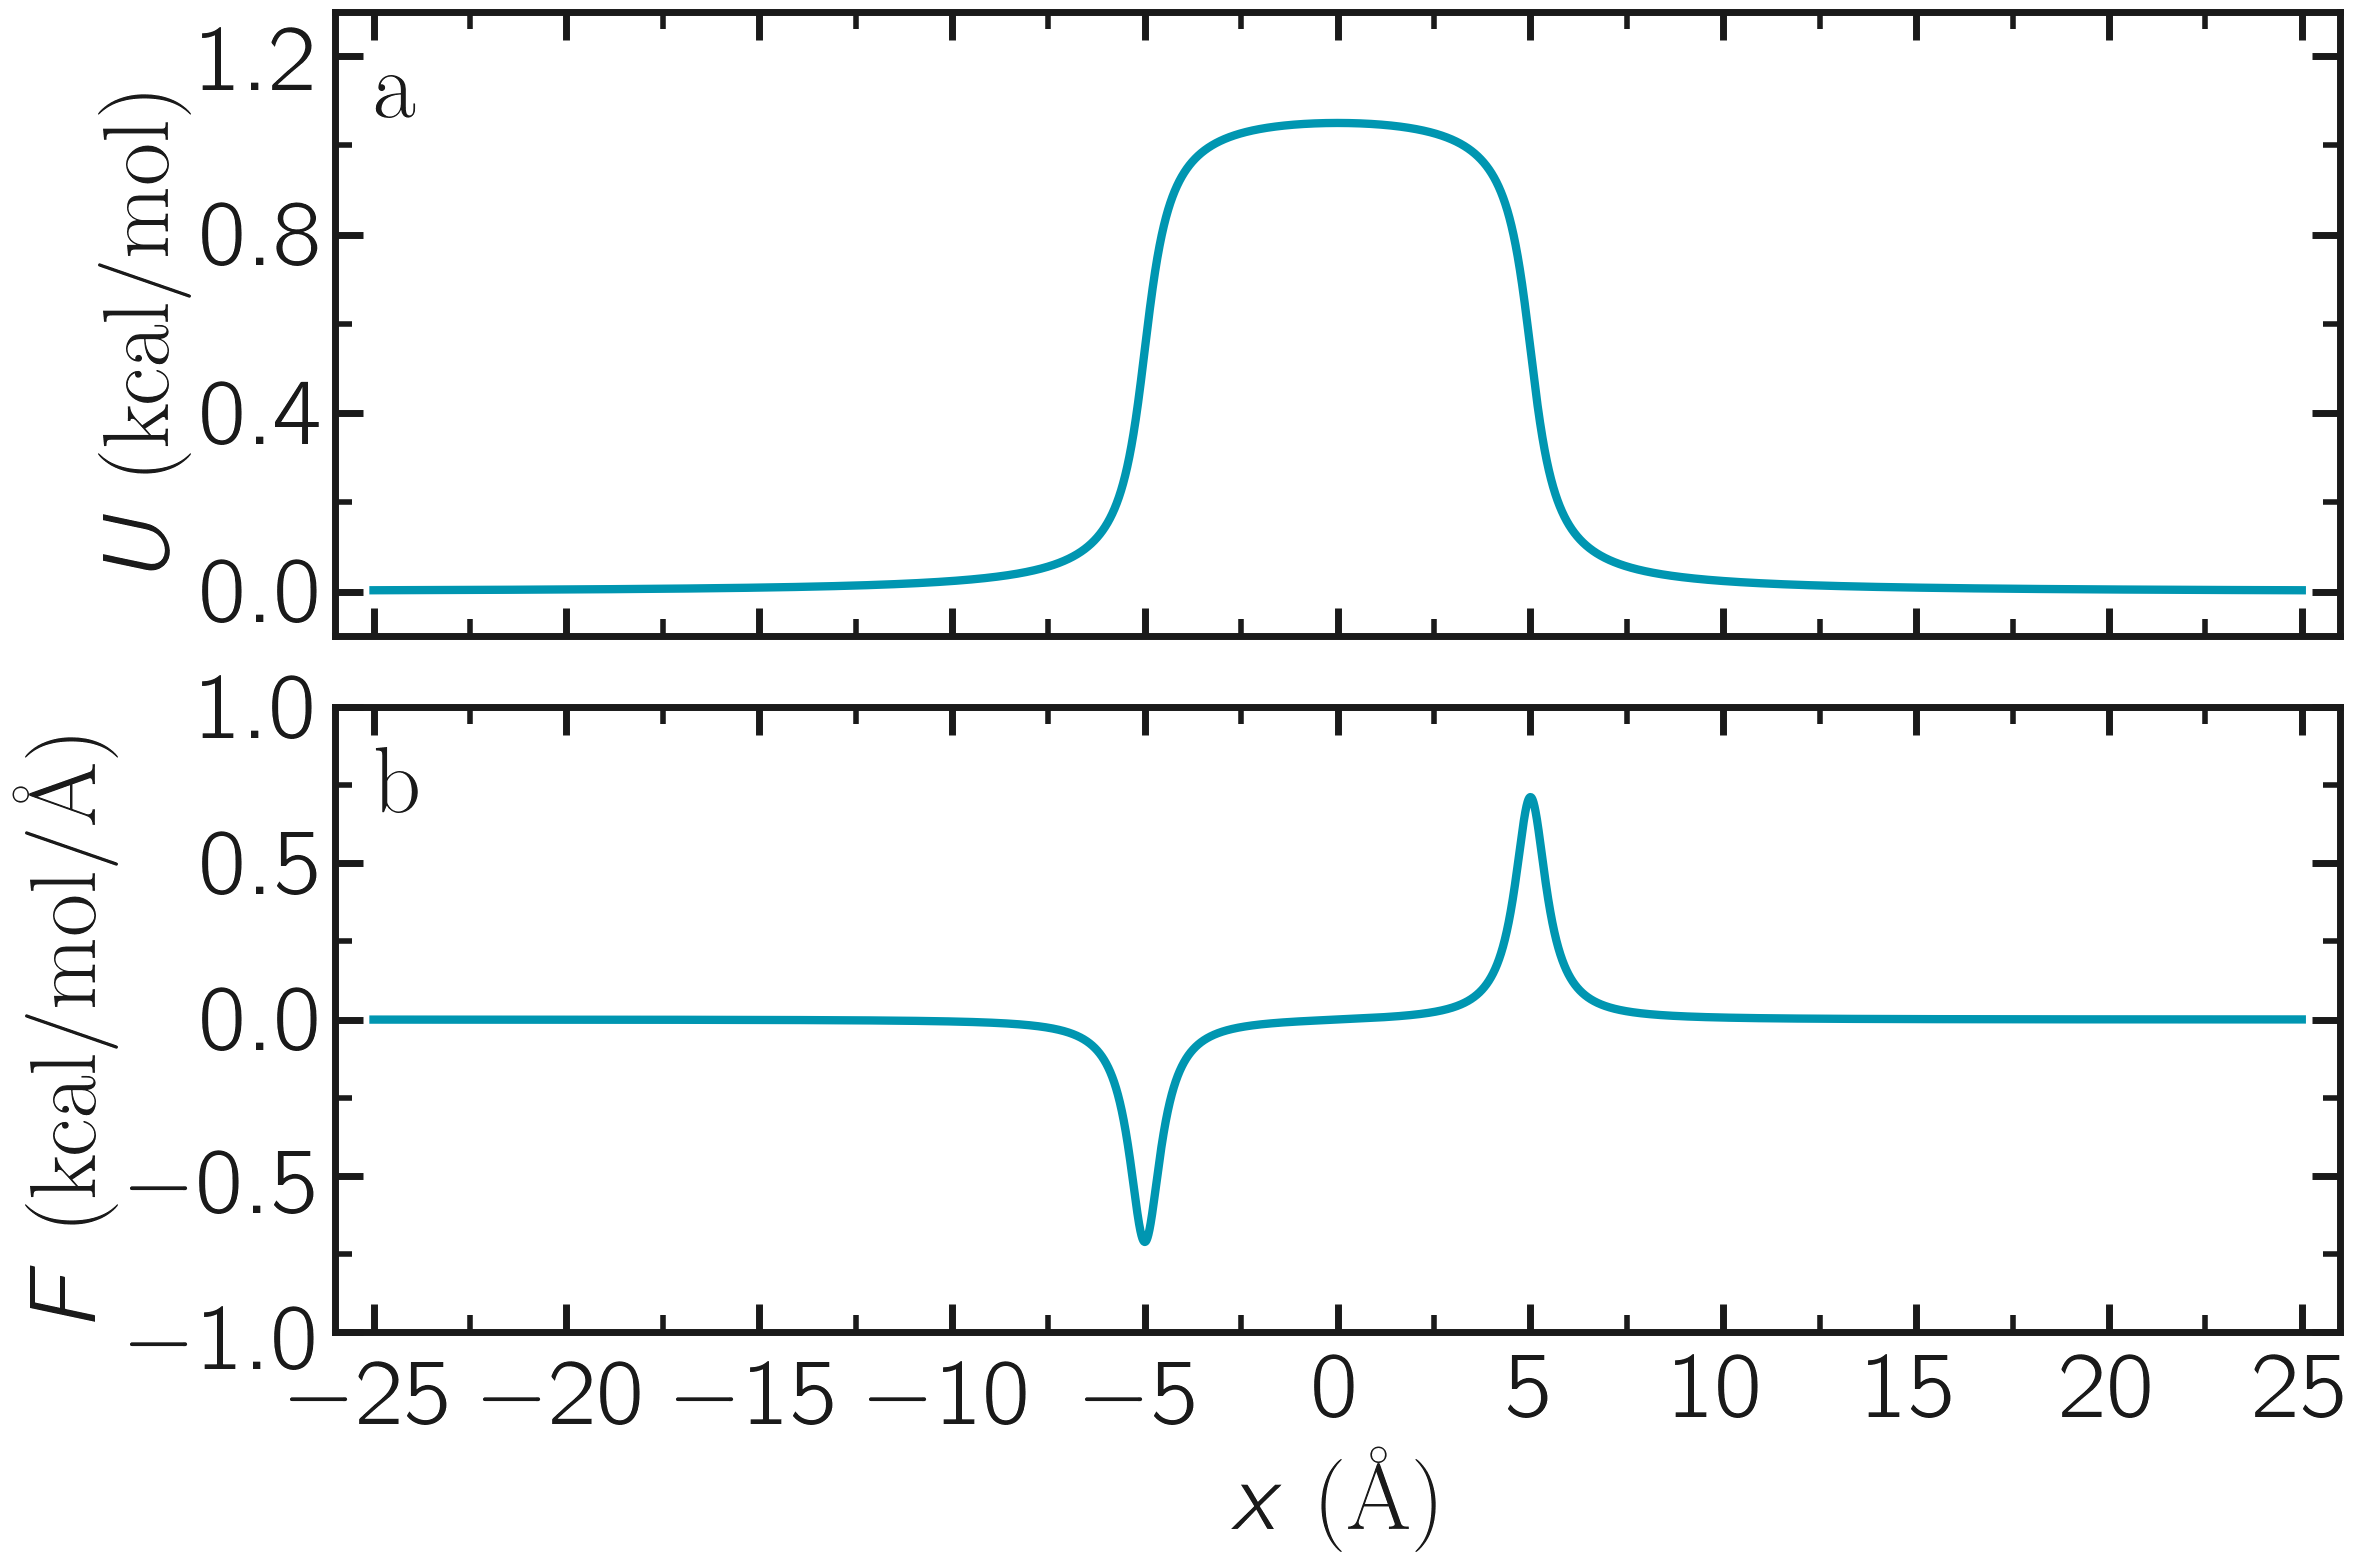
\includegraphics[width=\linewidth]{US-potential}
\caption{Potential $U$ given in Eq.\,\eqref{eq:U} (a) and force $F$ given in
Eq.\,\eqref{eq:F} (b) as a function of the coordinate $x$. Here,
$U_0 = 0.36~\text{kcal/mol}$, $\delta = 0.5~\mathrm{\AA{}}$, and $x_0 = 5~\mathrm{\AA{}}$.}
\label{fig:potential}
\end{figure}

Let us apply energy minimization to the system, and then impose the force $F(x)$
to all of the atoms in the simulation using the \textit{addforce} command. Add
the following lines to \textit{input.lmp}:
{\normalsize \begin{verbatim}
minimize 1e-4 1e-6 100 1000
reset_timestep 0

variable U atom ${U0}*atan((x+${x0})/${dlt})&
    -${U0}*atan((x-${x0})/${dlt})
variable F atom &
    ${U0}/((x-${x0})^2/${dlt}^2+1)/${dlt}&
    -${U0}/((x+${x0})^2/${dlt}^2+1)/${dlt}
fix myadf all addforce v_F 0.0 0.0 energy v_U
\end{verbatim}}
Finally, let us combine the \textit{fix nve} with a \textit{Langevin} thermostat
and run a molecular dynamics simulation:
{\normalsize \begin{verbatim}
fix mynve all nve
fix mylgv all langevin 119.8 119.8 50 1530917
\end{verbatim}}
With these two commands, the MD simulation
is effectively in the NVT ensemble: constant number of atoms $N$, constant volume
$V$, and constant temperature $T$.

To make sure that $1\,\text{ns}$ is long enough, we will record the evolution of
the number of atoms in the central (energetically unfavorable) region called \textit{mymes}
using the \textit{n\_center} variable:
{\normalsize \begin{verbatim}
region mymes block -${x0} ${x0} INF INF INF INF
variable n_center equal count(all,mymes)
thermo_style custom step temp etotal v_n_center
thermo 10000

dump mydmp all image 5000 dump.*.jpg type type &
    shiny 0.1 box yes 0.02 view 0 90 zoom 1.9
dump_modify mydmp backcolor white &
    acolor 1 cyan adiam 1 1 boxcolor black
\end{verbatim}}
A \textit{dump image} was also added for system visualization.

Finally, let us perform an equilibration of 500000 steps
in total, using a timestep of $2\,\text{fs}$ (i.e. a total duration of $1\,\text{ns}$):
{\normalsize \begin{verbatim}
timestep 2.0
run 500000
\end{verbatim}}
Run the simulation with LAMMPS. To ensure that the equilibration of $1\,\text{ns}$ is long
enough, let us have a look at the evolution of the number of atoms in the central region,
$n_\mathrm{center}$. We can see that $n_\mathrm{center}$ reaches
its equilibrium value (which is close to 0) after about $0.1\,\text{ns}$
(Fig.\,\ref{fig:US-density-evolution}). See also a snapshot of the equilibrated
system in Fig.\,\ref{fig:US-system-unbiased}.

\paragraph{Run and data acquisition}
Once the system is equilibrated, let us record the density profile of
the atoms along the $x$ axis using
the \textit{ave/chunk} command. A total of 10 density profiles will be printed.
Add the following line to \textit{input.lmp}:
{\normalsize \begin{verbatim}
unfix myat
undump mydmp
reset_timestep 0

compute cc1 all chunk/atom bin/1d x 0.0 1.0
fix myac all ave/chunk 10 400000 4000000 &
    cc1 density/number file density_profile.dat
dump mydmp all atom 200000 dump.lammpstrj

thermo 100000
run 4000000
\end{verbatim}}
The step count is reset to 0 using \textit{reset\_timestep} to synchronize
with the output times of \textit{fix density/number}. Feel free to increase the
duration of the last run for a better resolved density profile.

\begin{figure}
\centering
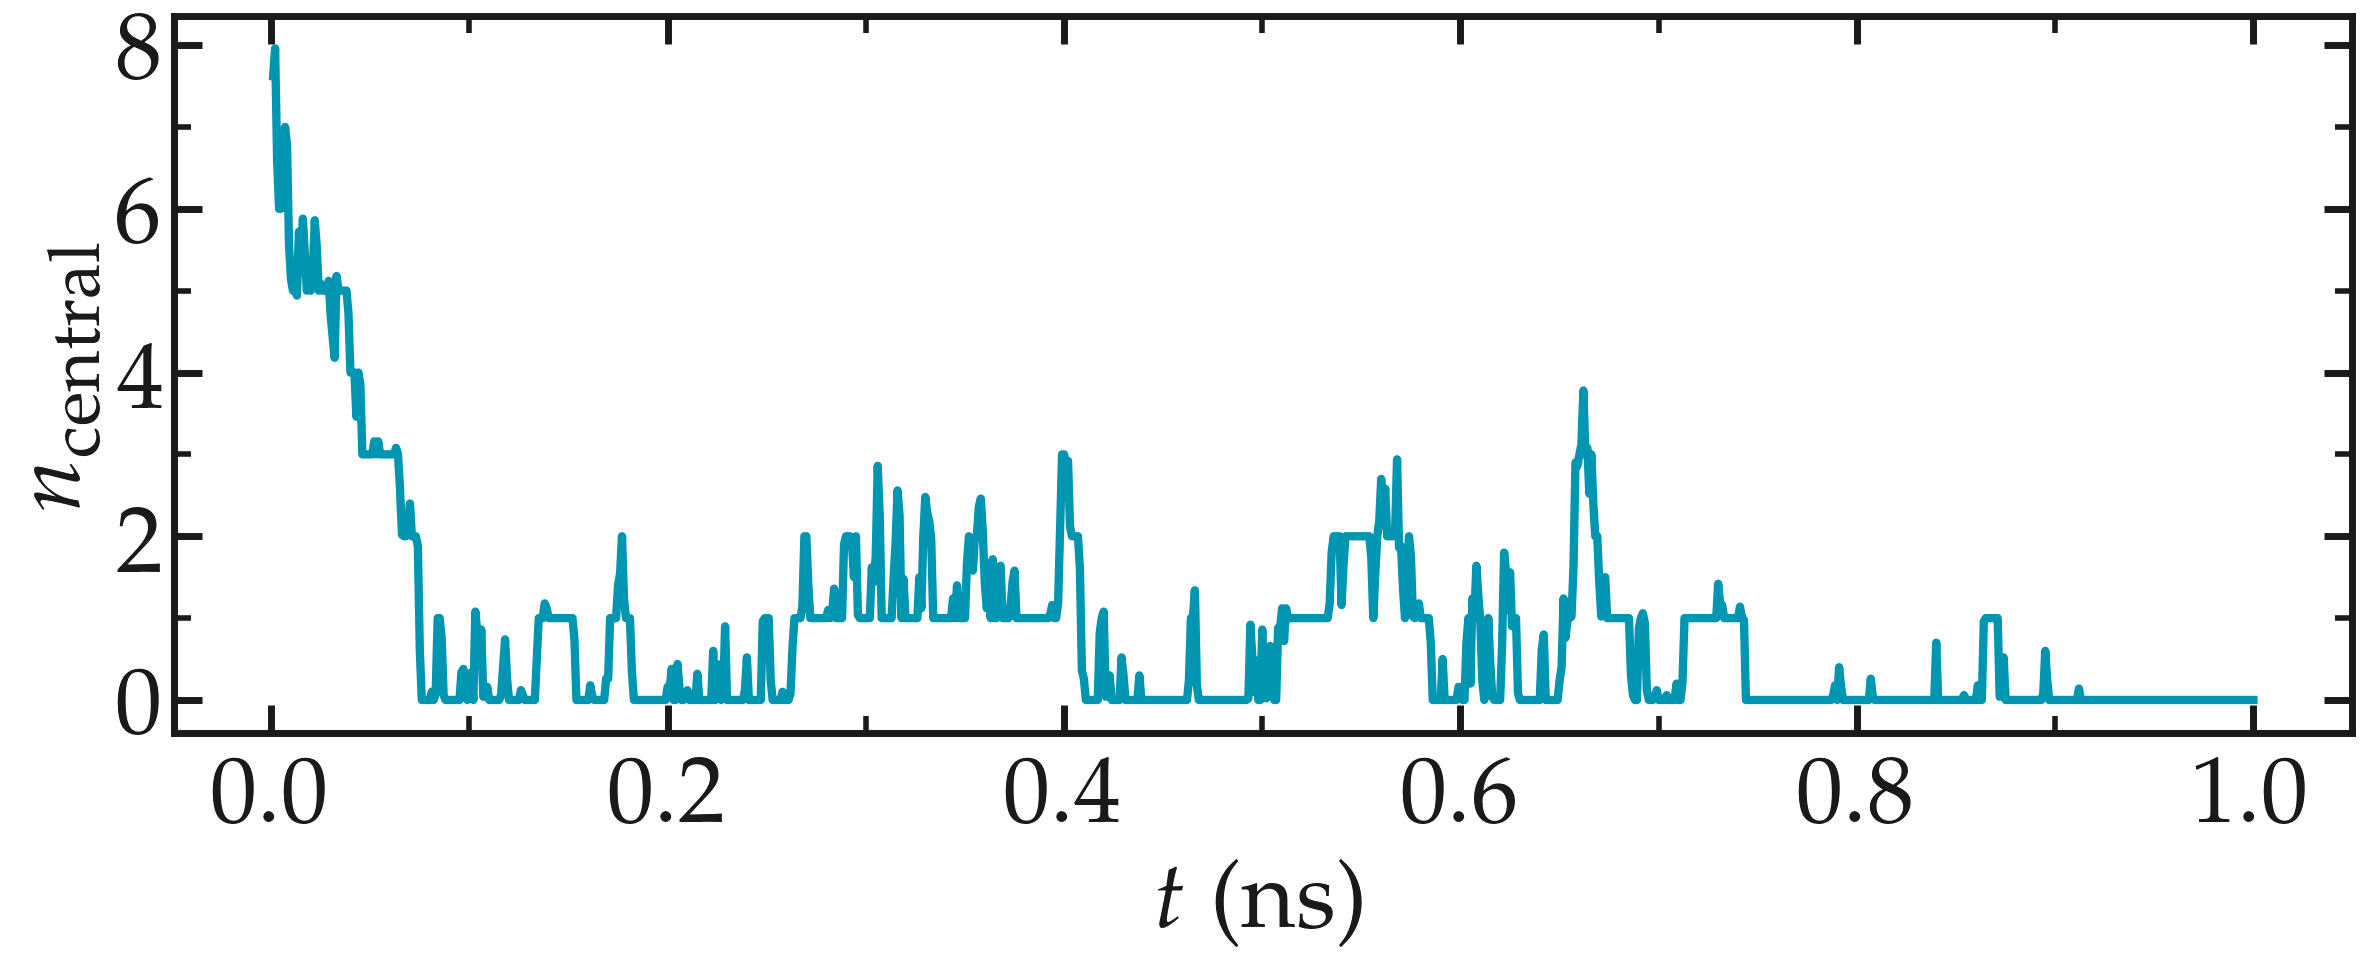
\includegraphics[width=\linewidth]{US-density-evolution}
\caption{Evolution of the number of atoms $n_\text{center}$ in the central
region \textit{mymes} as a function of time $t$ during equilibration. The dark line
serves as a guide for the eyes. Here, $U_0 = 0.36~\text{kcal/mol}$,
$\delta = 0.5~\mathrm{\AA{}}$, and $x_0 = 5~\mathrm{\AA{}}$.}
\label{fig:US-density-evolution}
\end{figure}

\paragraph{Data analysis}

Once the simulation is over, the density profile shows that the density in the center of the box is
about two orders of magnitude lower than inside the reservoir (Fig.\,\ref{fig:US-density}).
Then, let us plot $-R T \ln(\rho/\rho_\mathrm{bulk})$ (i.e. Eq.\,\eqref{eq:G} where
the pressure ratio $p/p_\mathrm{bulk}$ is replaced by the density ratio
$\rho/\rho_\mathrm{bulk}$ assuming the system is an ideal gas) and compare it
with the imposed potential $U$ from Eq.\,\eqref{eq:U} (Fig.\,\ref{fig:US-FreeSampling}).
The value for the reference density $\rho_\text{bulk} = 0.0033~\text{\AA{}}^{-3}$
was estimated by measuring the density of the reservoir from the raw density
profiles. The agreement between the MD results and the imposed energy profile
is reasonable, despite some noise in the central part (where fewer data points
are available due to the repulsive potential).

\begin{figure}
\centering
\includegraphics[width=\linewidth]{US-system-unbiased}
\caption{Snapshot of the system. The density of atoms is lowest in the central
part of the box, \textit{mymes}, due to the additional force $F$. Here,
$U_0 = 0.36~\text{kcal/mol}$, $\delta = 0.5~\mathrm{\AA{}}$, and $x_0 = 5~\mathrm{\AA{}}$.}
\label{fig:US-system-unbiased}
\end{figure}

\begin{figure}
\centering
\includegraphics[width=\linewidth]{US-density}
\caption{Fluid density $\rho$ along the $x$ direction. Here,
$U_0 = 0.36~\text{kcal/mol}$, $\delta = 0.5~\mathrm{\AA{}}$, $x_0 = 5~\mathrm{\AA{}}$,
and reference density $\rho_\text{bulk} = 0.0033~\text{\AA{}}^{-3}$.}
\label{fig:US-density}
\end{figure}

\begin{figure}
\centering
\includegraphics[width=\linewidth]{US-FreeSampling}
\caption{Potential $U$ as a function of $x$ measured using free sampling (blue disks)
compared to the imposed potential given in Eq.\,\eqref{eq:U} (dark line). Here,
$U_0 = 0.36~\text{kcal/mol}$, $\delta = 0.5~\mathrm{\AA{}}$, and $x_0 = 5~\mathrm{\AA{}}$.}
\label{fig:US-FreeSampling}
\end{figure}

\paragraph{The limits of free sampling}
If we increase the value of $U_0$, the average number of atoms in the central
region will decrease, making it difficult to obtain a good resolution for the free
energy profile. For instance, when we run the same simulation using $U_0 = 10 \epsilon$,
which corresponds to a situation where $U_0 \approx 10 k_\text{B} T$, not a single
atom explores the central part of the simulation box during the 8 ns of simulation.
In this case, using an enhanced sampling method is preferred; see the next section.

\subsubsection{Method 2: Umbrella sampling}
Umbrella sampling is a biased molecular dynamics method in which additional forces
are added to a chosen atom to force it to explore the more unfavorable areas of
the system \cite{kastner2011umbrella, allen2017computer, frenkel2023understanding}.
Here, to encourage one of the atoms to explore the central region of the box,
we apply a potential $V$ and force it to move along the $x$-axis. The chosen path
is called the axis of reaction. Several simulations (called windows) will be
conducted with varying positions for the center of the applied biasing. The results
will be analyzed using the weighted histogram analysis method (WHAM) \cite{kumar1992weighted},
which allows for the removal of the biasing effect and ultimately deduces the
unbiased free energy profile.

\paragraph{LAMMPS input script}
Create a new folder called \textit{BiasedSampling/}, and create a new input file
called \textit{input.lmp} in it, and copy the following lines:
{\normalsize \begin{verbatim}
variable sigma equal 3.405
variable epsilon equal 0.238
variable U0 equal 10*${epsilon}
variable dlt equal 0.5
variable x0 equal 5.0
variable k equal 1.5

units real
atom_style atomic
pair_style lj/cut 3.822
pair_modify shift yes
boundary p p p

region myreg block -25 25 -5 5 -25 25
create_box 2 myreg
create_atoms 2 single 0 0 0
create_atoms 1 random 5 341341 myreg &
    overlap 1.5 maxtry 50

mass * 39.948
pair_coeff * * ${epsilon} ${sigma}
neigh_modify every 1 delay 4 check yes
group topull type 2

minimize 1e-4 1e-6 100 1000
reset_timestep 0

variable U atom ${U0}*atan((x+${x0})/${dlt})&
    -${U0}*atan((x-${x0})/${dlt})
variable F atom &
    ${U0}/((x-${x0})^2/${dlt}^2+1)/${dlt}&
    -${U0}/((x+${x0})^2/${dlt}^2+1)/${dlt}
fix pot all addforce v_F 0.0 0.0 energy v_U

fix mynve all nve
fix mylgv all langevin 119.8 119.8 50 1530917
timestep 2.0
thermo 100000
run 500000
reset_timestep 0

dump mydmp all image 1000000 dump.*.jpg type &
type shiny 0.1 box yes 0.02 view 0 90 zoom 1.9
dump_modify mydmp backcolor white &
    acolor 1 cyan adiam 1 1 &
    acolor 2 pink adiam 1 1 &
    boxcolor black
\end{verbatim}}
So far, this code resembles that of Method 1, except for the additional particle
of type 2. Particles of type 1 and 2
are identical, having the same mass and Lennard-Jones parameters. However, the
particle of type 2 will additionally be exposed to the biasing potential
$V$ (Fig.\,){fig:US-system-biased}).

Let us create a loop with 50 steps, and move progressively the center of the
bias potential by an increment of 0.1 nm. Add the following lines to \textit{input.lmp}:
{\normalsize \begin{verbatim}
variable a loop 50
label loop
variable xdes equal ${a}-25
variable xave equal xcm(topull,x)
fix mytth topull spring tether ${k} &
    ${xdes} 0 0 0
run 200000
fix myat1 all ave/time 10 10 100 v_xave &
    v_xdes file data/position.${a}.dat
run 1000000
unfix myat1
next a
jump SELF loop
\end{verbatim}}
A folder called \textit{data/} needs to be created within \textit{BiasedSampling/}.
The spring command serves to impose the additional harmonic potential $V$ with
the spring constant $k$. Note that the value of $k$ should be chosen with care,
if $k$ is too small, the particle won't follow the biasing potential center,
and if $k$ is too large, there will be no overlapping between the different windows.
The center of the harmonic potential $x_\text{des}$ successively takes values
from -25 to 25. For each value of $x_\text{des}$, an equilibration step of 0.4 ns
is performed, followed by a step of 2 ns during which the position along $x$ of
the particle is saved in data files (one data file per value of $x_\text{des}$).
You can always increase the duration of the runs for better samplings. Run the
\textit{input.lmp}  file using LAMMPS.

\begin{figure}
\centering
\includegraphics[width=\linewidth]{US-system-biased}
\caption{Snapshot of the system with atoms of type 1 in cyan and the single atom
of type 2 in pink. Only the atom of type 2 explores the central part of the box,
\textit{mymes}, due to its additional biasing potential $V$. Here,
$U_0 = 2.38~\text{kcal/mol}$, $\delta = 0.5~\mathrm{\AA{}}$, and $x_0 = 5~\mathrm{\AA{}}$.}
\label{fig:US-system-biased}
\end{figure}

\paragraph{WHAM algorithm}
\noindent To generate the free energy profile from the density distribution,
let us use the WHAM algorithm as implemented by Marc Grossfield \cite{grossfieldimplementation}.
You can download it from \href{http://membrane.urmc.rochester.edu/?page_id=126}{Alan Grossfield}
website, and compile it by typing in the terminal:
{\normalsize
\begin{verbatim}
cd wham
make clean
make
\end{verbatim}
}
\noindent The compilation creates an executable called \textit{wham} that you can
copy in the \textit{BiasedSampling/} folder. To apply the WHAM algorithm to our
simulation, we first need to create a metadata file. This file simply contains
\begin{itemize}
\item the paths to all the data files,
\item the value of $x_\text{des}$,
\item and the values of $k$.
\end{itemize}
Download the \href{https://raw.githubusercontent.com/lammpstutorials/lammpstutorials-article/main/files/tutorial7/metadata.dat}{\textit{metadata.dat}}
file I have written and save it in \textit{BiasedSampling/}. Then, simply run the
following command in the terminal:
{\normalsize
\begin{verbatim}
./wham -25 25 50 1e-8 119.8 0 \
    metadata.dat PMF.dat
\end{verbatim}
}
where -25 and 25 are the boundaries, 50 is the number of bins, 1e-8 is the tolerance,
and 119.8 is the temperature. A file called \textit{PMF.dat} has been created,
containing the free energy profile in kcal/mol. Again, one can compare the result of
the PMF with the imposed potential $U$, demonstrating excellent agreement
(Fig.\,\ref{fig:US-freenergy}). We can see that the agreement is quite good despite
the very short calculation time and the very high value for the energy barrier.
Obtaining the same results with Free Sampling would require performing extremely
long and costly simulations.

\begin{figure}
\centering
\includegraphics[width=\linewidth]{US-freenergy}
\caption{Potential $U$ as a function of $x$ measured using umbrella sampling
(blue disks) compared to the imposed potential given in Eq.\,\eqref{eq:U}
(dark line). Here, $U_0 = 2.38~\text{kcal/mol}$, $\delta = 0.5~\mathrm{\AA{}}$,
and $x_0 = 5~\mathrm{\AA{}}$.}
\label{fig:US-freenergy}
\end{figure}

\section*{Author Contributions}
% S.G. to update
S.G. conceived and wrote all the online tutorials and underlying Sphinx documentation
for \href{https://lammpstutorials.github.io}{lammpstutorials.github.io}.

\noindent A.K. wrote the LAMMPS GUI software and helped revise the
tutorials for use with it.

\noindent J.G. is the principal author of fix bond/react and type label
support in LAMMPS.  He revised tutorials to use type labels.
% and contributed the eighth tutorial using fix bond/react (?).

\section*{Potentially Conflicting Interests}

There are no conflicting interests to declare.

\section*{Funding Information}

S.G. acknowledges funding from the European Union's Horizon 2020 research and
innovation programme under the Marie Skłodowska-Curie grant agreement N$^\circ\;101065060$.

\noindent A.K. acknowledges financial support by Sandia National Laboratories under
POs 2149742 and 2407526.

\section*{Author Information}
\makeorcid

\bibliography{journal-article}

%%%%%%%%%%%%%%%%%%%%%%%%%%%%%%%%%%%%%%%%%%%%%%%%%%%%%%%%%%%%
%%% APPENDICES
%%%%%%%%%%%%%%%%%%%%%%%%%%%%%%%%%%%%%%%%%%%%%%%%%%%%%%%%%%%%

\begin{appendices}
  \section{Using LAMMPS-GUI}
  \label{using-lammps-gui}

  { \normalsize
\begin{verbatim}
  lammps-gui input.lmp
\end{verbatim}
  }

  \section{Compiling LAMMPS from Source on Linux}
  \label{compiling-lammps-label}
  FIXME: add section

  % AK: For beginner we recommend CMake and a current Linux OS (at least Ubuntu 22.04LTS, RHEL 9 (and Alma, or Rocky), Fedora 39)
  % The Linux system must support packages for software development installed and the corresponding development packages for compiling with MPI

  % AK: a mostly complete list of packages for different Linux flavors can be inferred from singularity/apptainer container definition files in "tools/singularity"

%Depending on your operating system (i.e. Linux, macOS, or Windows), the procedure may differ. LAMMPS must be compiled with the following packages:
%\begin{itemize}
%\item MANYBODY
%\item MOLECULE
%\item KSPACE
%\item RIGID
%\item REAXFF
%\item EXTRA-DUMP
%\end{itemize}

% AK: for non-Linux OS please refer to LAMMPS Manual.


  \section{Running LAMMPS in Parallel with MPI}
  \label{parallel-lammps-label}
  FIXME: add section
\end{appendices}

\end{document}

%%% Local Variables:
%%% mode: latex
%%% TeX-master: t
%%% End:
